	%% ----------------------------------------------------------------
%% Thesis.tex -- MAIN FILE (the one that you compile with LaTeX)
%% ---------------------------------------------------------------- 

% Set up the document
\documentclass[letterpaper, 11pt, oneside]{Thesis}  % Use the "Thesis" style, based on the ECS Thesis style by Steve Gunn
\graphicspath{Figures/}  % Location of the graphics files (set up for graphics to be in PDF format)
%AQUI INSERTE COSAS RARAS
\usepackage{amsmath}

\usepackage[final]{feynmp} 
 \DeclareGraphicsRule{*}{mps}{*}{} 
 \makeatletter 
 \def\endfmffile{% 
 	\fmfcmd{\p@rcent\space the end.^^J% 
 			end.^^J% 
 			endinput;}% 
 	\if@fmfio 
 		\immediate\closeout\@outfmf 
 	\fi 
 	\ifnum\pdfshellescape=\@ne 
 		\immediate\write18{mpost \thefmffile}% 
 	\fi} 
 \makeatother 
%AQUI INSERTE COSAS RARAS




% Include any extra LaTeX packages required
\usepackage[square, numbers, comma, sort&compress]{natbib}  % Use the "Natbib" style for the references in the Bibliography
\usepackage[spanish, es-tabla]{babel}
\usepackage[rightcaption]{sidecap}
\usepackage{verbatim}  % Needed for the "comment" environment to make LaTeX comments
\usepackage{vector}  % Allows "\bvec{}" and "\buvec{}" for "blackboard" style bold vectors in maths
\hypersetup{urlcolor=blue, colorlinks=true}  % Colours hyperlinks in blue, but this can be distracting if there are many links.
\def\spanishoperators{}

%% ----------------------------------------------------------------
\begin{document}
%AQUI INSERTE COSAS RARAS
\unitlength=1mm 
%AQUI INSERTE COSAS RARAS



\frontmatter      % Begin Roman style (i, ii, iii, iv...) page numbering

% Set up the Title Page
\title  {Integrales de Trayectoria y Espacios Curvos}
\authors  {\texorpdfstring
            {\href{diegoa_baronm@hotmail.com}{Diego Alberto Barón Moreno}}
            {Author Name}
            }
\addresses  {\groupname\\\deptname\\\univname}  % Do not change this here, instead these must be set in the "Thesis.cls" file, please look through it instead
\date       {\today}
\subject    {}
\keywords   {}

\maketitle
%% ----------------------------------------------------------------

\setstretch{1.3}  % It is better to have smaller font and larger line spacing than the other way round

% Define the page headers using the FancyHdr package and set up for one-sided printing
\fancyhead{}  % Clears all page headers and footers
\rhead{\thepage}  % Sets the right side header to show the page number
\lhead{}  % Clears the left side page header

\pagestyle{fancy}  % Finally, use the "fancy" page style to implement the FancyHdr headers

%% ----------------------------------------------------------------
% Declaration Page required for the Thesis, your institution may give you a different text to place here
%\Declaration{

%\addtocontents{toc}{\vspace{1em}}  % Add a gap in the Contents, for aesthetics

%I, AUTHOR NAME, declare that this thesis titled, `THESIS TITLE' and the work presented in it are my own. I confirm that:

%\begin{itemize} 
%\item[\tiny{$\blacksquare$}] This work was done wholly or mainly while in candidature for a research degree at this University.
 
%\item[\tiny{$\blacksquare$}] Where any part of this thesis has previously been submitted for a degree or any other qualification at this University or any other institution, this has been clearly stated.
 
%\item[\tiny{$\blacksquare$}] Where I have consulted the published work of others, this is always clearly attributed.
 
%\item[\tiny{$\blacksquare$}] Where I have quoted from the work of others, the source is always given. With the exception of such quotations, this thesis is entirely my own work.
 
%\item[\tiny{$\blacksquare$}] I have acknowledged all main sources of help.
 
%\item[\tiny{$\blacksquare$}] Where the thesis is based on work done by myself jointly with %others, I have made clear exactly what was done by others and what I have contributed myself.
%\\
%\end{itemize}
 
 
%Signed:\\
%\rule[1em]{25em}{0.5pt}  % This prints a line for the signature
 
%Date:\\
%\rule[1em]{25em}{0.5pt}  % This prints a line to write the date
%}
%\clearpage  % Declaration ended, now start a new page
%
%% ----------------------------------------------------------------
% The "Funny Quote Page"
\pagestyle{empty}  % No headers or footers for the following pages

\null\vfill
% Now comes the "Funny Quote", written in italics
\textit{``Si ayudo a una sola persona a tener esperanza, no habré vivido en vano.''}

\begin{flushright}
Martin Luther King
\end{flushright}

\vfill\vfill\vfill\vfill\vfill\vfill\null
\clearpage  % Funny Quote page ended, start a new page
%% ----------------------------------------------------------------

% The Abstract Page
\addtotoc{Resumen}  % Add the "Abstract" page entry to the Contents
\abstract{
\addtocontents{toc}{\vspace{1em}}  % Add a gap in the Contents, for aesthetics

En este trabajo pretendo presentar de una manera organizada y concisa el compendio de los temas que he estudiado durante los últimos semestres de mi carrera, en partícular la temática tratada son las intregrales de trayectoria. El primer capítulo trata sobre las integrales de trayectoria en espacio plano (espacio-tiempo de curvatura nula) en este capítulo empiezo con la definción del propagador y la aplicación de este formalismo a problemas de primera cuantización, luego en lo que sigue se estudia el método conocido como álgebra de corrientes (un metodo basado en integrales de trayectoria) para estudiar los problemas de segunda cuantización, esto incluye campos escalares, campos fermiónicos y para finalizar el capítulo se hace una presentación de las teorías Gauge, los campos de Yang-Mills y el método de Faddeev-Popov.
\\
\\
Para el segundo capítulo los esfuerzos se centran en tratar el problema de la cuantización en espacios curvos, en la primera sección se realiza una presentación introductoria de teorías clásicas de campo en espacios curvos para luego estudiar integrales de trayectoria en problemas de primera cuantización en variedades generales. Este estudio incluye la deducción del propagador para la ecuación de Schrödinger generalizada, las transformaciones de coordenadas y la utilidad de este formalismo para resolver problemas de interés en mecánica cuántica, como el átomo de Hidrógeno, utilizando el método de integrales de trayectoria. En la sección final se ha incluído un aporte propio que creemos no está reportado en la literatura y es el cálculo del corrimiento de líneas de interferencia en el efecto Sagnac, calculado vía de integrales de trayectoria. 
}

\clearpage  % Abstract ended, start a new page
%% ----------------------------------------------------------------

\setstretch{1.3}  % Reset the line-spacing to 1.3 for body text (if it has changed)

% The Acknowledgements page, for thanking everyone
\acknowledgements{
\addtocontents{toc}{\vspace{1em}}  % Add a gap in the Contents, for aesthetics

En el tiempo que ha pasado desde que comencé mis estudios he conocido a muchas buenas personas que han ayudado a que este trabajo sea posible, no solo desde un punto de vista académico, sino brindadome pequeños momentos fuera de la academia. Quiero agradecer a mi asesor Nelson Vanegas por su esfuerzo a la hora de guiarme a lo largo de mi carrera, no sólo con su consejo académico sino también con pequeñas sugerencias que han ayudado a convertirme en un mejor profesional, tengo que decir que siento una gran satisfacción de haberme acoplado a su metodología de trabajo, si bien al principio fue difícil entender la libertad que tenía de trabajar a mi ritmo y de no sentir  excesiva presión en alguna dirección, con el tiempo empecé a sentir que esto generaba independencia y criterio. No solo han sido espacios académicos los que hemos compartido y no quiero dejar pasar que también han sido buenos momentos los que hemos pasado fuera de las aulas.
\\
\\
Sin duda alguna, debo agradecer a mis padres por su constante apoyo, en especial a mi madre, Gloria Moreno, con su amor y constante trabajo es responsable de todas las cosas que he hecho en mi vida, incluyendo esta tesis. Siempre ha sido una motivación que ella esté orgullosa de mi. También quiero mencionar a mi hermano Andrés Barón, quién ha sido una excelente compañia durante toda mi vida, finalmente debo nombrar a Rocio Barón y Maria Wandurraga, mi tía y mi abuela, dos mujeres que nunca se cansan de ser buenas conmigo, gracias. Ahora quiero agradecer a todos mis compañeros y amigos, han sido muchos espacios los que hemos compartido: clases, almuerzos, deportes, estudio... sin su apoyo nada de esto hubiera sido posible: Juan Espejo, Juan Luis Restrepo, Luis Santander, Cesar Arroyo, Natalia Osorio, Sergio Vallejo, Luis Ribero, Laura Arboleda, Camilo Santa, Santiago Quintero, Alexis Gonzáles, Delio Jaramillo, Santiago Montoya. 
\\
\\
Quiero mencionar también a Oscar Zapata un profesor excelente e incansable, gracias por todos los consejos y cursos en los que tuve el placer de ser su alumno, agradecer al profesor Diego Restrepo por haberme dado su confianza a la hora de aceptarme en el Grupo de Fenomenología de Interacciones Fundamentales (GFIF) y otros tantos asuntos administrativos. Quiero agradecer también a mis buenos amigos de toda la vida, gracias por todos los momentos de distracción, siempre son necesarios. A mi novia, gracias por creer en mi trabajo y animarme cuando ha hecho falta.
\\
\\
Finalmente agradecer a la Universidad de Antioquia, a todos los profesores y al resto del personal, sin ellos el sueño de ser Físico no hubiese sido posible y tampoco este trabajo, que si bien, en algún momento me tuvo bastante estresado, sin duda disfruté mucho... 
}
\clearpage  % End of the Acknowledgements
%% ----------------------------------------------------------------

\pagestyle{fancy}  %The page style headers have been "empty" all this time, now use the "fancy" headers as defined before to bring them back


%% ----------------------------------------------------------------
\renewcommand{\contentsname}%
    {Tabla de Contenido}%
	
\lhead{\emph{Contents}}  % Set the left side page header to "Contents"
\tableofcontents  % Write out the Table of Contents

%% ----------------------------------------------------------------

\lhead{\emph{Integrales de trayectoria y espacios curvos.}}  % Set the left side page header to "List if Figures"
\listoffigures  % Write out the List of Figures

%% ----------------------------------------------------------------
%\lhead{\emph{List of Tables}}  % Set the left side page header to "List of Tables"
%\listoftables  % Write out the List of Tables

%% ----------------------------------------------------------------
%\setstretch{1.5}  % Set the line spacing to 1.5, this makes the following tables easier to read
%\clearpage  % Start a new page
%\lhead{\emph{Abbreviations}}  % Set the left side page header to "Abbreviations"
%\listofsymbols{ll}  % Include a list of Abbreviations (a table of two columns)
%{
% \textbf{Acronym} & \textbf{W}hat (it) \textbf{S}tands \textbf{F}or \\
%\textbf{LAH} & \textbf{L}ist \textbf{A}bbreviations \textbf{H}ere \\

%}

%% ----------------------------------------------------------------
%\clearpage  % Start a new page
%\lhead{\emph{Physical Constants}}  % Set the left side page header to "Physical Constants"
%\listofconstants{lrcl}  % Include a list of Physical Constants (a four column table)
%{
% Constant Name & Symbol & = & Constant Value (with units) \\
%Speed of Light & $c$ & $=$ & $2.997\ 924\ 58\times10^{8}\ \mbox{ms}^{-\mbox{s}}$ (exact)\%\

%}

%% ----------------------------------------------------------------
%\clearpage  %Start a new page
%\lhead{\emph{Symbols}}  % Set the left side page header to "Symbols"
%\listofnomenclature{lll}  % Include a list of Symbols (a three column table)
%{
% symbol & name & unit \\
%$a$ & distance & m \\
%$P$ & power & W (Js$^{-1}$) \\
%& & \\ % Gap to separate the Roman symbols from the Greek
%$\omega$ & angular frequency & rads$^{-1}$ \\
%}
%% ----------------------------------------------------------------
% End of the pre-able, contents and lists of things
% Begin the Dedication page

\setstretch{1.3}  % Return the line spacing back to 1.3

\pagestyle{empty}  % Page style needs to be empty for this page
\dedicatory{Dedicado a mi madre\ldots Una luchadora.	}

\addtocontents{toc}{\vspace{2em}}  % Add a gap in the Contents, for aesthetics


%% ----------------------------------------------------------------
\mainmatter	  % Begin normal, numeric (1,2,3...) page numbering
\pagestyle{fancy}  % Return the page headers back to the "fancy" style

% Include the chapters of the thesis, as separate files
% Just uncomment the lines as you write the chapters

\chapter{Introducción}
 % Introduction

\chapter{Integrales de trayectoria	 en espacio plano.}
El formalismo más común de la mecánica cuantica se deriva de cambiar las variables clásicas de posición y momentum ($p$ y $q$) por operadores que obedecen el álgebra:
\begin{equation}
[\hat{q},\hat{p}]=i\hbar.
\end{equation}
Esta relación se conoce como la condción de cuantización de Heisenberg, en general en la mecánica cuantica de operadores estos últimos viven en un espacio de Hilbert.
\\
\\
La formulación de integrales de camino se basa en la noción de \textbf{propagador}, esta función es tal que dada una función de onda en un instante de tiempo $t_1$, $\psi(x_1,t_1)$ da la evolucion hasta un instante de tiempo $t_2$, entregando $\psi(x_2,t_2)$. En cierta manera es parecido al principio de Huygens:
\begin{equation}
\psi(x_f,t_f)=\int K(q_f,t_f;q_i,t_i)\psi(q_i,t_i)dq_i.
\end{equation}
De acuerdo con la mecánica cuántica $\psi(q_f,t_f)$ representa la probabilidad de que una partícula se encuentre en un punto $q_f$ en el instante de tiempo $t_f$, por tanto $K(q_f,t_f;q_i,t_i)$ representa la amplitud de probabilidad de transición entre un estado ($q_i,t_i$) y ($q_f,t_f$).
\begin{equation}
P(q_f,t_f;q_i,t_i)=\Vert K(q_f,t_f;q_i,t_i) \Vert^2,
\end{equation}
si dividimos el intervalo de tiempo en $t_i\rightarrow t \rightarrow t_f$, tenemos de la definición de $K$:
\begin{eqnarray}
\nonumber \psi(q_f,t_f)&=&\int\int K(q_f,t_f;q,t)K(q,t;q_i,t_i)dqdq_i\\
\Rightarrow K(q_f,t_f;q_i,t_i)&=&\int dq K(q_f,t_f;q,t)K(q,t;q_i,t_i).
\end{eqnarray}
Como ejemplo de lo anterior podemos analizar el experimento de la doble rendija. En la Figura 1 encontramos un esquema de este:
\begin{figure}[h]
\centering
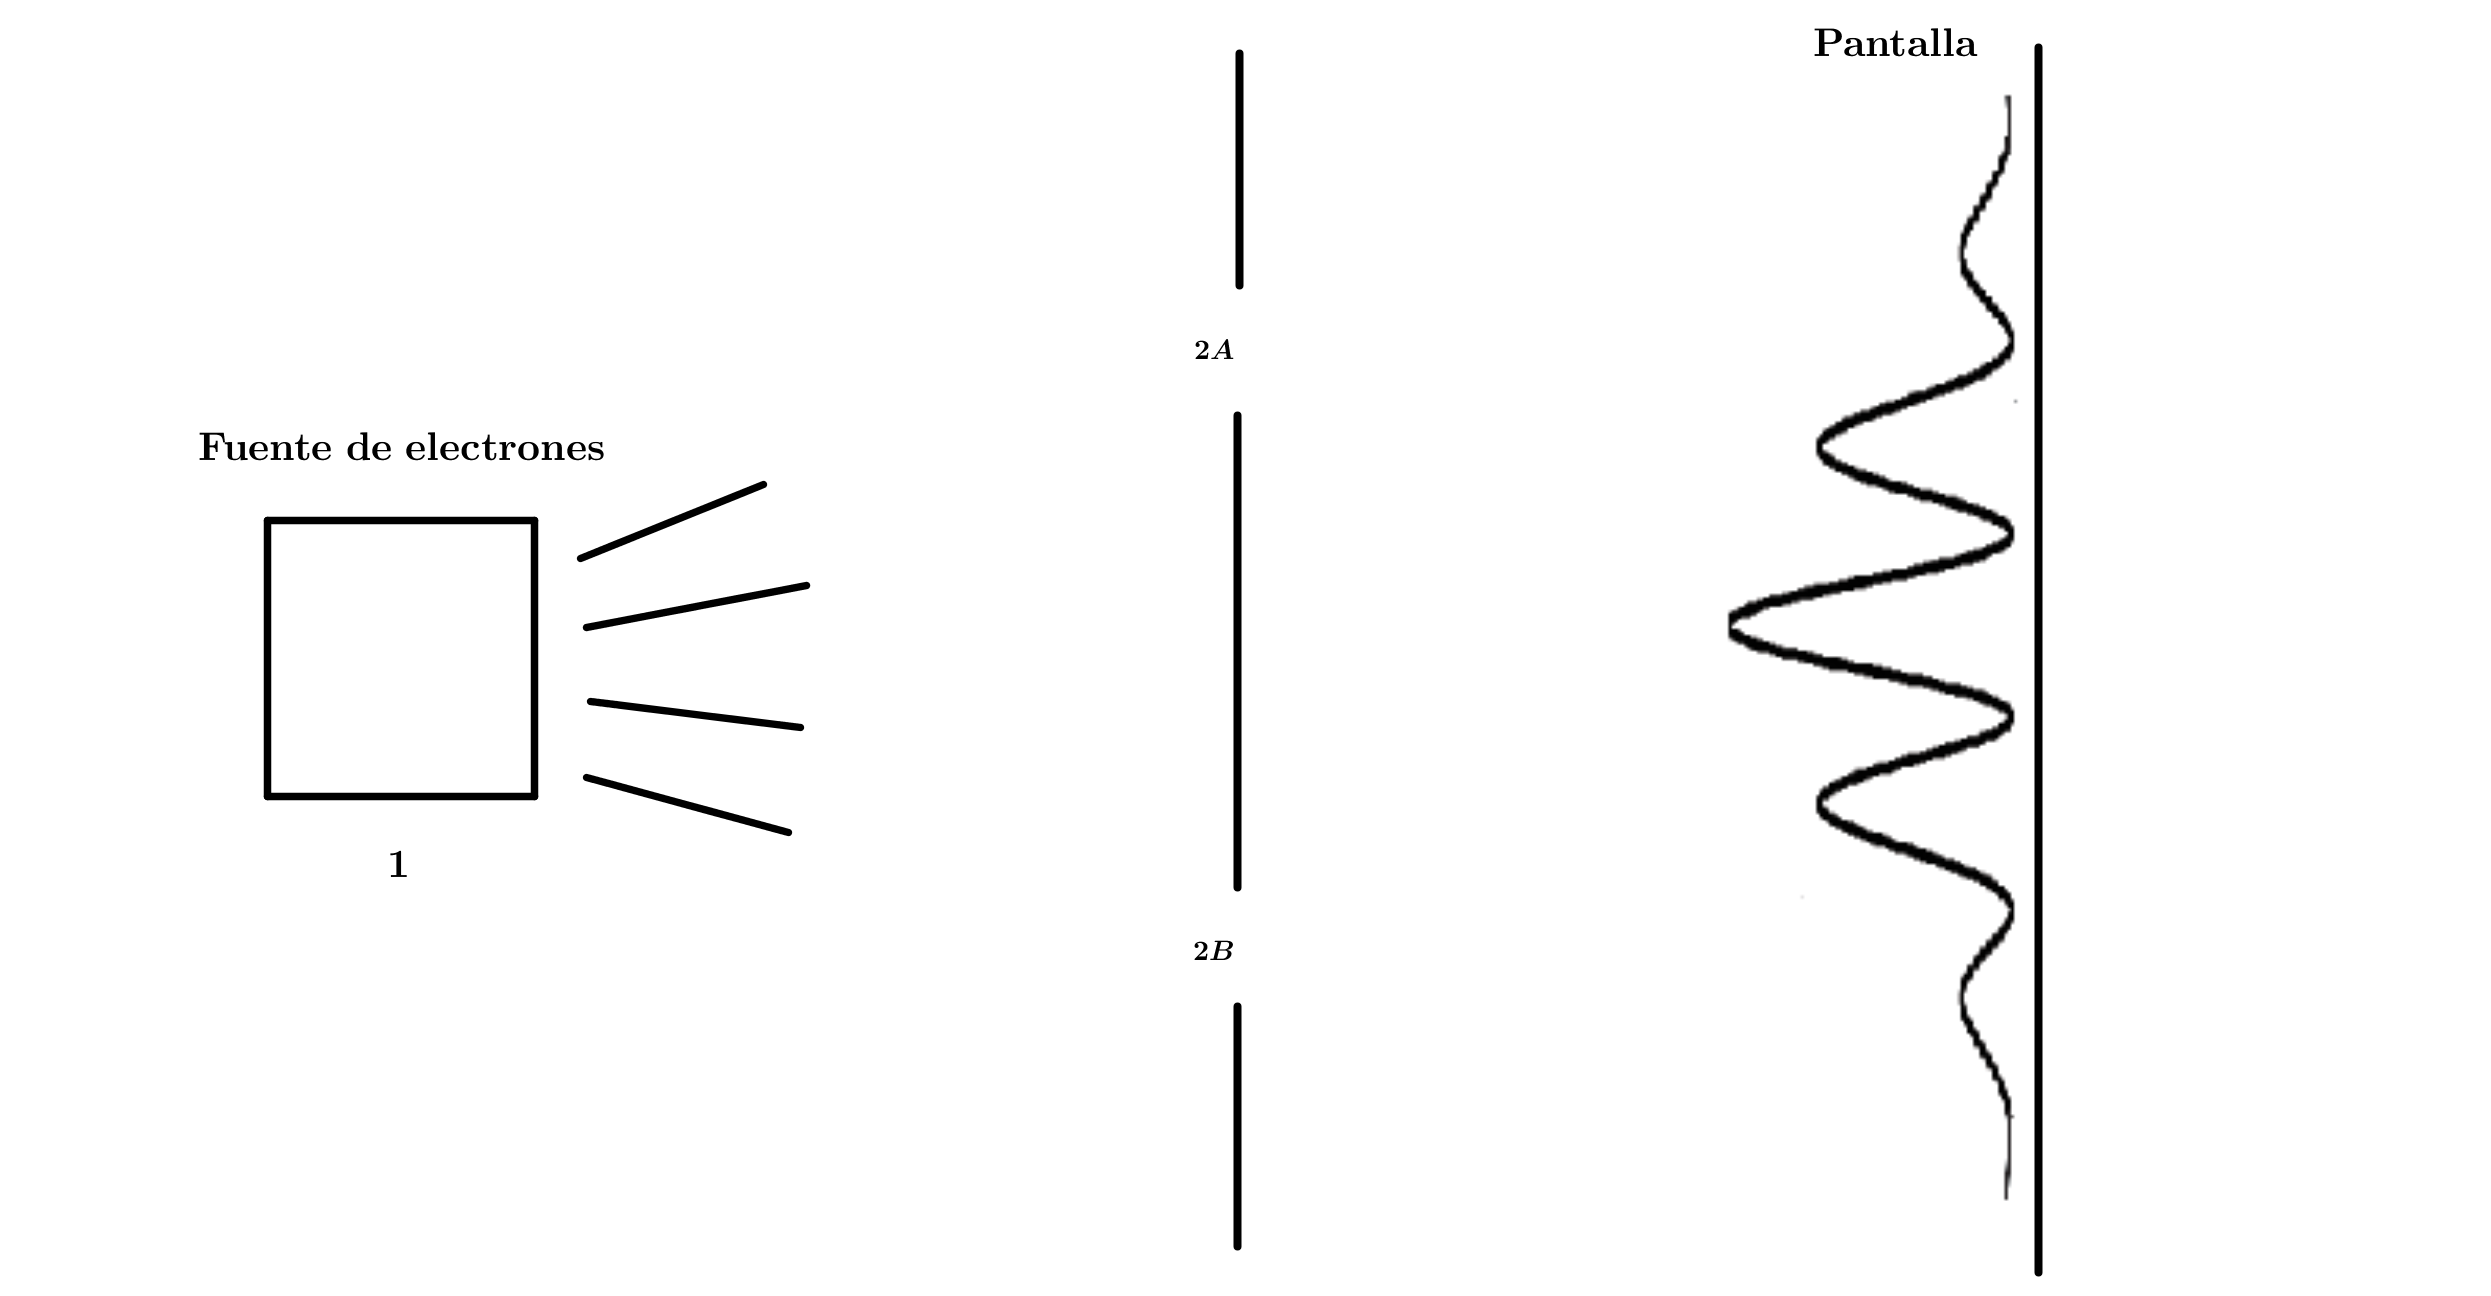
\includegraphics[width=9cm]{Imagenes/Fig1}
\caption[Esquema del experimento de la doble rendija]{Experimento de la doble rendija.}
\end{figure}
si $K(2A,1)$ es la probabilidad de que un electrón pase por la rendija 2A, entonces podemos escribir:
\begin{equation}
K(3,1)=K(2A,1)K(3,2A)+K(2B,1)K(3,2B),
\end{equation}
al tomar el módulo cuadrado de la expresión (2.5) se generarán los términos de interferencia necesarios para describir el patrón de interferencia. No podemos decir que el electrón tomó un camino u el otro, de una manera más simple: este siguió todos los caminos posibles!

\section{La ecuación de Schrödinger.}
En el cuadro de Schrodinger la evolución de un sistema cuántico afecta al ket que representa al estado del sistema [1], la ecuación que rige la dinámica del mismo es la \textbf{Ecuación de Schrödinger}
\begin{equation}
i\hbar\frac{\partial}{\partial t}|\psi\rangle_S=\hat{H}|\psi\rangle_S.
\end{equation}
Sabemos que $\psi(q,t)=\langle q|\psi \rangle_S$ donde $|q\rangle$ son autoestados de la posición, la relacion entre el cuadro de Heisenberg y el de Schrödinger es $|\psi\rangle_H=e^{iHt/\hbar}|\psi\rangle_S$. Si definimos $|qt\rangle \equiv e^{iHt/\hbar}|q\rangle$, entonces $\psi (q,t)=\langle qt|\psi\rangle_H$.

Vamos a mostrar que $K(q_f,t_f;q_i,t_i)=\left\langle q_ft_f|q_it_i \right\rangle$, la relación de completez nos permite escribir:
\begin{eqnarray}
\nonumber \langle q_ft_f|\psi\rangle &=& \int\langle q_ft_f|q_it_i\rangle\langle q_it_i|\psi\rangle dq_i\\
&=& \int \langle q_ft_f|q_it_i\rangle \psi(q_i,t_i)dq_i ,
\end{eqnarray}
y comparando (2.7) y (2.2), vemos que:
\begin{equation}
K(q_f,t_f;q_i,t_i)=\langle q_ft_f|q_it_i\rangle .
\end{equation}
Así, el propagador es proporcional a la amplitud de probabilidad de transición entre el estado inicial $|q_it_i\rangle$ y final $|q_ft_f\rangle$. La idea ahora es expresar el propagador como una integral de trayectoria. Partamos el intervalo temporal $(t_i,t_f)$ en $n+1$ piezas de igual duración $\tau$, así:
\begin{equation}
\langle q_ft_f|q_it_i\rangle = \int dq_1dq_2...dq_n\langle q_ft_f|q_nt_n\rangle \langle q_nt_n|q_{n-1}t_{n-1}\rangle...\langle q_1t_1|q_it_i\rangle .
\end{equation}
Calculemos uno de estos elementos:
\begin{eqnarray}
\nonumber \langle q_{j+1}t_{j+1}|q_jt_j\rangle &=&\langle q_{j+1}|e^{-iHt_{j+1}/\hbar}e^{iHt_j/\hbar}|q_j=\langle q_{j+1}|e^{-i\tau H/\hbar}|q_j\rangle \hspace{0.4cm}\text{A primer orden,}\\
\nonumber &=&\langle q_{j+1}|1-i\tau H/\hbar|q_j\rangle=\delta(q_{j+1}-q_j)-i\tau\hbar\langle q_{j+1}|H|q_j\rangle\\
&=& \frac{1}{2\pi\hbar}\int dp\ \ \exp[\frac{ip}{\hbar}(q_{j+1}-q_j)]-\frac{i\tau}{\hbar}\langle q_{j+1}|H|q_j\rangle , 
\end{eqnarray}	
si asumimos que el Hamiltoniano es una función de $p$ y $q$ de la forma: $H=\frac{p^2}{2m}+V(q)$, entonces:
\begin{eqnarray}
\nonumber \langle q_{j+1}|\frac{p^2}{2m}|q_j \rangle &=& \int dpdp^{\prime} \langle q_{j+1}|p^{\prime}\rangle\langle p^{\prime}|\frac{p^2}{2m}|p\rangle \langle p|q_j \rangle\\
\nonumber &=&\int \frac{dpdp^{\prime}}{2\pi\hbar}\ \ \exp[\frac{i}{\hbar}(p^{\prime} q_{j+1}-pq_j)]\frac{p^2}{2m}\delta(p-p^{\prime})\\
&=& \int \frac{dp}{2\pi\hbar}\ \ \exp[\frac{i}{\hbar}p(q_{j+1}-q_j)]\frac{p^2}{2m} .
\end{eqnarray}
De una manera similar:
\begin{eqnarray}
\nonumber \langle q_{j+1}|V(q)|q_j \rangle &=& V(\frac{q_{j+1}+q_j}{2})\langle q_{j+1}|q_j\rangle\\
\nonumber &=& V(\frac{q_{j+1}+q_j}{2})\delta(q_{j+1}-q_j)\\
\langle q_{j+1}|V(q)|q_j \rangle &=& V(\frac{q_{j+1}+q_j}{2})\int \frac{dp}{2\pi\hbar}\ \ \exp[\frac{i}{\hbar}p(q_{j+1}-q_j)].
\end{eqnarray}
Por tanto $\langle q_{j+1}|H|q_j\rangle=\int \frac{dp}{h}\ \ \exp[\frac{i}{h}p(q_{j+1}-q_j)]H(p,q)$ y :
\begin{equation}
\langle q_{j+1}t_{j+1}|q_jt_j\rangle=\frac{1}{h}\int dp_j\ \ \exp[\frac{i}{\hbar}[p_j(q_{j+1}-q_j)-\tau H(p_j,q_j)]]
\end{equation}
Finalmente:
\begin{equation}
\langle q_{f}t_{f}|q_it_i\rangle=\lim_{N \to \infty}\int\prod_{j=1}^{N}dq_j\prod_{j=0}^{N}\frac{dp_j}{h}\ \ \exp\left\{ \frac{i}{\hbar}\sum_{j=0}^{N}[p_{j}(q_{j+1}-q_{j})-\tau H(p_{j},q_{j})]\right\} ,
\end{equation}
en el continuo:
\begin{equation}
\langle q_{f}t_{f}|q_it_i\rangle=\int\frac{\mathcal{D}q\mathcal{D}p}{h}\ \exp\left\{ \frac{i}{\hbar}\int_{t_{i}}^{t_{f}}(p\dot{q}-H(p,q))dt\right\} . 
\end{equation}
En el continuo $q$ se vuelve una función de $t$ y la integral anterior, es una integral funcional. La expresión (2.15) es la integral de trayectoria para la amplitud de transición entre $(q_i,t_i)$ y $(q_f,t_f)$. Esta integral se hace sobre todas las posibles trayectorias en el espacio de fase y $q(t), p(t)$ son funciones y no operadores, sin embargo es natural preguntarse por la convergencia de (2.15), esto es algo no trivial, sin embargo, de ahora en adelante asumiremos que esta integral existe y converge. 	
\\
Si el Hamiltoniano es tal que $H=\frac{p^2}{2m}+V(q)$
\begin{equation}
\langle q_{f}t_{f}|q_it_i\rangle=\lim_{N \to \infty}\int\prod_{j=1}^{N}dq_j\prod_{j=0}^{N}\frac{dp_j}{h}\ \ \exp\left\{ \frac{i}{\hbar}\sum_{j=0}^{N}[p_{j}(q_{j+1}-q_{j})-\tau \frac{p_j^2}{2m}-V(q)\tau]\right\} ,
\end{equation}
y sabiendo que: $\int_{-\infty}^{\infty}\ \exp[-ax^{2}+bx+c]dx=\ \exp[\frac{b^{2}}{4a}+c](\frac{\pi}{a})^{\frac{1}{2}}$, entonces:
\begin{equation}
\langle q_{f}t_{f}|q_it_i\rangle=\lim_{N\to\infty}[\frac{1}{h}(\frac{\text{\ensuremath{\pi\hbar}2m}}{i\tau})^{\frac{1}{2}}]^{N+1}\int\prod_{1}^{N}dq_{j}\ \exp\left\{ \frac{i}{\hbar}\sum_{0}^{N}\left((\frac{q_{j+1}-q_{j}}{\tau})^{2}\frac{m}{2}-V\right)\tau\right\}. 
\end{equation}
En el continuo:
\begin{equation}
\langle q_{f}t_{f}|q_it_i\rangle=\mathcal{N}\int\mathcal{D}q\ \exp\left\{ \frac{i}{\hbar}\int_{t_{i}}^{t_{f}}\mathcal{L}(q,\dot{q})dt\right\} ,
\end{equation}
donde $\mathcal{L}(q,\dot{q})$ es el lagrangiano clásico, sin embargo, esto solo pasa si asumimos una forma específica del Hamiltoniano, cuando esto no es así se tiene una acción efectiva. En teoría de campos por ejemplo esta descomposición solo se puede hacer en el caso de campos Abelianos.
 
 

\subsection{Teoría de perturbaciones.}

Vamos a ilustrar cómo usar el método de integrales de trayectoria en procesos de dispersión, este tipo de procesos involucran la interacción de una partícula con un potencial $V(x)$. Debido a que no siempre podemos calcular analíticamente la integral (2.18) entonces es necesario acudir a la teoría de perturbaciones, esta es aplicable en el regimen en que la energía de interacción $E_I<\hbar$. En este caso podemos escribir:
\begin{equation}
\ \exp\left[\frac{-i}{\hbar}\int_{t_{i}}^{t_{f}}V(x,t)dt\right]=1-\frac{i}{\hbar}\int_{t_{i}}^{t_{f}}V(x,t)dt+\left(\frac{i}{\hbar}\right)^{2}\frac{1}{2!}\left[\int_{t_{i}}^{t_{f}}V(x,t)dt\right]^{2}+... ,
\end{equation}
cuando reemplazamos esto en la expresión (2.18) obtenemos:
\begin{equation}
K=K_0+K_1+K_2+...\ \text{donde}\ K_0=\mathcal{N}\int \mathcal{D}x \ \exp\left[ \frac{i}{\hbar}\int \frac{1}{2}m\dot{x}^2dt\right] .
\end{equation}
Para calcular $K_0$, escribamos la forma discretizada de (2.20)
\begin{eqnarray}
\nonumber K_0&=&\lim_{n\to\infty}\left(\frac{m}{i\hbar\tau}\right)^{\left(\frac{n+1}{2}\right)}\int_{-\infty}^{\text{\ensuremath{\infty}}}\prod_{j=1}^{n}dx_{j}\ \exp\left[\frac{im}{2\hbar\tau}\sum_{j=0}^{n}\left(x_{j+1}-x_{j}\right)^{2}\right]\\
\nonumber &=& \lim_{n\to\infty}\left(\frac{m}{i\hbar\tau}\right)^{\left(\frac{n+1}{2}\right)}\frac{1}{\left(n+1\right)^{\frac{1}{2}}}\left(\frac{i\hbar\tau}{m}\right)^{\frac{n}{2}}\ \exp\left[\frac{im}{2\hbar(n+1)\tau}\left(x_{f}-x_{i}\right)^{2}\right]\\
K_0(x_ft_f,x_it_i)&=& \Theta(t_{f}-t_{i})\left(\frac{m}{i\hbar(t_{f}-t_{i})}\right)^{1/2}\ \exp\left[\frac{im}{2\hbar(t_{f}-t_{i})}\left(x_{f}-x_{i}\right)^{2}\right] .
\end{eqnarray}
Calculemos ahora $K_1$:
\begin{equation}
K_1=\lim_{n\to\infty}\frac{-i}{\hbar}N^{(n+1)/2}\sum_{i=1}^{n}\int\ \exp\left[\frac{im}{2\hbar\tau}\sum_{j=0}^{n}(x_{j+1}-x_{j})^{2}\right]V(x_{i},t_{i})dx_{1}...dx_{n}.
\end{equation}
Ahora como solo $V(x)$ depende de $x_i$, separamos (2.22) como:
\begin{eqnarray}
\nonumber K_1&=&\lim_{n\to\infty}\frac{-i}{\hbar}\sum_{i=1}^{n}\left\{ \int N^{(n-i+1)/2}\ \exp\left[\frac{im}{2\hbar\tau}\sum_{j=i}^{n}(x_{j+1}-x_{j})^{2}\right]dx_{i}...dx_{n}\right\}\\
& &\times  \left\{ \int N^{i/2}\ \exp\left[\frac{im}{2\hbar\tau}\sum_{j=0}^{i-1}(x_{j+1}-x_{j})^{2}\right]dx_{1}...dx_{i-1}\right\} V(x_{i},t_{i}),
\end{eqnarray}
los dos términos en corchetes en (2.23) son $K_0(xt,x_ft_f)$ y $K_0(x_it_i,xt)$, así:
\begin{equation}
K_1(x_ft_f,x_it_i)= -\frac{i}{\hbar}\int_{t_{i}}^{t_{f}}dt\int_{-\infty}^{\infty}K_{0}(x_{f}t_{f}.xt)V(x,t)K_{0}(xt,x_{i}t_{i})dx .
\end{equation}
Como $K_0(x_ft_f,xt)=0$ si $t>t_f$ y $K_0(xt,x_it_i)=0$ si $t<t_i$, entonces podemos escribir:
\begin{equation}
K_1(x_ft_f,x_it_i)=-\frac{i}{\hbar}\int_{-\infty}^{\infty}dt\int_{-\infty}^{\infty}K_{0}(x_{f}t_{f}.xt)V(x,t)K_{0}(xt,x_{i}t_{i})dx .
\end{equation}
De la misma manera se puede probar que:
\begin{equation}
K_2(x_ft_f,x_it_i)=\left(\frac{-i}{\hbar}\right)^2\int_{-\infty}^{\infty}dt_{1}dt_{2}dx_{1}dx_{2}K_{0}(x_{f}t_{f}.x_{2}t_{2})V_2K_{0}(x_{2}t_{2},x_{1}t_{1})V_1K_{0}(x_{1}t_{1},x_{i}t_{i}).
\end{equation}
Esta es una solución en series para $K$ y recibe el nombre de Serie de Born, en la expresión general para $K_n$ no se tiene el factor $n!$ ya que hay ese mismo numero de formas para ordenar los $n$ potenciales $V(x)$ que entran en el propagador.
\\
\\
Por último mostraremos que \textbf{el propagador es la función de Green de la ecuación de Schrödinger.} Para esto sustituyamos la expresión para la serie de Born en la ecuación (2.2):
\begin{eqnarray}
\nonumber \psi(\vec{x}_f,t_f)&=&\int K_{0}(\vec{x_{f}}t_{f},\vec{x_{i}}t_{i})\psi(\vec{x_{i}},t_{i})d\vec{x_{i}}\\
& & \frac{-i}{\hbar}\int K_{0}(\vec{x_{f}}t_{f},\vec{x}t)V(\vec{x},t)K_{0}(\vec{x}t,\vec{x_{i}}t_{i})\psi(\vec{x_{i}},t_{i})d\vec{x}dtd\vec{x_{i}}+O(\hbar^{2}),
\end{eqnarray}
hemos cambiado a tres dimensiones espaciales y los otros términos en la serie hacen converger el último $K_0$ a $K$, por tanto:
\begin{equation}
\psi(\vec{x}_f,t_f)=\int K_{0}(\vec{x_{f}}t_{f},\vec{x_{i}}t_{i})\psi(\vec{x_{i}},t_{i})d\vec{x_{i}}-\frac{i}{\hbar}\int K_{0}(\vec{x_{f}}t_{f},\vec{x}t)V(\vec{x},t)\psi(\vec{x},t)d\vec{x}dt .
\end{equation}
Cuando $t_i \to -\infty$,no hay presencia de potencial por tanto $\psi$ se vuelve una onda plana. Así:
\begin{equation}
\psi(\vec{x}_f,t_f)=\phi(\vec{x}_ft_f)-\frac{i}{\hbar}\int K_{0}(\vec{x_{f}}t_{f},\vec{x}t)V(\vec{x},t)\psi(\vec{x},t)d\vec{x}dt.
\end{equation}
Aplicando el operador $\hat{H}=\frac{\hbar^2}{2m}\nabla_{\vec{x}_ft_f}+i\hbar\frac{\partial}{\partial t_f}$ en la ecuación (donde $\nabla_{\vec{x}_ft_f}$ denota diferenciación respecto a $\vec{x}_ft_f$ )(2.29) y usando $\hat{H}\psi(x,t)=V(x,t)\psi(x,t)$:
\begin{eqnarray}
\nonumber \hat{H}(\psi(\vec{x}_f,t_f))&=&\hat{H}(\phi(\vec{x}_ft_f))-\frac{i}{\hbar}\int\hat{H} (K_{0}(\vec{x_{f}}t_{f},\vec{x}t))V(\vec{x},t)\psi(\vec{x},t)d\vec{x}dt\\
\nonumber V(\vec{x}_f,t_t)\psi(\vec{x}_f,t_f)&=&0-\frac{i}{\hbar}\int\hat{H} (K_{0}(\vec{x_{f}}t_{f},\vec{x}t))V(\vec{x},t)\psi(\vec{x},t)d\vec{x}dt ,
\end{eqnarray}
por tanto:
\begin{equation}
\left(\frac{\hbar^2}{2m}\nabla_{\vec{x}_ft_f}+i\hbar\frac{\partial}{\partial t_f}\right)K_{0}(\vec{x_{f}}t_{f},\vec{x}t)=i\hbar\delta(\vec{x}-\vec{x}_f)\delta(t-t_f).
\end{equation}
Esto último era lo que queríamos probar.








\subsection{Matriz $\mathcal{S}$.}
En un experimento de dispersión es razonable suponer que las partículas al principio y al final del proceso son partículas libres, estas ondas planas están distribuidas en todo el espacio. Sin embargo, esto último lleva a una contradicción ya que la presencia del centro dispersor no permite que en sus cercanias la solución sea una onda plana. Para resolver este inconveniente se puede proponer lo que se llama una fuente dinámica, que se "prenda y apague" lentamente tal que las partículas en los estados (final/incial) puedan ser libres y por tanto la aproximación de ondas planas sea válida en este regimen.\\
\\
Para empezar definamos $\psi_{in}(\vec{x}_i,t_i)$, $\psi_{out}(\vec{x}_f,t_f)$ como ondas planas para $t\to -\infty$,  $t\to \infty$ respectivamente, la amplitud de dispersión se define como:
\begin{equation}
\mathcal{S}=\int\psi_{out}^{*}(\vec{x}_{f}t_{f})\psi^{(+)}(\vec{x}_{f}t_{f})d\vec{x}_{f}.
\end{equation}
En (2.31) el superíndice $(+)$ denota que $\psi^{(+)}(\vec{x}t)$ era una onda libre en $t\to -\infty$, usando la serie de Born obtenemos:
\begin{eqnarray}
\nonumber \mathcal{S}&=&\int\psi_{out}^{*}(\vec{x}_{f}t_{f})\psi^{(+)}(\vec{x}_{f}t_{f})d\vec{x}_{f}=\int\psi_{out}^{*}(\vec{x}_{f}t_{f})K_{0}(\vec{x}_{f}t_{f},\vec{x}_{i}t_{i})\psi_{in}(\vec{x}_{i}t_{i})d\vec{x}_{f}d\vec{x_{i}}\\
\nonumber &&-\frac{i}{\hbar}\int\psi_{out}^{*}(\vec{x}_{f}t_{f})K_{0}(\vec{x}_{f}t_{f},\vec{x}t)V(\vec{x}t)K_{0}(\vec{x}t,\vec{x}_{i}t_{i})\psi_{in}(\vec{x}_{i}t_{i})d\vec{x}_{f}d\vec{x_{i}}d\vec{x}dt\\
\nonumber &=&\int \psi_{out}^{*}(\vec{x}_{f}t_{f})\phi(\vec{x}_{f}t_{f})d\vec{x}_f\\
&&-\frac{i}{\hbar}\int\psi_{out}^{*}(\vec{x}_{f}t_{f})K_{0}(\vec{x}_{f}t_{f},\vec{x}t)V(\vec{x}t)K_{0}(\vec{x}t,\vec{x}_{i}t_{i})\psi_{in}(\vec{x}_{i}t_{i})d\vec{x}_{f}d\vec{x_{i}}d\vec{x}dt.   
\end{eqnarray}
Si los momentos iniciales y finales son $\vec{p}_i=\hbar\vec{k}_i$,$\vec{p}_f=\hbar\vec{k}_f$ respectivamente, entonces tenemos que:
\begin{eqnarray}
\psi_{in}(\vec{x}t)&=&\frac{1}{\sqrt{\tau}}\ \exp\left( \frac{i}{\hbar}(\vec{p}_i\cdot \vec{x}-E_it )\right)\\
\psi_{out}(\vec{x}t)&=&\frac{1}{\sqrt{\tau}}\ \exp\left( \frac{i}{\hbar}(\vec{p}_f\cdot \vec{x}-E_ft )\right),
\end{eqnarray}
donde $E^2=\frac{p^2}{2m}$ y $\tau$ es el volumen de integración, el cual es arbitrario. Si sustituimos las expresiones (2.33) y (2.34) en (2.32) obtenemos:
\begin{equation}
\mathcal{S}_{fi}=\delta(\vec{k}_f-\vec{k}_i)-\frac{i}{\hbar}\int\psi_{out}^{*}(\vec{x}_{f}t_{f})K_{0}(\vec{x}_{f}t_{f},\vec{x}t)V(\vec{x}t)K_{0}(\vec{x}t,\vec{x}_{i}t_{i})\psi_{in}(\vec{x}_{i}t_{i})d\vec{x}_{f}d\vec{x_{i}}d\vec{x}dt.
\end{equation}
Lo cual nos permite ver la amplitud de dispersion $\mathcal{S}_{fi}$ como el elemento de una matriz, la \textbf{matriz $\mathcal{S}$ de dispersión}. En (2.35) el primer término solo es representativo cuando no hay interacción y $\vec{k}_i=\vec{k}_f$. Las interacciones están representadas en el segundo término.\\
\\
Es posible representar este segundo término mediante una serie de diagramas a los cuales se les asocian ciertas reglas, estos diagramas reciben el nombre de \textbf{Diagramas de Feynmann}. Si nombramos:
\begin{equation}
\mathcal{A}=-\frac{i}{\hbar}\int\psi_{out}^{*}(\vec{x}_{f}t_{f})K_{0}(\vec{x}_{f}t_{f},\vec{x}t)V(\vec{x}t)K_{0}(\vec{x}t,\vec{x}_{i}t_{i})\psi_{in}(\vec{x}_{i}t_{i})d\vec{x}_{f}d\vec{x_{i}}d\vec{x}dt,
\end{equation}

\begin{SCfigure}[1.3][h]
\caption[Diagrama de Feynmann primera cuantización]{Representación de $\mathcal{A}$.}
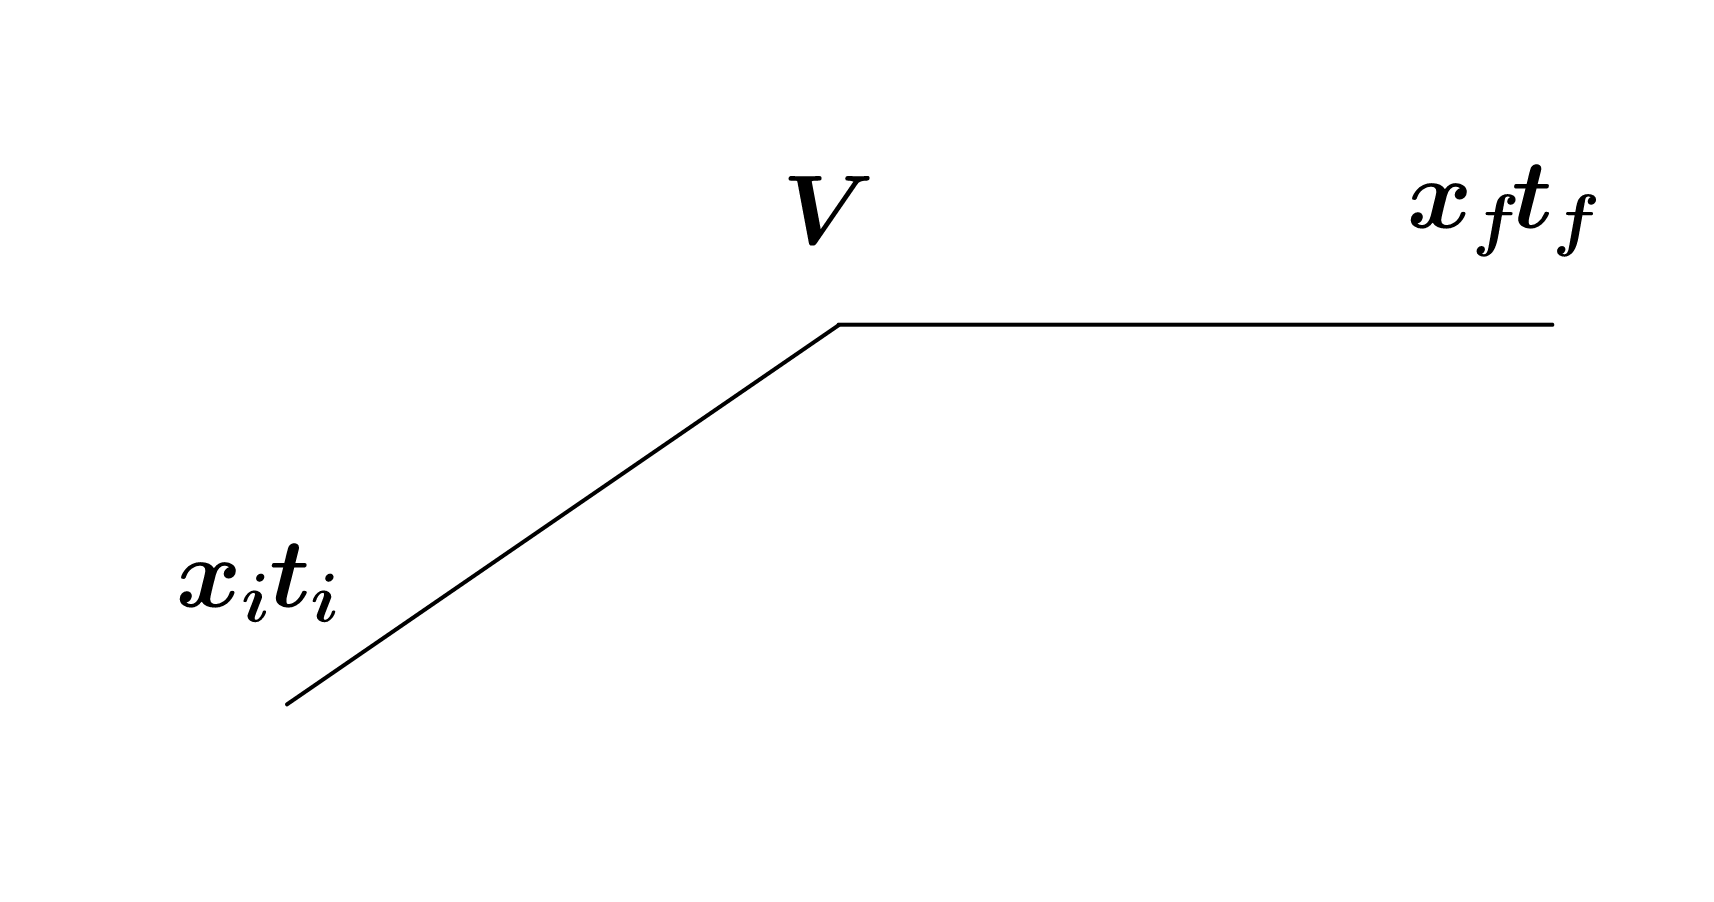
\includegraphics[width=4cm]{Imagenes/Fig2}
\end{SCfigure}
este diagrama lo podemos descomponer usando la siguiente convención:
\begin{SCfigure}[1.3][h]
\caption[Diagrama de Feynmann primera cuantización]{Representación de $K_0(x_2t_2,x_1t_1)$.}
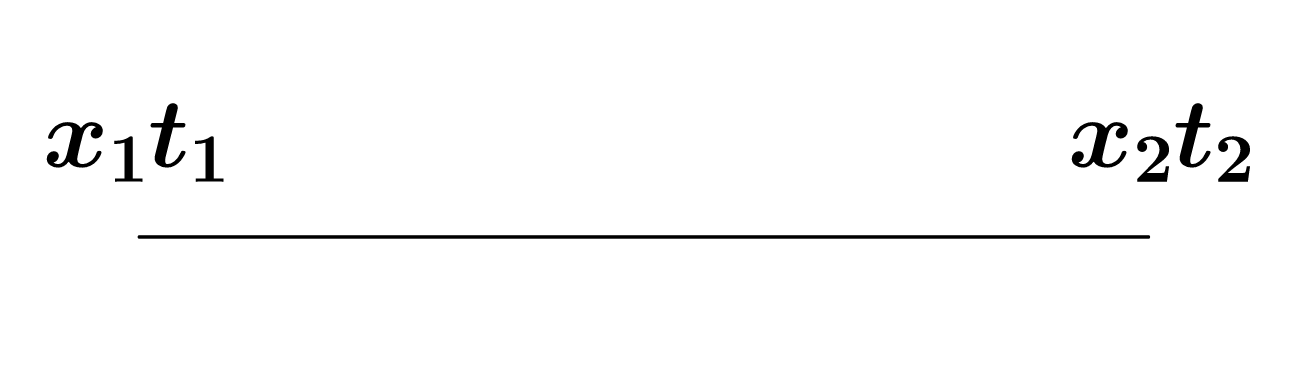
\includegraphics[width=4cm]{Imagenes/Fig3}
\end{SCfigure}
\begin{SCfigure}[1.3][h]
\caption[Diagrama de Feynmann primera cuantización]{Representación de $\int -\frac{i}{\hbar}V(xt)dxdt$.}
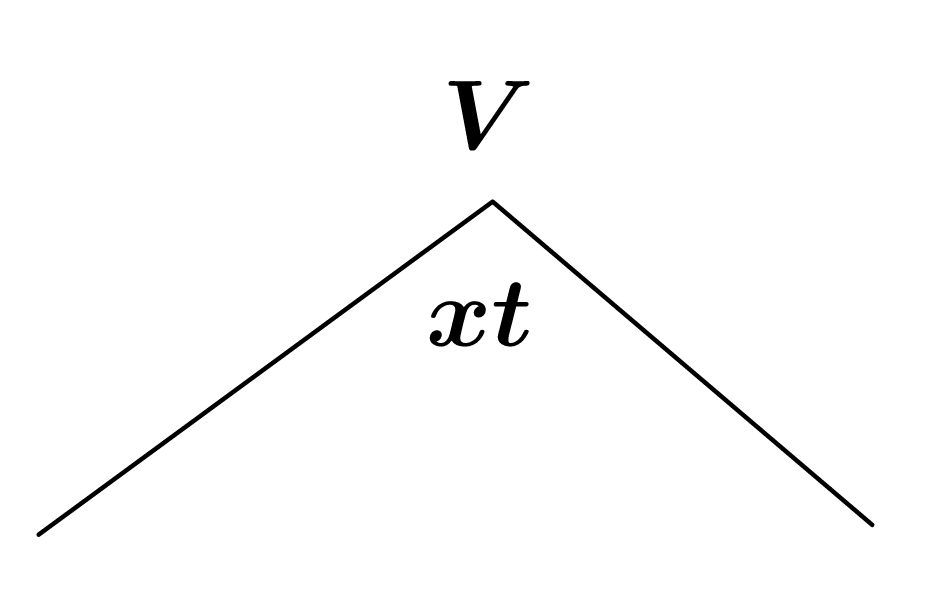
\includegraphics[width=4cm]{Imagenes/Fig4}
\end{SCfigure}
\\
Por ejemplo el diagrama correspondiente a término de segundo orden:
\begin{eqnarray}
\nonumber \mathcal{A}^{(2)}&=&\left(-\frac{i}{\hbar}\right)^2\int d\vec{x}_{f}d\vec{x_{i}}d\vec{x^{\prime}}dt^{\prime} d\vec{x}dtK_{0}(\vec{x}t,\vec{x}_it_i)V(\vec{x}t)K_{0}(\vec{x}^{\prime} t^{\prime},\vec{x}t)\\
&&\times V(\vec{x}^{\prime} t^{\prime})K_{0}(\vec{x}_{f}t_{f},\vec{x}^{\prime} t^{\prime})\psi_{out}^{*}(\vec{x}_{f}t_{f})\psi_{in}(\vec{x}_{i}t_{i}),
\end{eqnarray}
es el que se muestra enm la figura 2.5 .
\begin{SCfigure}[1.3][h]
\caption[Diagrama de Feynmann primera cuantización]{Representación de $\mathcal{A}^{(2)}$}
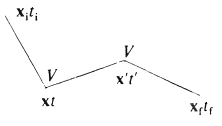
\includegraphics[width=4cm]{Imagenes/Fig5}
\end{SCfigure}
\\
\\
En algunos casos es útil conocer una expresión para el propagador  $K_0$ en el espacio de momentos, definimos $\mathcal{K}_0(\vec{p}_1t_1,\vec{p}_2t_2)$ como la amplitud de que una partícula con momento $\vec{p}_2$ en un instante $t_2$, sea observada un instante de tiempo después en $t_1$ con momento $\vec{p}_1$. Así:
\begin{eqnarray}
\nonumber \mathcal{K}_0(\vec{p}_1t_1,\vec{p}_0t_0)&=&\int \ \exp\left(\frac{-i}{\hbar}(\vec{p}_1\cdot\vec{x}_1)\right) K_0(\vec{x}_1t_1,\vec{x}_0t_0)\ \exp\left(\frac{-i}{\hbar}(\vec{p}_0\cdot\vec{x}_0)\right)d\vec{x}_0d\vec{x}_1\\
&&\nonumber \Theta(t_{1}-t_{0})\left(\frac{m}{i\hbar(t_{1}-t_{0})}\right)^{1/2}\int\ \exp\left[\frac{i}{\hbar}(\vec{p}_{0}\cdot\vec{x}_{0}-\vec{p}_{1}\cdot\vec{x}_{1})\right]\\
&& \times \ \exp\left[\frac{im(\vec{x}_{0}-\vec{x}_{1})^{2}}{2\hbar(t_{1}-t_{0})}\right]d\vec{x}_{0}d\vec{x}_{1},
\end{eqnarray}
ahora si introducimos las siguientes variables:
\begin{equation}
\vec{x}=\vec{x}_0-\vec{x}_1;\hspace{0.3cm}\vec{X}=\vec{x}_0+\vec{x}_1;\hspace{0.3cm}\vec{p}=\vec{p}_0-\vec{p}_1;\hspace{0.3cm}\vec{P}=\vec{p}_0+\vec{p}_1 ,
\end{equation}
teniendo en cuenta que el Jacobiano de esta transformación es $J=\left(\frac{1}{2}\right)^3=\frac{1}{8}$ y con $\alpha=\frac{m}{2\hbar (t_1-t_0)}$  podemos escribir:
\begin{equation}
\mathcal{K}_0(\vec{p}_1t_1,\vec{p}_0t_0)=\Theta(t_{1}-t_{0})\left(\frac{\alpha}{i\pi}\right)^{3/2}\frac{1}{8}\int\ \exp\left[\frac{i\vec{p}\cdot\vec{X}}{2\hbar}\right]d\vec{X}\int\ \exp\left[\frac{i\vec{P}\cdot\vec{x}}{2\hbar)}\right]e^{i\alpha x^{2}}d\vec{x}.
\end{equation}
La primera integral es $I_1=8(2\pi\hbar)^3\delta(\vec{p}_0-\vec{p}_1)$, la segunda la podemos calcular con la identidad $ \int e^{-ax^2+bx+c}=e^{\frac{b^2}{4a}+c}\left(\frac{\pi}{a}\right)^(1/2)$, por tanto $I_2=\left(\frac{i\pi}{\alpha}\right)^{3/2}\ \exp\left[\frac{-i\vec{P}^{2}}{8\hbar^{3}4i\alpha}\right]$, por tanto:
\begin{equation}
\mathcal{K}_0(\vec{p}_1t_1,\vec{p}_0t_0)=(2\pi\hbar)^3\Theta(t_1-t_0)\delta(\vec{p}_1-\vec{p}_0)\ \exp\left[\frac{-i\vec{P}^{2}(t_{1}-t_{0})}{8m\hbar}\right].
\end{equation}
Si también realizamos la transformada de Fourier en el tiempo, obtenemos:
\begin{equation}
\mathcal{K}_0(\vec{p}_1E_1,\vec{p}_0E_0)=(2\pi\hbar)^4\delta(\vec{p}_0-\vec{p}_1)\delta(E_1-E_0)\frac{i\hbar}{E-\frac{p_{1}^{2}}{2m}+i\epsilon}.
\end{equation}
De lo anterior las reglas de Feynmann en el espacio de momentos son:
\begin{SCfigure}[1.3][h]
\caption[Diagrama de Feynmann primera cuantización]{Representación de $\frac{1}{(2\pi\hbar)^4}\frac{i\hbar}{E-\frac{p_{1}^{2}}{2m}+i\epsilon}$}
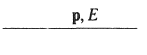
\includegraphics[width=4cm]{Imagenes/Fig6}
\end{SCfigure}
\begin{SCfigure}[1.3][h]
\caption[Diagrama de Feynmann primera cuantización]{Representación de $\frac{-i}{\hbar}(2\pi\hbar)^4v(\vec{q},W)$}
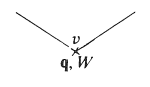
\includegraphics[width=4cm]{Imagenes/Fig7}
\end{SCfigure}

\subsection{Propiedades adicionales de las integrales de trayectoria.}
Ya hemos mostrado que la amplitud de transición entre un estado $(q_i,t_i)$ a $(q_f,t_f)$ está dada por:
\begin{equation}
\langle q_{f}t_{f}|q_it_i\rangle=\mathcal{N}\int\mathcal{D}q\text{Exp\ensuremath{\left\{ \frac{i}{\hbar}\int_{t_{i}}^{t_{f}}\mathcal{L}(q,\dot{q})dt\right\} }}.
\end{equation}
En un experimento real, las partículas creadas en algún instante en el pasado son destruidas al ser detectadas, esto lo podemos interpretar de la siguiente manera: El estado de vacío en $t=-\infty$ evoluciona al mismo vacío en $t=\infty$. En este proceso una partícula es creada para ser posteriormente destruida, todo esto en presencia de una fuente generadora de estos procesos. Así es razonable poner nuestro interés en calcular transiciones vacío-vacío en presencia de una fuente.\\
\\
Podemos modificar el Lagrangiano de la de la siguiente manera: $\mathcal{L} \to \mathcal{L}+\hbar J(t)q(t)$. Si $|0,t\rangle^J $ es el estado fundamental en presencia de la fuente, entonces la amplitud de transición se define de la siguiente manera:
\begin{equation}
Z[J]\propto \langle 0,\infty|0,-\infty\rangle ^J.
\end{equation}
La fuente $J(t)=0$ para $t>t^{\prime}$ , $t^{\prime} < t$. Instroduzcamos entonces $T$ y $T^{\prime} $ de tal manera que $T<t^{\prime} $ , $T^{\prime}>t^{\prime} $ por tanto la amplitud (2.44) es:
\begin{equation}
\langle 	Q^{\prime} T^{\prime} |QT\rangle=\mathcal{N}\int\mathcal{D}q\text{Exp\ensuremath{\left\{ \frac{i}{\hbar}\int_{T}^{T^{\prime}}\mathcal{L}(q,\dot{q})dt\right\} }},
\end{equation}
podemos escribir:
\begin{equation}
\langle Q^{\prime} T^{\prime} |QT \rangle^J=\int dq^{\prime} dq\langle Q^{\prime} T^{\prime} | q^{\prime} t^{\prime}  \rangle\langle q^{\prime} t^{\prime} | qt \rangle\langle qt|QT \rangle .
\end{equation}
Ahora si denotamos $|E_q\rangle$ como un autoestado del hamiltoniano podemos usar estos estados para expandir:
\begin{eqnarray}
\nonumber \langle Q^{\prime} T^{\prime} | q^{\prime} t^{\prime}  \rangle &=& \langle Q\prime|\ \exp\left[\frac{-i}{\hbar}HT^{\prime}\right]\ \exp\left[\frac{i}{\hbar}Ht^{\prime}\right]|q^{\prime}\rangle\\
\nonumber &=& \sum_{mn}\phi^{*}(q^{\prime})\phi(Q^{\prime})\langle E_{Q^{\prime}}|\ \exp\left[\frac{-i}{\hbar}HT^{\prime}\right]\ \exp\left[\frac{i}{\hbar}Ht^{\prime}\right]|E_{q^{\prime}}\rangle\\
&=&\sum_{m}\phi^{*}(q^{\prime})\phi(Q^{\prime}) \exp\left[\frac{i}{\hbar}E_{m}(t^{\prime}-T^{\prime})\right],
\end{eqnarray}
de la misma manera:
\begin{equation}
\langle qt|	QT  \rangle=\sum_{m}\phi^{*}(Q)\phi(q)\ \exp\left[\frac{i}{\hbar}E_{m}(t-T)\right].
\end{equation}
Introduciendo (2.47) y (2.48) en (2.46):
\begin{eqnarray}
\nonumber \langle Q^{\prime} T^{\prime}|QT\rangle &=&\int dq^{\prime} dq\sum_{m}\phi_{m}(Q^{\prime})\phi_{m}(q^{\prime},t)\ \exp\left[\frac{-i}{\hbar}E_{m}T^{\prime}\right]\\
&&\times  \sum_{n}\phi_{n}^{*}(Q)\phi_{n}^{*}(q,t)\ \exp\left[\frac{i}{\hbar}E_{n}T\right]\langle q^{\prime} t^{\prime}|qt\rangle^{J}.
\end{eqnarray}
Si hacemos una rotación de Wick de $T$ y $T^{\prime} $ nos damos cuenta que el término que menos sufre de supresión en la integral (2.49) es el asociado a $m=n=0$, por tanto:
\begin{equation}
\int dq^{\prime} dq\phi_{0}^{*}(q^{\prime},t^{\prime})\langle q^{\prime} t^{\prime}|qt\rangle^{J}\phi_{0}(q,t)=\lim_{T\to-\text{\ensuremath{\infty}e}^{-i\delta},T^{\prime}\to\text{\ensuremath{\infty}e}^{-i\delta}}\frac{\langle Q^{\prime} T^{\prime}|QT\rangle^{J}}{\phi_{0}^{*}(Q)\phi_{0}(Q^{\prime})\ \exp\left[\frac{-i}{\hbar}E_{0}(T^{\prime}-T)\right]}.
\end{equation}
El RHS de (2.50) es simplemente el valor de expectación en el vacio de la amplitud de transcición, justo lo que buscabamos y el denominador de la parte derecha de la ecuación es simplemente una constante, así:
\begin{equation}
\langle 0,\infty| 0,-\infty \rangle ^J \propto \lim_{T\to-\text{\ensuremath{\infty}e}^{-i\delta},T^{\prime}\to\text{\ensuremath{\infty}e}^{-i\delta}}\langle Q^{\prime} T^{\prime}|QT\rangle^{J}.
\end{equation}
Otra forma equivalente de obtener este mismo resultado es: en vez de hacer una rotación de Wick, podemos agregar una pequeña cantidad imaginaria negativa al hamiltoniano $H+(-\frac{1}{2}i\epsilon q^2)$, lo cual es equivalente a restar esta misma cantidad a $\mathcal{L}$, de aquí que:
\begin{equation}
Z[J]=\int\mathcal{D}q\ \exp\left\{ \frac{i}{\hbar}\int_{-\infty}^{\infty}(\mathcal{L}(q,\dot{q})+\hbar Jq + \frac{1}{2}i\epsilon q^2)dt\right\} .
\end{equation}
En general se cumple que:
\begin{equation}
 \langle q_{f}t_{f}|T[q(t_{1})...q(t_{n})]|q_{i}t_{i}\rangle=\mathcal{N}\int\mathcal{D}qq(t_{1})...q(t_{n})\ \exp\left[\frac{i}{\hbar}\int_{t_{i}}^{t_{f}}\mathcal{L}dt\right],
\end{equation}
donde $T$ es el operador de ordenamiento temporal. Si derivamos funcionalmente la expresión para $Z[J]$ respecto a $J(t)$ obtenemos:
\begin{equation}
\frac{\delta Z[J]}{\delta J(t_{1}).}|_{J=0}=i\mathcal{N}\int\mathcal{D}qq(t_{1})\ \exp\left[\frac{i}{\hbar}\int_{t_{i}}^{t_{f}}\mathcal{L}dt\right],
\end{equation}	
haciendo esto $n$ veces:
\begin{equation}
\frac{\delta^{n}Z[J]}{\delta J(t_{1})...\delta J(t_{n}).}|_{J=0}=i^{n}\mathcal{N}\int\mathcal{D}qq(t_{1})...q(t_{n})\ \exp\left[\frac{i}{\hbar}\int_{t_{i}}^{t_{f}}\mathcal{L}dt\right].
\end{equation}
De igualar las ecuaciones (2.53), (2.55) y al tener en cuenta agregar el factor $\frac{1}{2}i\epsilon q^2$ (el cual simplemente va a hacer converger los estados inicial y final en (2.53) a estados de vacío) obtenemos:
\begin{equation}
\frac{\delta^{n}Z[J]}{\delta J(t_{1})...\delta J(t_{n}).}|_{J=0}\propto i^{n}\langle0,\infty|T[q(t_{1})...q(t_{n})]|0,-\infty\rangle .
\end{equation}
Estas últimas expresiones que hemos derivado van a ser importantes como punto de partida a la hora de tratar de cuantizar una teoría de campos vía el formalismo de integrales de trayectoria.
\newpage


\section{El experimento de la doble rendija.}
En esta sección aplicaremos lo aprendido en la $\mathsection$2.1 para resolver vía integrales de trayectoria el conocido problema de la difracción de electrones por una y dos rendijas. 

\subsection{El propagador de una partícula libre.}

Con este objetivo en mente primero necesitamos conocer el propagador de una partícula libre, sabemos que en un espacio plano de una dimensión la integral de trayectoria está dada por la expresión (2.17),podemos hacer fácilmente una analogía para un espacio euclídeo d-dimensional. En este caso el propagador es:
\begin{eqnarray}
\nonumber K(x_{f}t_{f,},x_{i,}t_{i})&=&\lim_{n\to\infty}\frac{1}{(2\pi i\hbar\epsilon/m)^{d/2}}\prod_{k=1}^{n}\int\frac{d^{d}x_{k}}{(2\pi i\hbar\epsilon/m)^{d/2}}\\
&&\times \ \exp\left\{ \frac{i}{\hbar}\sum_{k=1}^{n}\epsilon\left[\frac{m(x_{k}-x_{k-1})^{2}}{2\epsilon^{2}}-V(x_{k})\right]\right\}, 
\end{eqnarray}
donde $\epsilon=(t_i-t_f)/n$; para una partícula libre $V(x_k)=0$, entonces:
\begin{equation}
K(x_{f}t_{f,},x_{i,}t_{i})=\lim_{n\to\infty}\frac{1}{(2\pi i\hbar\epsilon/m)^{d/2}}\prod_{k=1}^{n}\int\frac{d^{d}x_{k}}{(2\pi i\hbar\epsilon/m)^{d/2}}\ \exp\left\{ \frac{i}{\hbar}\sum_{k=1}^{n}\left[\frac{m(x_{k}-x_{k-1})^{2}}{2\epsilon}\right]\right\}.
\end{equation}
Para $d=1$, integremos los términos que tienen que ver con $x_1$:
\begin{eqnarray}
\nonumber &\frac{1}{(2\pi i\hbar\epsilon/m)^{1/2}}\prod_{k=1}^{n}\int\frac{dx_{1}}{(2\pi i\hbar\epsilon/m)^{1/2}}\ \exp\left\{ \frac{im(x_{1}-x_{0})^{2}}{2\hbar\epsilon}\right\} \ \exp\left\{ \frac{im(x_{2}-x_{1})^{2}}{2\hbar\epsilon}\right\}\\
\nonumber &=\frac{1}{(2\pi i\hbar\epsilon/m)}\int dx_{1}\ \exp\left\{ \frac{-m}{2i\epsilon\hbar}\left(2x_{1}^{2}-2x_{1}(x_{2}+x_{0})+x_{0}^{2}+x_{2}^{2}\right)\right\}\\
\nonumber &\text{Usando} \ \int e^{-ax^{2}+bx+c}dx=e^{^{\frac{b^{2}}{4a}+c}}\left(\frac{\pi}{a}\right)^{1/2}\\
\nonumber &=\frac{1}{\sqrt{2\pi i\hbar(2\epsilon)/m}}\ \exp\left\{ \frac{im(x_{2}-x_{0})^{2}}{2\hbar(2\epsilon)}\right\}, 
\end{eqnarray}
ahora al seguir con la integral de $x_2$ queda:
\begin{eqnarray}
\nonumber & \frac{1}{(2\pi i\hbar\epsilon/m)\sqrt{2}}\int dx_{2}\ \exp\left\{ \frac{im}{2\hbar(2\epsilon)}\left(x_{2}-x_{o}\right)^{2}\right\} \ \exp\left\{ \frac{im}{2\hbar\epsilon}\left(x_{3}-x_{2}\right)^{2}\right\} \\
&=\frac{1}{\sqrt{2\pi i\hbar(3\epsilon)/m}}\ \exp\left\{ \frac{im(x_{3}-x_{0})^{2}}{2\hbar(3\epsilon)}\right\}. 
\end{eqnarray}
Así, por inducción:
\begin{eqnarray}
\nonumber K(x_{f}t_{f},x_{i}t_{i})&=&\lim_{n\to\infty}\frac{1}{\sqrt{2\pi i\hbar(n\epsilon)/m}}\ \exp\left\{ \frac{im(x_{f}-x_{i})^{2}}{2\hbar(n\epsilon)}\right\} \\
&=& \frac{1}{\sqrt{2\pi i\hbar(t_{f}-t_{i})/m}}\ \exp\left\{ \frac{im(x_{f}-x_{i})^{2}}{2\hbar(t_{f}-t_{i})}\right\} .
\end{eqnarray}
Por tanto en 3-D:
\begin{equation}
K^{3D}(x_{f}t_{f},x_{i}t_{i})\equiv K_{0}^{3D}=\left(\frac{m}{2\pi i\hbar(t_{f}-t_{i})}\right)^{3/2}\ \exp\left\{ \frac{im|\vec{x}_{f}-\vec{x}_{i}|^{2}}{2\hbar(t_{f}-t_{i})}\right\} .
\end{equation}


\subsection{El problema de difracción e interferencia.}
Consideremos el siguiente experimento: una fuente de electrones en $(x,y,z)=(0,0,0)$ y dos rendijas en $Z=D$ con ancho $2a$ y centradas en $x=\pm b$, tal como se muestra en la figura 2.6. Adicionalmente consideramos que las barreras son lo suficientemente largas en $y$ como para poder despreciar los efectos de difracción inducidos en el caso de que estas fueran finitas.\\
\\
Así reducimos la dimensión del propagador en $y$:
\begin{eqnarray}
\nonumber K_{0}^{2D}(\vec{r}t,\vec{r}^{\prime} t^{\prime})&=&\int_{-\infty}^{\infty}dyK_{0}^{3D}(\vec{r}t,\vec{r}^{\prime} t^{\prime})\\
&=& \frac{m}{2\pi i\hbar(t-t^{\prime})}\ \exp\left\{ \frac{im|\vec{x}-\vec{x}^{\prime}|^{2}}{2\hbar(t-t^{\prime})}\right\} ,
\end{eqnarray}
donde $|\vec{x}-\vec{x}^{\prime}|^{2}$ se define como el módulo cuadrado de la distancia en el plano $z-x$. Para modelar las rendijas vamos a usar las siguientes funciones escalón:
\[   
\chi_{[b-a,b+a]}(\omega) = 
     \begin{cases}
       0 &\omega>b+a,\omega<b-a\\
       1 &b-a<\omega<b+a. \\
      
     \end{cases}
\]
La pregunta es. ¿cuál es la probabilidad de encontrar un electrón en ($z=L+D,x$)?, dado que haya salido de ($x=0,z=0$). Asumiendo que la fuente libera electrones individualmente podemos despreciar la interacción entre ellos.
\begin{figure}[h]
\centering
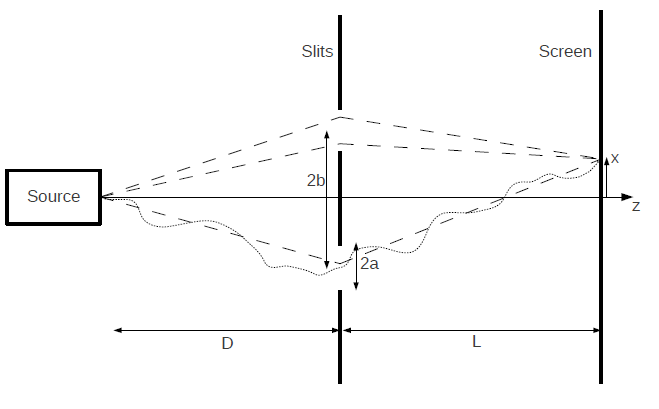
\includegraphics[width=10cm]{Imagenes/Fig8}
\caption[Esquema del experimento de la doble rendija en 2D]{Experimento de la doble rendija.}
\end{figure}
Como sabemos la probabilidad está dada por el módulo al cuadrado de la amplitud, la cual calcularemos usando el propagador. Como explicamos anteriormente hemos tomado $d=2$ en el propagador, sin embargo, vamos a explicar por qué podemos reducir aún más la complejidad del problema: consideremos la difracción por una sola rendija y que el movimiento está dividido en dos regiones, uno empezando desde la fuente y llegando a las rendijas un tiempo $T$ después de la emisión y otro de la rendija a la pantalla, este último de duración $\tau$.
\\
\\
Sin embargo, no hay nada en las leyes de la mecánica cuántica que nos diga que podemos separar el movimiento en dos tramos, esto debido a que realmente no tenemos certeza de la posición de la partícula en un tiempo $T$. En pocas palabras no sabemos cuando el electrón ha cruzado la rendija.
\\
\\
No obstante podemos considerar esta imagen clásica para estudiar el problema, veamos por qué: el electrón tiene un momentum $p_z=\hbar k_z$, el cual está relacionado con la velocidad clásica como $V_z=D/T=L/\tau$, aquí suponemos que $D$ es suficientemente grande comparado con las dimensiones en $x$ ($x,a,b\ll D,L$). Adicionalmente la longitud de onda $\lambda$ de la partícula es aproximadamente igual a la contribucion en $z$ (esto es como si tomaramos partículas que no se desvían demasiado de la trayectoria clásica). Si $\lambda \approx \lambda_z=2\pi\hbar/(mv_z)$ entonces $\lambda \ll D,L$. Esto quiere decir que el movimiento en $z$ es practicamente clásico. Note que cuánticamente es posible que el electrón pase a través de la rendija varias veces, sin embargo la probabilidad de este suceso ha de ser baja.

Teniendo en cuenta lo anterior:
\begin{eqnarray}
\nonumber K_{a,b}^{2D}((x,L+D),T+\tau;(0,0),0)&=&\int_{-\infty}^{\infty}d\omega\chi_{[b-a,b+a]}(\omega)K_{0}^{2D}((x,L+D),T+\tau;(\omega,D),T)\\
&&\nonumber \times K_{0}^{2D}((\omega,D),T;(0,0),0)\\
&=&\nonumber \frac{e^{\frac{imL^{2}}{2\hbar\tau}}}{\sqrt{2\pi i\hbar\tau/m}}\frac{e^{\frac{imD^{2}}{2\hbar T}}}{\sqrt{2\pi i\hbar T/m}}\int_{b-a}^{b+a}\frac{e^{\frac{im\omega^{2}}{2\hbar T}}}{\sqrt{2\pi i\hbar T/m}}\frac{e^{\frac{im(x-\omega)^{2}}{2\hbar\tau}}}{\sqrt{2\pi i\hbar\tau/m}}d\omega ,	
\end{eqnarray}
por tanto el propagador es el producto de dos propagadores independientes:
\begin{eqnarray}
K_z(L+D,T+\tau;0,0)&=&\frac{e^{\frac{imL^{2}}{2\hbar\tau}}}{\sqrt{2\pi i\hbar\tau/m}}\frac{e^{\frac{imD^{2}}{2\hbar T}}}{\sqrt{2\pi i\hbar T/m}}\\
K_x(x,T+\tau;0,0)&=&\int_{b-a}^{b+a}\frac{e^{\frac{im\omega^{2}}{2\hbar T}}}{\sqrt{2\pi i\hbar T/m}}\frac{e^{\frac{im(x-\omega)^{2}}{2\hbar\tau}}}{\sqrt{2\pi i\hbar\tau/m}}d\omega .
\end{eqnarray}
Una forma de comprobar que las ecuaciones (2.63) y (2.64) son correctas es ver que si quitamos las rendijas ($a\to \infty$) e integramos en $D$ en el intervalo $(-\infty,\infty)$ recuperamos el propagador de una particula libre.\\
\\
En lo que sigue nos vamos a dar a la tarea de mostrar que podemos expresar la amplitud en términos de las conocidas integrales de Fressnel, sabemos que $P(x;a,b)=|A(x;a,b)|^2$ y de (2.64):
\begin{equation}
A_1(x;a,b)=\int_{b-a}^{b+a}\frac{e^{\frac{im\omega^{2}}{2\hbar T}}}{\sqrt{2\pi i\hbar T/m}}\frac{e^{\frac{im(x-\omega)^{2}}{2\hbar\tau}}}{\sqrt{2\pi i\hbar\tau/m}}d\omega .
\end{equation} 
Organicemos de una manera diferente el exponencial de la ecuación (2.65):
\begin{eqnarray}
\nonumber \frac{m}{2\hbar\tau}(x-\omega)^{2}+\frac{m\omega^{2}}{2\hbar\tau}&=&\frac{m}{2\hbar}\left[\frac{1}{T}+\frac{1}{\tau}\right]\left[\omega^{2}-\frac{2x\omega}{\left(\frac{\tau}{T}+1\right)}+\left(\frac{x}{\frac{\tau}{T}+1}\right)^{2}-\left(\frac{x}{\frac{\tau}{T}+1}\right)^{2}\right]+\frac{mx^{2}}{2\text{\ensuremath{\hbar\tau}}}\\
&=&\nonumber \frac{m}{2\hbar}\left[\frac{1}{T}+\frac{1}{\tau}\right]\left[\omega-\frac{x}{1+\tau/T}\right]^{2}+\frac{mx^{2}}{2\text{\ensuremath{\hbar}}}\left[\frac{1}{\tau}-\frac{T}{(\tau+T)\tau}\right]\\
&=& \left[\frac{m}{2\hbar T}+\frac{m}{2\hbar\tau}\right]\left[\omega-\frac{x}{1+\tau/T}\right]^{2}+\frac{mx^{2}}{2\text{\ensuremath{\hbar}}(T+\tau)},
\end{eqnarray}
por tanto reemplazando (2.66) en (2.65)
\begin{equation}
A_{1}(x;a,b)=\frac{e^{\frac{imx^{2}}{2\hbar(T+\tau)}}}{\sqrt{2\pi i\hbar(T+\tau)/m}}\int_{b-a}^{b+a}d\omega\sqrt{\frac{T+\tau}{2\pi\hbar T\tau/m}}\ \exp\left\{ \frac{i(T+\tau)}{2\hbar T\tau/m}\left(\omega-\frac{x}{1+\tau/T}\right)^{2}\right\}
\end{equation}
Ahora si $\omega^{\prime}=\sqrt{\frac{T+\tau}{\pi\hbar T\tau/m}}\left(\omega-\frac{x}{1+\tau/T}\right)$:
\begin{equation}
\Rightarrow A_{1}(x;a,b)=\frac{e^{\frac{imx^{2}}{2\hbar(T+\tau)}}}{\sqrt{2\pi i\hbar(T+\tau)/m}}\int_{\alpha_{-}(x)}^{\alpha_{+}(x)}d\omega^{\prime}\sqrt{\frac{T+\tau}{2\pi\hbar T\tau/m}}\ \exp\left\{ \frac{i\pi\omega^{\prime 2}}{2}\right\} ,
\end{equation}
donde $\alpha_{\pm}(x)=\sqrt{\frac{T+\tau}{\pi\hbar T\tau/m}}(b\pm a)-\frac{x}{\sqrt{\pi\hbar\tau/m}}\sqrt{\frac{T}{T+\tau}}$.
Si descomponemos el exponencial de la ecuación (2.68) en su parte imaginaria y real, obtenemos las famosas integrales de Fressnel, definidas como:
\begin{equation}
C[u]\equiv \int_{0}^{u}d\omega Cos\left(\frac{\pi\omega ^2 }{2}\right)\hspace{0.3cm} ;\hspace{0.3cm} S[u]\equiv \int_{0}^{u}d\omega Sin\left(\frac{\pi\omega ^2 }{2}\right) .
\end{equation}
Así:
\begin{eqnarray}
&\nonumber A_{1}(x;a,b)=\frac{e^{\frac{imx^{2}}{2\hbar(T+\tau)}}}{\sqrt{(2i)^{2}\pi\hbar(T+\tau)/m}}\\
&\times[C[\alpha_{+}(x;a.b)]-C[\alpha_{-}(x;a.b)]+iS[\alpha_{+}(x;a.b)]-iS[\alpha_{-}(x;a.b)]]\\
&A_{2}(x;a,b)=A_{1}(x;a,-b).
\end{eqnarray}
Para dos rendijas podemos calcular la amplitud total simplemente sumando:
\begin{equation}
A(x;a,b)=A_{1}(x;a,b)+A_{2}(x;a,b).
\end{equation}


\subsection{Difracción por una rendija.}
En el caso de una sola rendija tenemos que $b=0$, además recordando que $\lambda\approx\lambda_z=h/mv_z$ ; $v_z=L/\tau=D/T$, podemos escribir:
\begin{equation}
\alpha(x,a)=\sqrt{N_F(a)}\sqrt{1+L/D}\left[	1-\frac{x}{a(1+L/D)}\right] \hspace{0.3cm};\hspace{0.3cm} N_F(a)=2a^2/\lambda L .
\end{equation}
Las integrales de Fressnel tienen un comportamiento diferente dependiendo del valor de $N_F(a)$:
\begin{eqnarray}
C(\pm u)&=&\pm\frac{1}{2}+\frac{1}{\pi u}Sin\left(\frac{\pi u^2}{2}\right),\hspace{0.3cm}u\geq 1\\
S(\pm u)&=&\pm\frac{1}{2}-\frac{1}{\pi u}Sin\left(\frac{\pi u^2}{2}\right),\hspace{0.3cm}u\geq 1 .
\end{eqnarray}
Definiendo $\eta\equiv 1+L/D$ y $\gamma=\eta-1$, en el caso $\frac{x}{a\eta}-1\gg\frac{1}{\sqrt{N_F(a)\eta}}$ encontramos que:
\begin{eqnarray}
\alpha(x,a)&\ll&-1\\
\alpha(x,-a)&\gg&1 ,
\end{eqnarray} 
por tanto:
\begin{eqnarray}
C[\alpha(x,\pm a)]&=&\pm\frac{1}{2}+\frac{1}{\pi\alpha(x,\pm a) }Sin\left(\frac{\pi \alpha(x,\pm a)^2}{2}\right)\\
S[\alpha(x,\pm a)]&=&\pm\frac{1}{2}-\frac{1}{\pi\alpha(x,\pm a) }Sin\left(\frac{\pi \alpha(x,\pm a)^2}{2}\right) .
\end{eqnarray}
Es fácil mostar que $C[\alpha_-(x,a,o)]=-C[\alpha(x,-a)]$ y $S[\alpha_-(x,a,o)]=-S[\alpha(x,-a)]$, con esto, y usando la ecuación (2.70):
\begin{eqnarray}
\nonumber & P^{\text{(1rendija)}}(x;a,b)=|A(x;a,b)|^2=\\&\frac{1}{2\lambda(L+D)}
([C(\alpha(x,a))+C(\alpha(x.-a))]^{2}+[S(\alpha(x.a))+S(\alpha(x.-a))]^{2}) .
\end{eqnarray}
Usando las ecuaciones (2.78),(2.79) y (2.80) encontramos:
\begin{equation}
P^{(\text{1rendija})}(x,a)\simeq\frac{2\gamma}{\pi^{2}\eta^{2}}\left(\frac{a^{2}}{\left(\frac{x^{2}}{\eta^{2}}-a^{2}\right)^{2}}+\frac{1}{\left(\frac{x^{2}}{\eta^{2}}-a^{2}\right)}\text{Sin}^{2}\left(\pi N_{F}(a)\frac{x}{a}\right)\right) ,
\end{equation}
en el límite $N_F(a)\ll 1\Rightarrow \frac{x}{\eta}\gg a$ ,tenemos la siguiente aproximación:
\begin{equation}
P^{(\text{1rendija})}(x,a)\simeq\frac{2\gamma}{\pi^{2}x^{2}}\text{Sin}^{2}\left(\pi N_{F}(a)\frac{x}{a}\right) .
\end{equation}
Este límite es conocido como el régimen de Fraunhofer (Pantalla lejana), Figura 2.9. Es importante recalcar que en el regimen intermedio $(N_F(a)\approx 1)$, las aproximaciones (2.81) y (2.82) siguen siendo válidas.
\begin{figure}[h]
\centering
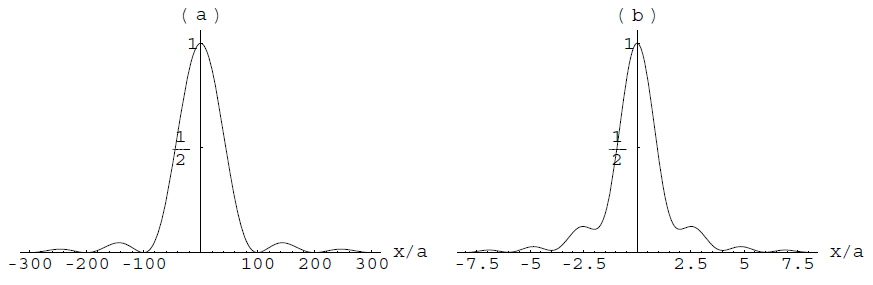
\includegraphics[width=13cm]{Imagenes/Fig9}
\caption[Patron de interferencia, 1 rendija, regimen de Fraunhofer]{Curva de difracción para una sola rendija, en la figura (a) $N_F(a)=0.01$, en (b) $N_F(a)=0.5$. Tomado de [1]}
\end{figure}
Sin embargo para $N_F(a)\ll 1$, obtenemos diferentes aproximaciones asintóticas:
\begin{eqnarray}
\nonumber &P^{(\text{1rendija})}(x)\simeq\frac{\gamma}{\eta}\left(\frac{\sqrt{N_{F}(a)}}{2a}+\frac{\text{\text{Sin}}\left(\frac{\pi}{2}N_{F}(a)\eta\left(1-\frac{x}{a\eta}\right)^{2}\right)}{2\pi\sqrt{\eta}\left(a-\frac{x}{\eta}\right)}+\frac{\text{\text{Sin}}\left(\frac{\pi}{2}N_{F}(a)\eta\left(1+\frac{x}{a\eta}\right)^{2}\right)}{2\pi\sqrt{\eta}\left(a+\frac{x}{\eta}\right)}\right)^{2}\\
&+\frac{\gamma}{\eta}\left(\frac{\sqrt{N_{F}(a)}}{2a}-\frac{\text{\text{Cos}}\left(\frac{\pi}{2}N_{F}(a)\eta\left(1-\frac{x}{a\eta}\right)^{2}\right)}{2\pi\sqrt{\eta}\left(a-\frac{x}{\eta}\right)}-\frac{\text{\text{Cos}}\left(\frac{\pi}{2}N_{F}(a)\eta\left(1+\frac{x}{a\eta}\right)^{2}\right)}{2\pi\sqrt{\eta}\left(a+\frac{x}{\eta}\right)}\right)^{2},|x|<a\eta ,
\end{eqnarray}
\begin{equation}
P^{(\text{1rendija})}(x,a)\simeq\frac{2\gamma}{\pi^{2}\eta^{2}}\left(\frac{a^{2}}{\left(\frac{x^{2}}{\eta^{2}}-a^{2}\right)^{2}}+\frac{1}{\left(\frac{x^{2}}{\eta^{2}}-a^{2}\right)}\text{Sin}^{2}\left(\pi N_{F}(a)\frac{x}{a}\right)\right), |x|>a\eta .
\end{equation}
Esto se debe a que las aproximaciones asintóticas tienen el siguiente comportamiento:
\begin{eqnarray}
&\alpha(x,\pm a)\gg 1,\hspace{0.2cm} \text{si}\hspace{0.2cm} N_F(a)\gg 1 \hspace{0.2cm} \text{y}\hspace{0.2cm} |x|<a\eta\\
&\pm\alpha(x,\mp a)\gg 1,\hspace{0.2cm} \text{si}\hspace{0.2cm} N_F(a)\gg 1 \hspace{0.2cm} \text{y}\hspace{0.2cm} |x|>a\eta .
\end{eqnarray}
La función (2.83) oscila rápidamente alrededor del valor constante $N_F(a)\gamma/2a^2\eta=1/(\lambda_z(L+D))$ en $|x|<a\eta$ y la función (2.84) decrece rapidamente a 0 en $|x|>a\eta$. La curva de difracción se muestra en la figura 2.10.
\begin{figure}[h!]
\centering
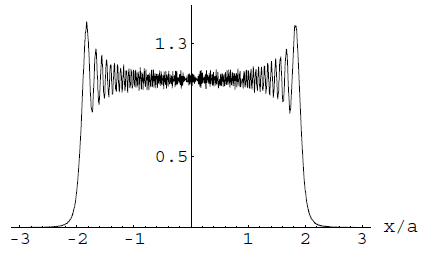
\includegraphics[width=10cm]{Imagenes/Fig10}
\caption[Patrón de interferencia, 1 rendija, regimen de Fressnel]{Curva de difracción para una sola rendija, en la figura  $N_F(a)=100$. Tomado de [1]}
\end{figure}



\subsection{Interferencia y difracción por dos rendijas.}

Podemos calcular la curva de difracción e interferencia para dos rendijas usando la siguiente expresión:
\begin{equation}
P^{(2\text{rendija})}(x;a,b)=P_{1}(x;a,b)+P_{2}(x;a,b)+I_{12}(x;a,b) ,
\end{equation}
donde:
\begin{eqnarray}
\nonumber P_{1}(x;a,b)&=&|A_1(x;a,b)|^2\\
\nonumber &=&\frac{\gamma}{2\lambda L\eta}([C(\alpha_{+}(x;a,b)-C(\alpha(x;a,b))]^{2}+[S(\alpha_{+}(x;a,b)-S(\alpha(x;a,b))]^{2})\\
P_2(x;a,b)&=&|A_2(x;a,b)|^2=P_1(x;a,-b) ,
\end{eqnarray}
y el término de interferencia:
\begin{eqnarray}
\nonumber I_{12}(x;a,b)&=& A_1(x;a,b)A_2(x;a,b)^*+A_2(x;a,b)A_1(x;a,b)^*\\
\nonumber &=&\frac{\gamma}{\lambda L\eta}([C(\alpha_{+}(x;a,b)-C(\alpha(x;a,b))][C(\alpha_{+}(x;a,-b)-C(\alpha(x;a,-b))]\\
&+& [S(\alpha_{+}(x;a,b)-S(\alpha(x;a,b))][S(\alpha_{+}(x;a,-b)-S(\alpha(x;a,-b))]) .
\end{eqnarray}
Hay que notar que en el caso de dos rendijas hay un término adicional, llamado el \textit{término de interferencia}, este es similar al encontrado en óptica. Esto resulta en un efecto de modulación de la curva de difracción dada por la suma de los términos de la ecuación (2.88).\\
\\
Definamos los números de Fressnel:
\begin{equation}
N_F(a)\equiv 2a^2/\lambda_zL ;\hspace{0.3cm} N_F(b)\equiv 2b^2/\lambda_zL ;\hspace{0.3cm} N_F\equiv 2ab/\lambda_zL=\sqrt{N_F(a)N_F(b)/2} ,
\end{equation}
en el caso de dos rendijas de ancho $2a$ y separadas por una distancia $2b$, en el caso en que $b\gg a$ tenemos los siguientes comportamientos, que se dividen en dos fases:
\begin{itemize}
\item Si $N_F\ll 1$, estamos en la \textit{fase mezclada}, es decir, encontramos una curva de interferencia modulada por la curva de difración de una rendija de tamaño $a$. En este caso estamos en el regimen de Fressnel, $N_F(a)\ll 1$. Este se muestra en la figura 2.11(a). 
\item Si $N_F\gg 1$, estamos en la \textit{fase separada}, es decir, hay dos curvas de interferencia, moduladas por las curvas de difracción correspondientes a cada rendija, cada curva centrada en $\pm b\eta$.	La forma de las curvas de difracción dependen de $N_F(a)$ y son similares al caso de una rendija (donde teniamos dos regímenes establecidos: Fressnel y Fraunhofer). En la figura 2.11(c), $N_F(a)\ll 1$ y en la figura 2.11(d) $N_F(a)\gg 1$.
\item Si $N_F\sim 1$ observamos una separación entre dos curvas de interferencia, moduladas por una curva de difracción que corresponde al de una rendija en el caso de regimen intermedio, esto se muestra en la figura 2.11(b). 
\end{itemize}
\begin{figure}[h!]
\centering
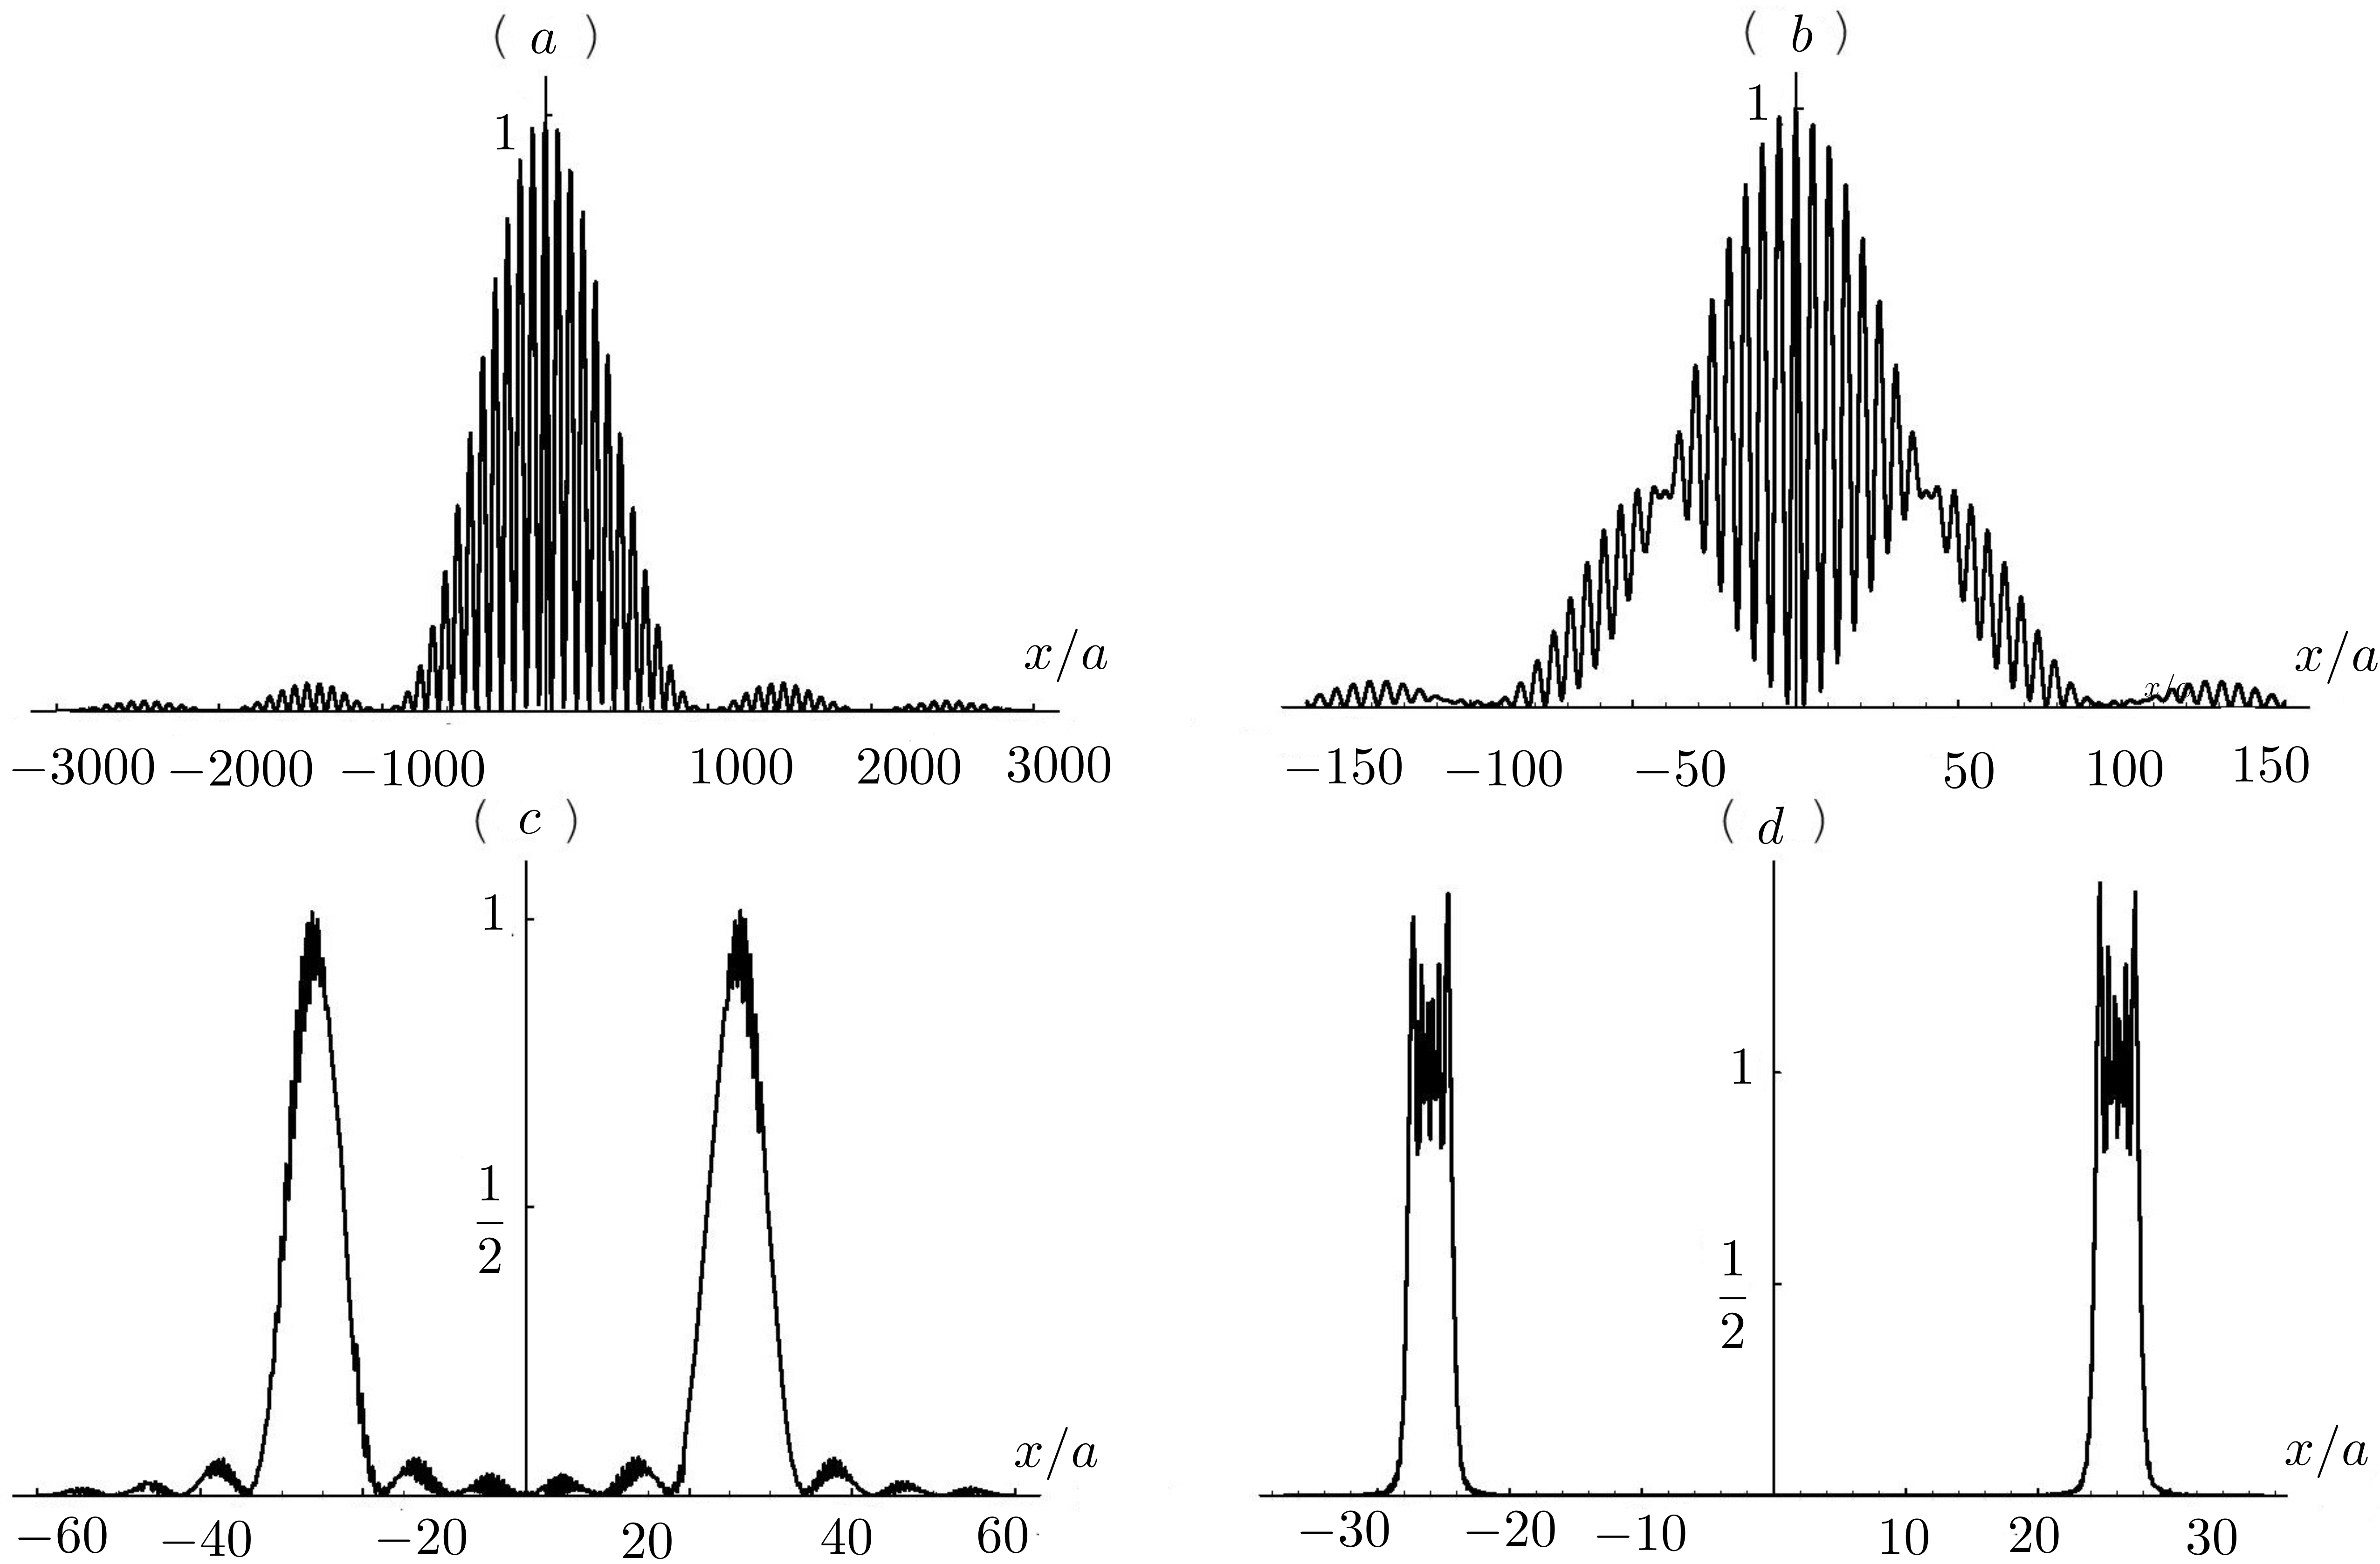
\includegraphics[width=14.5cm]{Imagenes/Fig11}
\caption[Patrón de interferencia, 2 rendijas]{Curva de difracción para dos rendijas, en la figura  $N_F(a)=0.001$ para (a), 0.015 para (b), 0.12 para (c), 6 para (d) . Tomado de [1]}
\end{figure}
\newpage
\newpage





\section{Campos escalares.}
En analogía con lo estudiado en la sección anterior para una partícula, definimos la transición vacío-vacío en presencia de una fuente $J(x)$ para un campo $\phi(x)$ como:
\begin{equation}
Z[J]=\int\mathcal{D}\phi\ \exp\left\{ i\int d^{4}x\left[\mathcal{L}(\phi)+J(x)\phi(x)+\frac{i}{2}\epsilon\phi^{2}(x)\right]\right\} .
\end{equation}
En este caso en vez de dividir el espacio-tiempo en segmentos, dividimos el espacio 4 dimensional (4D) de Minkowski en hipervolúmenes (4D) asumiendo que en cada uno de estos volúmenes $\phi(x)$ es constante. Si $\mathcal{L}=\mathcal{L}(Klein-Gordon)=\frac{1}{2}(\partial_\mu\phi\partial^\mu\phi-m^2 \phi^2)$, tenemos:
\begin{equation}
Z_{0}[J]=\text{\ensuremath{\int\mathcal{D}}}\phi\ \exp\left\{ i\int d^{4}x\left[\frac{1}{2}(\partial_{\mu}\phi\partial^{\mu}\phi-(m^{2}-i\epsilon)\phi^{2}))+J\phi\right]\right\} .
\end{equation} 	
Ahora como $\int\partial_{\mu}\phi\partial^{\mu}\phi=\int\partial_{\mu}(\phi\partial^{\mu}\phi)-\int\phi\square\phi=0-\int\phi\square\phi$, donde hemos usado que la primera integral es una cuadridivergencia y puede ser expresada como una integral de superficie, y poniendo la condición de frontera de que los campos se anulan en el borde, este término es cero. Por tanto (2.92) queda:
\begin{equation}
Z_{0}[J]=\text{\ensuremath{\int\mathcal{D}}}\phi\ \exp\left\{ -i\int d^{4}x\left[\frac{1}{2}(\phi\square\phi+(m^{2}-i\epsilon)\phi^{2}))-J\phi\right]\right\} .
\end{equation}
El campo $\phi(x)$ no satisface la ecuacion de K-G. Para evaluar $Z_0[J]$ separemos $\phi(x)$:
\begin{equation}
\phi \rightarrow \phi(x)+\phi_0(x) ,
\end{equation}
se puede probar fácilmente que $\int\phi_{0}(\square+m^{2}-i\epsilon)\phi=\int\phi(\square+m^{2}-i\epsilon)\phi_{0}$, por tanto:
\begin{eqnarray}
\nonumber \int d^{4}x\left[\frac{1}{2}\phi(\square+m^{2}-i\epsilon)\phi-J\phi\right]&\rightarrow\int d^{4}x[\frac{1}{2}\phi(\square+m^{2}-i\epsilon)\phi+\phi(\square+m^{2}-i\epsilon)\phi_{0}\\
&+\frac{1}{2}\phi_{0}(\square+m^{2}-i\epsilon)\phi_{0}-J\phi-J\phi_{0}],
\end{eqnarray}
si ahora escogemos $\phi_0$ tal que satisfaga:
\begin{equation}
(\square+m^2-i\epsilon)\phi_0(x)=J(x),
\end{equation}
entonces (2.95) queda como:
\begin{equation}
\int d^{4}x\left[\frac{1}{2}\phi(\square+m^{2}-i\epsilon)\phi-\frac{1}{2}J\phi_{0}\right].
\end{equation}
La solución a (2.96) es:
\begin{equation}
\phi_{0}(x)=-\int\triangle_{F}(x-y)J(y)d^{4}y ,
\end{equation}
donde $\triangle_F(x-y)$, llamado el propagador de Feynmann, es la función de green del operador $(\square+m^2-i\epsilon)$ y cumple:
\begin{equation}
(\square+m^2-i\epsilon)\triangle_{F}(x)=-\delta^4(x).
\end{equation}
Con todo lo anterior podemos escribir $Z_0[J]$ como:
\begin{equation}
Z_0[J]=\ \exp\left\{ -\frac{i}{2}\int d^{4}xd^{4}yJ(x)\triangle_{F}(x-y)J(y)\right\} \int\mathcal{D}\phi\ \exp\left\{ -\frac{i}{2}\int d^{4}x\left[\frac{1}{2}(\phi(\square +m^{2}-i\epsilon)\phi\right]\right\} .
\end{equation}
Por tanto hemos logrado separar el funcional generatriz en dos partes, una que depende unicamente de $J(x)$ y otra de $\phi(x)$, esta última de hecho es simplemente un número que llamaremos $\mathcal{N}$, así:
\begin{equation}
Z_{0}[J]=\mathcal{N}\ \exp\left\{ -\frac{i}{2}\int d^{4}xd^{4}yJ(x)\triangle_{F}(x-y)J(y)\right\} .
\end{equation}
\subsection{Integración funcional.}
Vamos a generalizar la fórmula de integración Gaussiana a $n$ variables discretas para luego analizar este tipo de fórmulas en el caso de cálculo funcional. Sabemos que 
\begin{equation}
\int_{-\infty}^{\infty}e^{-\frac{1}{2}ax^{2}}dx=\left(\frac{2\pi}{a}\right)^{1/2}\Rightarrow\int\ \exp\left(-\frac{1}{2}\sum a_{n}x_{n}^{2}\right)dx_{1}...dx_{n}=\frac{(2\pi)^{n/2}}{\prod_{i=1}^{n}a_{i}^{1/2}} .
\end{equation}
Sea $A$ una matriz diagonal y $x$ un vector, el producto escalar de $Ax$ y $x$ es $(x,Ax)=\sum_n a_nx_{n}^{2}$ y $det(A)=\prod_{i=1}^{n}a_i$. Por tanto podemos escribir (2.102) como:
\begin{equation}
\int\ \exp\left[-\frac{1}{2}(x,Ax)\right]d^{n}x=(2\pi)^{n/2}(detA)^{-1/2} .
\end{equation}
Si definimos la medida $dx=d^nx(2\pi)^{-n/2}$, tenemos:
\begin{equation}
\int\ \exp\left[-\frac{1}{2}(x,Ax)\right]dx=(detA)^{-1/2} ,
\end{equation}
esta ecuación puede ser extendida a formas cuadráticas $Q(x)=\frac{1}{2}(x,Ax)+(b,x)+c$. En este caso tenemos:
\begin{equation}
\int\ \exp\left[-\frac{1}{2}\left\{ (x,Ax)+(b,x)+c\right\} \right]dx=\ \exp\left[\frac{1}{2}(b,A^{-1}b)-c\right]det(A)^{-1/2} .
\end{equation}
La generalización funcional de la ecuación (2.104) es:
\begin{equation}
\int\mathcal{D}\phi\ \exp\left[-\frac{1}{2}\int\phi(x)A\phi(x)dx\right]=(detA)^{-1/2} .
\end{equation}
Así si partimos de $Z_{0}[J]=\int\mathcal{D}\phi\ \exp\left\{ -i\int\left[\frac{1}{2}\phi(\square+m^{2}-i\epsilon)\phi-J\phi\right]d^{4}x\right\} $ y aplicando (2.105) y (2.106) con $A=i(\square+m^2-i\epsilon)$, $b=-iJ(x)$ y $c=0$. Tenemos:
\begin{equation}
Z_{0}[J]=\ \exp\left[\frac{i}{2}\int J(x)(\square+m^{2}-i\epsilon)^{-1}J(y)dxdy\right]det(i(\square+m^{2}-i\epsilon))^{-1/2} .
\end{equation}
Como sabemos  de (2.99) $(\square +m^2-i\epsilon)^{-1}=-\triangle_F(x-y)$ y con la ecuación (2.106):
\begin{equation}
Z_0[J]=\ \exp\left\{ -\frac{i}{2}\int d^{4}xd^{4}yJ(x)\triangle_{F}(x-y)J(y)\right\} \int\mathcal{D}\phi\ \exp\left\{ -\frac{i}{2}\int d^{4}x\left[\frac{1}{2}(\phi(\square +m^{2}-i\epsilon)\phi\right]\right\} . 
\end{equation}
Esta es la misma ecuación que (2.100)!

\subsection{Funciones de Green de la partícula libre.}
Si expandimos la amplitud de transición en serie:
\begin{equation}
Z_{0}[J]=\mathcal{N}\left\{ 1-\frac{i}{2}\int dxdyJ(x)\triangle_{F}(x-y)J(y)+\frac{1}{2!}\left(\frac{i}{2}\right)^{2}\left[\int d^{4}xd^{4}yJ(x)\triangle_{F}(x-y)J(y)\right]^{2}+...\right\},
\end{equation}
e introduciendo la transformada de Fourier de $J(x)$, 
\begin{equation}
J(x)=\int J(p)e^{-ip\cdot x}d^4p,
\end{equation}
teniendo en cuenta que para abreviar hemos escrito los diferenciales en el cuadrivolumen como $d^4h\equiv dh$, tenemos:
\begin{eqnarray}
\nonumber -\frac{i}{2}\int J(x)\triangle_F(x-y)J(y)dxdy&=&-\frac{i}{2(2\pi)^{4}}\int\frac{J(p_{1})e^{-ip_{1}\cdot x}J(p_{2})e^{-ip_{2}\cdot y}e^{-ik(x-y)}dxdydkdp_{1}dp_{2}}{k^{2}-m^{2}+i\epsilon}\\
\nonumber &=& -\frac{i}{2(2\pi)^{4}}\int\frac{J(p_{1})J(p_{2})e^{-ix(p_{1+k})}e^{-iy(p_{2}-k)}dxdydkdp_{1}dp_{2}}{k^{2}-m^{2}+i\epsilon}.\\
\nonumber \text{Integrando en x,y} &&\\
\nonumber &=& -\frac{i(2\pi)^{8}}{2(2\pi)^{4}}\int\frac{J(p_{1})J(p_{2})\delta(p_{1}+k)\delta(p_{2}-k)dkdp_{1}dp_{2}}{k^{2}-m^{2}+i\epsilon}\\
&=& -\frac{i(2\pi)^{4}}{2}\int\frac{J(k)J(-k)d^{4}k}{k^{2}-m^{2}+i\epsilon}.
\end{eqnarray}
Si identificamos la expresión anterior mediante las reglas de la figura 2.12,
\begin{SCfigure}[1][h]
\caption[Diagrama de Feynmann segunda cuantización]{Diagrama de Feynmann segunda cuantización}
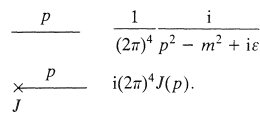
\includegraphics[width=5.5cm]{Imagenes/Fig12}
\end{SCfigure}
entonces la integral (2.111) puede ser identificada con el diagrama que aparece en la figura 2.13:
\begin{SCfigure}[1][h!]
\caption[Diagrama de Feynmann segunda cuantización]{Representación de (2.111)}
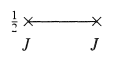
\includegraphics[width=3cm]{Imagenes/Fig13}
\end{SCfigure}
\\
\\
\\
por tanto finalmente:
\begin{equation}
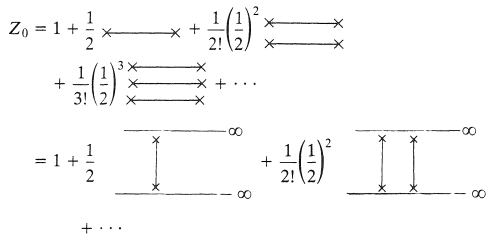
\includegraphics[width=12cm]{Imagenes/Fig14}
\end{equation}
Podemos interpretar esta serie como la propagación y posterior aniquilación de  una partícula entre fuentes, de dos partículas entre fuentes y así sucesivamente. Tenemos por tanto una teoría de muchos cuerpos, lo cual es consistente con nuestra idea inicial de utilizar un campo. Cada término en la serie es una función de Green por tanto $Z_0[J]$ es llamada un \textit{funcional generatriz} para las funciones de Green de la teoría.
\\
\\
Para entender esto analicemos la expansión en series de un funcional, primero recordemos la expansion en series de una funcion de $k$ variables $F(y_1,...,y_k)$:
\begin{equation}
F\{y\}=F(y_{1},..,y_{k})=\sum_{n=0}^{\infty}\sum_{i_{1}}^{k}...\sum_{i_{n}}^{k}\frac{1}{n!}T_{n}(i_{1},...,i_{n})y_{i_{1}}...y_{i_{n}},
\end{equation}
donde
\begin{equation}
T_{n}(i_{1},...,i_{n})=\frac{\partial F\{y\}}{\partial y_{1}...\partial y_{n}}|_{y=0} .
\end{equation}
Si vamos al caso de muchas variables continuas $i\rightarrow x_1, y_i\rightarrow y(x),\sum_i\rightarrow \int dx$, entonces obtenemos la serie de potencias de un funcional:
\begin{equation}
F[y]=\sum_{n=0}^{\infty}\int dx_{1}...dx_{n}\frac{1}{n!}T_{n}(x_{1},...,x_{n})y(x_{1})...y(x_{n}),
\end{equation}
y en este caso:
\begin{equation}
T_{n}(x_{1},...,x_{n})=\frac{\delta}{\delta y(x_{1})}...\frac{\delta}{\delta y(x_{n})}F[y]|_{y=0} .
\end{equation}
$F[y]$ es llamado el \textit{funcional generatriz} de las funciones  $T_{n}(x_{1},...,x_{n})$. Si escogemos una normalización tal que $Z_0[J]|_{J=0}=1 \Rightarrow \mathcal{N}=1$, por tanto:
\begin{equation}
Z_{0}[J]=\ \exp\left\{ -\frac{i}{2}\int dxdyJ(x)\triangle_{F}(x-y)J(y)\right\} .
\end{equation}
Asi $Z_0[J]$ es el funcional generatriz de:
\begin{equation}
\tau(x_{1},...,x_{n})=\frac{1}{i^{n}}\frac{\delta^{n}Z_{o}[J]}{\delta J(x_{1})...\delta J(x_{n})}|_{J=0}.
\end{equation}
En analogía con la ecuación (2.56) tenemos:
\begin{equation}
\frac{\delta^{n}Z_{o}[J]}{\delta J(x_{1})...\delta J(x_{n})}|_{J=0}=i^{n}\langle0|T[\phi(x_{1})...\phi(x_{n})]|0\rangle ,
\end{equation}
entonces:
\begin{equation}
\tau(x_1,...,x_n)=\langle0|T[\phi(x_{1})...\phi(x_{n})]|0\rangle .
\end{equation}
A las funciones $\tau(x_1,...,x_n)$ se les llama funciones de Green o funciones de n-puntos, calculemos algunas, empecemos con la función de 2-puntos:
\begin{equation}
\tau(x,y)=-\frac{\delta^2Z_0[J]}{\delta J(x)\delta J(y)}|_{J=0} ,
\end{equation}
\begin{eqnarray}
\nonumber \Rightarrow \frac{1}{i}\frac{\delta Z_{0}[J]}{\delta J(x)}&=&-\int\triangle_{F}(x-x_{1})J(x_{1})\times\ \exp\left\{ -\frac{i}{2}\int dxdy\text{\ensuremath{\triangle}}_{F}(x_{1}-x_{2})J(x_{1})J(x_{2})\right\}\\
\nonumber &=& -\int\triangle_{F}(x-x_{1})J(x_{1})\text{\ensuremath{\times}Exp}\left\{ \frac{-i}{2}\int J\triangle_{F}J\right\} ,\\ 
\nonumber \Rightarrow \frac{1}{i}\frac{\delta}{\delta J(y)}\frac{1}{i}\frac{\delta Z_{0}[J]}{\delta J(x)}&=&\int\triangle_{F}(x-x_{1})J(x_{1})\int\triangle_{F}(y-x_{1})J(x_{1})\text{\ensuremath{\times}Exp}\left\{ \frac{-i}{2}\int J\triangle_{F}J\right\}\\
&&+ i\triangle_{F}(x-y)\text{\ensuremath{\times}Exp}\left\{ \frac{-i}{2}\int J\triangle_{F}J\right\} ,
\end{eqnarray}
evaluando en $J=0$ la expresión (2.122) tenemos:
\begin{equation}
\tau(x,y)=i\triangle_F(x-y) .
\end{equation}
Pero, ¿cuál es el significado físico de esta expresión? Sabemos que:
\begin{equation}
\tau(x,y)=\langle0|T[\phi(x)\phi(y)]|0\rangle=\Theta(x_{0}-y_{0})\langle0|\phi(x)\phi(y)|0\rangle+\Theta(y_{0}-x_{0})\langle0|\phi(y)\phi(x)|0\rangle ,
\end{equation}          
si descomponemos el campo $\phi(x)$ como:
\begin{eqnarray}
\phi^{(+)}(x)&=&\int\frac{d^{3}k}{[(2\pi)^{3}2\omega_{k}]^{1/2}}f_{k}(x)a(k)\\
\phi^{(-)}(x)&=&\int\frac{d^{3}k}{[(2\pi)^{3}2\omega_{k}]^{1/2}}f_{k}^*(x)a^\dagger(k),
\end{eqnarray}
y reemplazamos en (2.125), la expresión que sobrevive es:
\begin{equation}
\tau(x,y)=\Theta(x_{0}-y_{0})\langle0|\phi^{(+)}(x)\phi^{(-)}(y)|0\rangle+\Theta(y_{0}-x_{0})\langle0|\phi^{(+)}(y)\phi^{(-)}(x)|0\rangle .
\end{equation}
Estas son las amplitudes para un partícula que es creada en el evento $(y_0,y)$, se propaga y es posteriormente destruida en $(x_0,x)$ o una partícula que es creada en el evento $(x_0,x)$, se propaga y es posteriormente destruida en $(y_o,y)$. Lo anterior se ve representado en la figura 2.14.
\begin{figure}[h!]
\centering
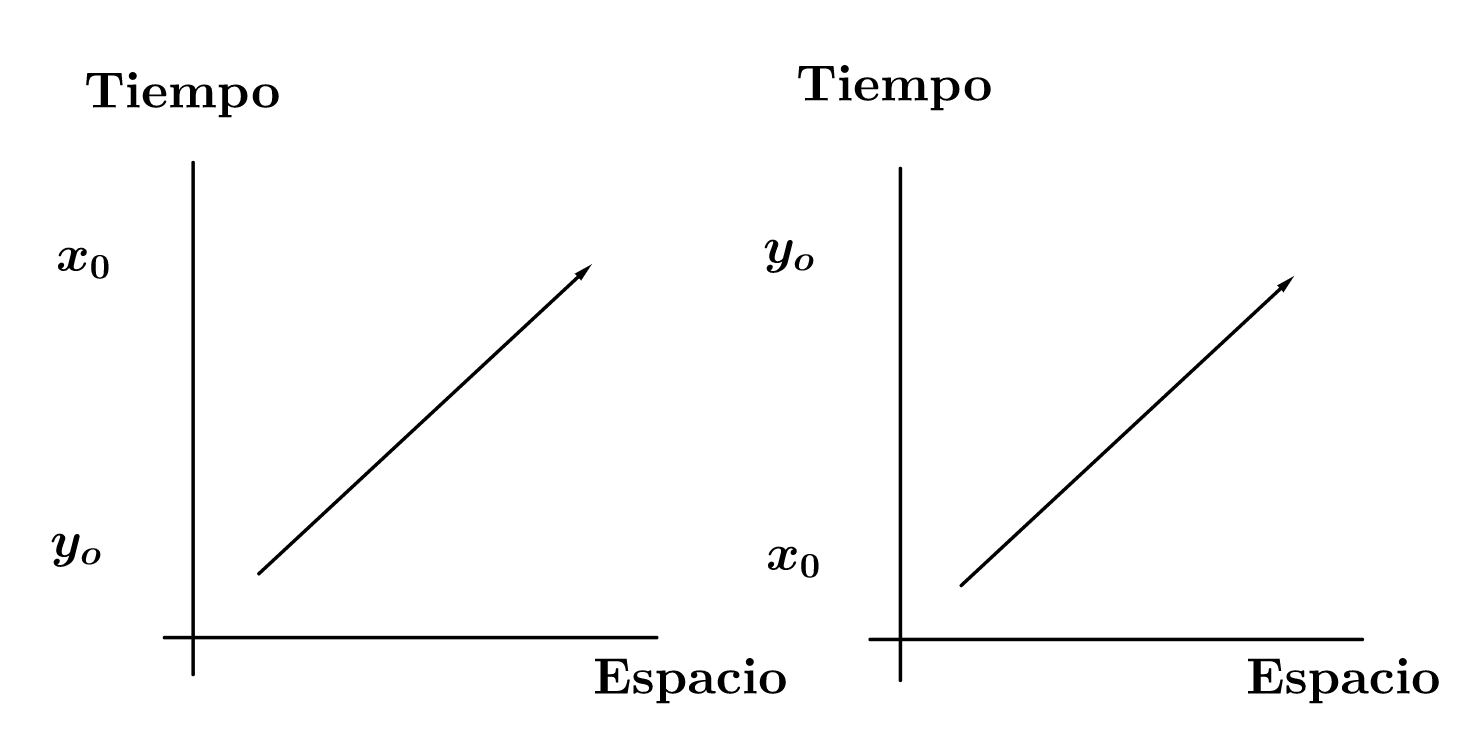
\includegraphics[width=11cm]{Imagenes/Fig15}
\caption[Representación gráfica de la función de 2-puntos ]{Representación gráfica de la ecuación 2.127}
\end{figure}
\\
\\
Es claro ahora que la función de 1-punto es:
\begin{equation}
\tau(x)=\langle 0|\phi(x)|0\rangle=0 .
\end{equation}
Calculemos entonces la función de 3-puntos, partiendo de (2.122):
\begin{eqnarray}
\nonumber\left(\frac{1}{i}\right)^{3}\frac{\delta}{\delta J_{1}}\frac{\delta}{\delta J_{2}}\frac{\delta}{\delta J_{3}}Z_{0}[J]&=&-i\triangle_{F}(x_{3}-x_{2})\int\triangle_{F}(x_{1}-x)J(x)dx\ \exp\left\{ \frac{-i}{2}\int J\triangle_{F}J\right\}\\
\nonumber && -i\triangle_{F}(x_{2}-x_{1})\int\triangle_{F}(x_{3}-x)J(x)dx\ \exp\left\{ \frac{-i}{2}\int J\triangle_{F}J\right\}\\
\nonumber &&-i\triangle_{F}(x_{3}-x_{1})\int\triangle_{F}(x_{2}-x)J(x)dx\ \exp\left\{ \frac{-i}{2}\int J\triangle_{F}J\right\}\\
\nonumber &&-\int\triangle_{F}(x_{3}-x)J(x)dx\int\triangle_{F}(x_{2}-x)J(x)dx\\
&&\times\int\triangle_{F}(x_{1}-x)J(x)dx\ \exp\left\{ \frac{-i}{2}\int J\triangle_{F}J\right\} ,
\end{eqnarray}
si evaluamos en $J=0$ la ecuación (2.129) vemos que $\tau(x_1,x_2,x_3)=0$. Para encontrar la función de 4-puntos derivamos de nuevo, los términos que sobreviven al hacer $J=0$ son:
\begin{eqnarray}
\nonumber \tau(x_1,x_2,x_3,x_4)&=&\langle 0|T[\phi(x_1)\phi(x_2)\phi(x_3)\phi(x_4)]|0\rangle\\
\nonumber &&-[\triangle_{F}(x_{3}-x_{2})\triangle_{F}(x_{1}-x_{4})\\
\nonumber &&+\triangle_{F}(x_{2}-x_{1})\triangle_{F}(x_{3}-x_{4})\\
&&+\triangle_{F}(x_{3}-x_{1})\triangle_{F}(x_{2}-x_{4})].
\end{eqnarray}
La ecuación (2.130) es el producto de funciones de 2-puntos:
\begin{equation}
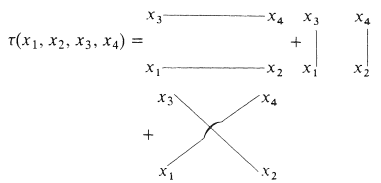
\includegraphics[width=8cm]{Imagenes/Fig16}.
\end{equation}
Así uno puede darse cuenta que si $n$ es impar la función de n-puntos se anula y si es par, es la suma de los productos de las diferentes permutaciones de funciones de 2-puntos.


\subsection{Funcional generatriz para campos interactuantes.}
Ahora debemos lidiar con el problema de encontrar el funcional generatriz para el caso de una teoría con términos de interacción en $\mathcal{L}$, en general para campos escalares $\mathcal{L}=\frac{1}{2}\left[\partial_{\mu}\phi\partial^{\mu}\phi-m^{2}\phi^{2}\right]+\mathcal{L}_{int}$. El funcional generatriz normalizado, con $S=\int \mathcal{L}dx$ es:
\begin{equation}
\frac{\int\mathcal{D}\phi\ \exp\left(iS+\int J\phi dx\right)}{\int\mathcal{D}\phi\ \exp\left(iS\right)} .
\end{equation}
Por tanto queremos encontrar la ecuación diferencial que obedece $Z[J]$ y resolverla en términos de $Z_0[J]$. Para esto primero veamos la ecuación diferencial que satiscace $Z_0[J]$. Sabemos que:
\begin{equation}
\frac{1}{i}\frac{\delta Z_{0}[J]}{\delta J(x)}=-\int\triangle_{F}(x-y)J(y)dy\ \exp\left\{ \frac{-i}{2}\int J\triangle_{F}Jdxdy\right\} ,
\end{equation}
por tanto, si aplicamos$(\square +m^2)$ a izquierda y derecha de (2.133), tenemos:
\begin{equation}
(\square +m^{2})\frac{1}{i}\frac{\delta Z_{0}[J]}{\delta J(x)}=J(x)Z_{0}[J] .
\end{equation}
Esta es la ecuación diferencial que buscabamos, si definimos el funcional $\hat{Z}_0[\phi]=\frac{e^{iS}}{\int \mathcal{D}\phi e^{iS}}$, notamos que:

\begin{equation}
Z[J]=\int\mathcal{D}\phi\hat{Z}[\phi]\ \exp\left\{ i\int J\phi dx\right\} .
\end{equation}
Esta última ecuación define el análogo funcional a la transformada de Fourier, si hacemos la derivada funcional de $\hat{Z}_0[\phi]$ obtenemos:
\begin{equation}
i\frac{\delta\hat{Z}[\phi]}{\delta\phi}=\left\{ (\square+m^{2})\phi-\frac{\partial\mathcal{L}_{int}}{\partial\phi}\right\} \hat{Z}[\phi] .
\end{equation}
Si en el lado derecho de la ecuacion (2.135) multiplicamos por $\ \exp[i\int J\phi dx]$, integramos en $\phi(x)$ y cambiamos $\phi \rightarrow \frac{1}{i}\frac{\delta}{\delta J}$, conseguimos la siguiente ecuación:
\begin{equation}
RHS(1.135)=\left\{ (\square +m^{2})\frac{1}{i}\frac{\delta}{\delta J}-\mathcal{L}_{int}^{\prime}\left[\frac{1}{i}\frac{\delta}{\delta J}\right]\right\} Z[J],
\end{equation} 
si hacemos lo mismo en el lado izquierdo nos queda:
\begin{eqnarray}
\nonumber LHS(2.135)=i\int\mathcal{D}\phi\frac{\delta\hat{Z}[\phi]}{\delta\phi}\ \exp\left(i\int J\phi dx\right)&=& i\hat{Z}[\phi]\ \exp\left(i\int J\phi dx\right)\\
\nonumber &&+\int\mathcal{D}\phi J(x)\hat{Z}[\phi]\ \exp\left(i\int J\phi dx\right).\\
\end{eqnarray}
El primer término del lado derecho de la ecuación (2.138) es un término de superficie, por tanto se anula. Entonces, la ecuación que cumple $Z[J]$ es:
\begin{equation}
\left\{ (\square+m^{2})\frac{1}{i}\frac{\delta}{\delta J}-\mathcal{L}_{int}^{\prime}\left[\frac{1}{i}\frac{\delta}{\delta J}\right]\right\} Z[J]=J(x)Z[J].
\end{equation}
Vamos a probar que la solución de esta ecuación es:
\begin{equation}
Z[J]=\mathcal{N}\ \exp\left[i\int\mathcal{L}_{int}\left(\frac{1}{i}\frac{\delta}{\delta J(x)}\right)dx\right]Z_{0}[J],
\end{equation} 
para esto probemos primero la siguiente identidad:
\begin{equation}
\ \exp\left[-i\int\mathcal{L}_{int}\left(\frac{1}{i}\frac{\delta}{\delta J(y)}\right)dy\right]J(x)\ \exp\left[i\int\mathcal{L}_{int}\left(\frac{1}{i}\frac{\delta}{\delta J(y)}\right)dy\right]=J(x)-\mathcal{L}_{int}^{\prime}\left[\frac{1}{i}\frac{\delta}{\delta J(x)}\right] .
\end{equation}
Sabemos que el conmutador $\left[J(x),\frac{1}{i}\frac{\delta}{\delta J(y)}\right]=i\delta(x-y)\Rightarrow\left[J(x),\frac{1}{i}\frac{\delta^{n}}{\delta J^{n}(y)}\right]=i\delta(x-y)n\left(\frac{1}{i}\frac{\delta}{\delta J(y)}\right)^{n-1}$, con esto podemos calcular:
\begin{eqnarray}
\nonumber \left[J(x),\int F\left(\frac{1}{i}\frac{\delta}{\delta J(y)}\right)dy\right]&=&\left[J(x),\int\left\{ F[0]+\frac{1}{i}\frac{\delta}{\delta J(y)}F^{\prime}[0]+...+\left(\frac{1}{i}\frac{\delta}{\delta J(y)}\right)^{n}\frac{F^{n}[0]}{n!}\right\} dy\right]\\
\nonumber &=& \left[J(x),\int\sum_{n=0}^{\infty}\frac{1}{n!}\left(\frac{1}{i}\frac{\delta}{\delta J(y)}\right)^{n}F^{n}[0]\right]\\
\nonumber &=& \sum_{n=0}^{\infty}\frac{1}{n!}\int i\delta(x-y)n\left(\frac{1}{i}\frac{\delta}{\delta J(y)}\right)^{n-1}F^{n}[0]dy\\
&=& i\sum_{k=1}^{\infty}\frac{1}{k!}\left(\frac{1}{i}\frac{\delta}{\delta J(y)}\right)^{k}F^{k+1}[0]=iF^{\prime}\left(\frac{1}{i}\frac{\delta}{\delta J(y)}\right) .
\end{eqnarray}
De la fórmula de Hausdorff tenemos que:
\begin{equation}
e^ABe^{-A}=B+[B,A]+\frac{1}{2!}[A,[A,B]]+...
\end{equation}
y si $A=-i\int\mathcal{L}_{int}\left(\frac{1}{i}\frac{\delta}{\delta J(y)}\right)dy$ y $B=J(x)$, tenemos que sólo los dos primeros términos de la ecuación (2.143) contribuyen y usando el resultado de (2.142) obtenemos:
\begin{equation}
\ \exp\left[-i\int\mathcal{L}_{int}\left(\frac{1}{i}\frac{\delta}{\delta J(y)}\right)dy\right]J(x)\ \exp\left[i\int\mathcal{L}_{int}\left(\frac{1}{i}\frac{\delta}{\delta J(y)}\right)dy\right]=J(x)-\mathcal{L}_{int}^{\prime}\left[\frac{1}{i}\frac{\delta}{\delta J(x)}\right].
\end{equation}
Ahora veamos lo siguiente:
\begin{equation}
J(x)Z[J]=\mathcal{N}J(x)\ \exp\left[i\int\mathcal{L}_{int}\left(\frac{1}{i}\frac{\delta}{\delta J(x)}\right)dx\right]Z_{0}[J],
\end{equation}
si hacemos el siguiente truco para introducir:
\begin{equation}
1=\ \exp\left[i\int\mathcal{L}_{int}\left(\frac{1}{i}\frac{\delta}{\delta J(x)}\right)dx\right]\times\ \exp\left[-i\int\mathcal{L}_{int}\left(\frac{1}{i}\frac{\delta}{\delta J(x)}\right)dx\right],
\end{equation}
\begin{eqnarray}
\nonumber \Rightarrow J(x)Z[J]&=&\mathcal{N}\ \exp\left[i\int\mathcal{L}_{int}\left(\frac{1}{i}\frac{\delta}{\delta J(x)}\right)dx\right]\times\left[J(x)-\mathcal{L}_{int}^{\prime}\left[\frac{1}{i}\frac{\delta}{\delta J(x)}\right]\right]Z_{0}[J]\\
\nonumber &=&\mathcal{N}\ \exp\left[i\int\mathcal{L}_{int}\left(\frac{1}{i}\frac{\delta}{\delta J(x)}\right)dx\right](\square+m^{2})\frac{1}{i}\frac{\delta Z_{0}[J]}{\delta J(x)}\\
&&-\mathcal{N}\ \exp\left[i\int\mathcal{L}_{int}\left(\frac{1}{i}\frac{\delta}{\delta J(x)}\right)dx\right]\mathcal{L}_{int}^{\prime}\left[\frac{1}{i}\frac{\delta}{\delta J(x)}\right]Z_{0}[J].
\end{eqnarray}
Así:
\begin{equation}
\left\{ (\square+m^{2})\frac{1}{i}\frac{\delta}{\delta J}-\mathcal{L}_{int}^{\prime}\left[\frac{1}{i}\frac{\delta}{\delta J}\right]\right\} Z[J]=J(x)Z[J].
\end{equation}
Esta es la ecuación diferencial que teníamos al principio (2.139), por tanto la propuesta (2.140) es correcta.
\newpage


\section{Campos fermiónicos.}
En la aproximación de cuantización canónica el campo $\psi(x)$ es tratado como un operador que obedece relaciones de anticonmutación a tiempos iguales, ${\psi(x),\bar{\psi}(y)}|_{x_0=y_0}=i\delta (x-y)$. Por otro lado en la aproximación funcional, el funcional generatriz es una integral funcional sobre los campos, para el caso de campos escalares estos son tratados como funciones que llevan números complejos a números complejos y conmutan. En el caso de campos fermiónicos es necesario que los campos sean funciones de números complejos anticonmutantes, estos números se conocen como \textit{variables de Grassmann}.
\\
\\
Los generadores $C_i$ de un álgebra de Grassmann n-dimensional cumplen la relación:
\begin{equation}
{C_i,C_j}=0\Rightarrow C_i^2=0 .
\end{equation}
En el caso 1-D la expansión en series de una función solo tiene dos términos, $f(c)=a+bC$. La diferenciación es de dos tipos, izquierda y derecha:
\begin{equation}
\frac{\partial^{L}}{\partial C_{i}}(C_{1}C_{2})=\delta_{i1}C_{2}-\delta_{i2}C_{1};\hspace{0.3cm}\frac{\partial^{R}}{\partial C_{i}}(C_{1}C_{2})=C_{1}\delta_{i2}-C_{2}\delta_{i1},
\end{equation}
también tenemos que:
\begin{eqnarray}
\nonumber \left\{ \frac{\partial}{\partial C_{i}},C_{j}\right\} C&=&\frac{\partial}{\partial C_{i}}(C_{j}C)+C_{j}\frac{\partial C}{\partial C_{i}}=\delta_{ij}C\\
\Rightarrow \left\{ \frac{\partial}{\partial C_{i}},C_{j}\right\} &=& \delta_{ij}.
\end{eqnarray} 
De la relación (2.151) se desprende que en el caso 1-D, $\left\{ \frac{d}{dC},C\right\} =1$. También se tiene que:
\begin{equation}
\left\{ \frac{\partial}{\partial C_{i}},\frac{\partial}{\partial C_{j}}\right\} =0\Rightarrow\frac{\partial^{2}}{\partial C_{i}^{2}}=0 .
\end{equation}
La ecuación (2.152) implica que no hay una operacion inversa a la diferenciación, por tanto debemos definir la integración de una manera razonable. Esto se consigue al pedir que la integración sea invariante bajo translaciones de la variable independiente, es decir que se cumpla:
\begin{equation}
\int_{-\infty}^{\infty}dxf(x)=\int_{-\infty}^{\infty}dxf(x+c) .
\end{equation}
De este requerimiento se concluye que debemos tener:
\begin{eqnarray}
\int dC=&0&; \hspace{0.3 cm} \int CdC=1,\\
\nonumber \text{en el caso n-dimensional}&&\\
\int dC_i=&0&; \hspace{0.3 cm} \int C_idC_i=1 ,
\end{eqnarray}
por tanto la integración y la derivación son la misma operación. Exploremos ahora el comportamiento de las integrales gaussianas en variables de Grassmann. Sean $\eta,\bar{\eta}$ variables de Grassmann, tenemos:
\begin{eqnarray}
e^{-\bar{\eta}\eta}&=&1-\bar{\eta}\eta\\
\Rightarrow\int d\bar{\eta}d\eta e^{-\bar{\eta}\eta}&=&\int d\bar{\eta}d\eta-\int d\bar{\eta}d\eta\bar{\eta}\eta=\int d\bar{\eta}d\eta\bar{\eta\eta}=1,
\end{eqnarray}
ahora hagamos una generalización a más dimensiones, sea $\text{\ensuremath{\bar{\eta}}=\ensuremath{\left(\begin{array}{c}
\bar{\eta_{1}}\\
\bar{\eta_{2}}
\end{array}\right)}}$;$\text{\ensuremath{\eta}=\ensuremath{\left(\begin{array}{c}
\eta_{1}\\
\eta_{2}
\end{array}\right)}}$, entonces:
\begin{equation}
\bar{\eta}^T\eta\equiv \bar{\eta}\eta=\bar{\eta}_1\eta_1+\bar{\eta}_2\eta_2\Rightarrow (\bar{\eta}\eta)^2=2\bar{\eta}_1\eta_1\bar{\eta}_2\eta_2\Rightarrow (\bar{\eta}\eta)^{3+n}=0 \;n=0,1,... 
\end{equation}
De la ecuación (2.158) podemos concluir que:
\begin{equation}
e^{-\bar{\eta}\eta}=1-(\bar{\eta}_1\eta_1+\bar{\eta}_2\eta_2)+\bar{\eta}_1\eta_1\bar{\eta}_2\eta_2\Rightarrow \int d\bar{\eta}d\eta e^{-\bar{\eta}\eta}=1.
\end{equation}
Ahora si hacemos el cambio de variables $\eta=M\alpha$ y $\bar{\eta}=N\bar{\alpha}$, donde $(M,N)$ son matrices $2\times 2$ y $(\bar{\alpha},\alpha)$ son las nuevas variables de Grassman independientes tenemos:
\begin{equation}
\eta_{1}\eta_{2}=(M_{11}\alpha_{1}+M_{12}\alpha_{2})(M_{21}\alpha_{1}+M_{22}\alpha_{2})=(M_{11}M_{22}-M_{12}M_{21})\alpha_{1}\alpha_{2}=det(M)\alpha_{1}\alpha_{2},
\end{equation}
para preservar la integración se debe mantener la condición:
\begin{equation}
\int d\eta_{1}d\eta_{2}\eta_{1}\eta_{2}=\int d\alpha_{1}d\alpha_{2}\alpha_{1}\alpha_{2}\Rightarrow d\eta_{1}d\eta_{2}=(detM)^{-1}d\alpha_{1}d\alpha_{2}.
\end{equation}
Sustituyendo (2.160) en (2.159):
\begin{eqnarray}
\nonumber (det(MN))^{-1}\int d\bar{\alpha}d\alpha e^{-\bar{\alpha}M^{T}N\alpha}=1,&\text{pero como,}& \left[det(MN)\right]^{-1}=\left[det(M^{T}N)\right]^{-1},\\
\nonumber &\text{si}\ A=M^TN&\Rightarrow \int d\bar{\alpha}d\alpha e^{-\bar{\alpha}A\alpha}=det(A).\\
\end{eqnarray}
Para describir un campo, en el caso que nos interesa, (el campo de Dirac) debemos pasar a un álgebra infinito-dimensional, por tanto:
\begin{equation}
\{C(x),C(y)\}=0; \ \frac{\partial^{LR}C(x)}{\partial C(y)}=\delta(x-y); \ \int dC(x)=0; \ \int dC(x)C(x)=1.
\end{equation}
En analogía con la ecuación (2.91) construimos el funcional generatriz para el campo de Dirac usando en este caso $\mathcal{L}_D=i\bar{\psi}\gamma^{\mu}\partial_{\mu}\psi-m\bar{\psi}\psi$, así tenemos:
\begin{equation}
Z_{0}[\eta,\bar{\eta}]=\frac{1}{\mathcal{N}}\int\mathcal{D}\bar{\psi}\mathcal{\mathcal{D}}\psi\ \exp\left\{ i\int\left[\bar{\psi}\gamma^{\mu}\partial_{\mu}\psi-m\bar{\psi}\psi+\bar{\eta}\psi+\bar{\psi}\eta\right]dx\right\} ,
\end{equation}
donde escogemos la normalización tal que:
\begin{equation}
Z_{0}[0,0]=1\Rightarrow\mathcal{N}=\int\mathcal{D}\bar{\psi}\mathcal{\mathcal{D}}\psi\ \exp\left\{ i\int\left[\bar{\psi}\gamma^{\mu}\partial_{\mu}\psi-m\bar{\psi}\psi\right]dx\right\} .
\end{equation}
En este caso $\bar{\eta}$ es la fuente de $\bar{\psi}$ y $\eta$ es la fuente de $\psi$. Con el objetivo de simplificar la notación definamos $S^{-1}\equiv i\gamma^{\mu}\partial_{\mu}-m$, entonces:
\begin{equation}
Z_{0}[\eta,\bar{\eta}]=\frac{1}{\mathcal{N}}\int\mathcal{D}\bar{\psi}\mathcal{\mathcal{D}}\psi\ \exp\left\{ i\int\left[\bar{\psi}S^{-1}\psi+\bar{\eta}\psi+\bar{\psi}\eta\right]dx\right\}.
\end{equation} 
Si $Q(\psi,\bar{\psi})=\bar{\psi}S^{-1}\psi+\bar{\eta}\psi+\bar{\psi}\eta$, los valores de $\bar{\psi},\psi$ que minimizan Q son $\psi_m=-S\eta$ y $\bar{\psi}_m=-\bar{\eta}S$, por tanto $Q_m=-\bar{\eta}S\eta$. Así $Q=Q_m+(\bar{\psi}-\bar{\psi}_m)S^{-1}(\psi-\psi_m)$. Con lo anterior podemos escribir la ecuación (2.166) como:
\begin{equation}
Z_{0}[\eta,\bar{\eta}]=\frac{1}{\mathcal{N}}\int\mathcal{D}\bar{\psi}\mathcal{\mathcal{D}}\psi\ \exp\left\{ i\int\left[Q_{m}+(\bar{\psi}-\bar{\psi}_{m})S^{-1}(\psi-\psi_{m})\right]dx\right\} .
\end{equation}
Ahora, solo dos terminos del exponencial en (2.167) sobreviven: el que tiene que ver con $Q_m$ ya que este es independiente de $(\psi,\bar{\psi})$ y:
\begin{equation}
\int\mathcal{D}\bar{\psi}\mathcal{\mathcal{D}}\psi\ \exp\left\{ i\int\left[(\bar{\psi}S^{-1}\psi\right]dx\right\} =det(iS^{-1}) .
\end{equation}
Con lo anterior:
\begin{equation}
Z_{0}[\eta,\bar{\eta}]=\frac{1}{\mathcal{N}}\ \exp\left\{ -i\int\bar{\eta}(x)S(x-y)\eta(y)dxdy\right\} det(iS^{-1}),
\end{equation}
pero como de (2.165):
\begin{equation}
\mathcal{N}=\int\mathcal{D}\bar{\psi}\mathcal{\mathcal{D}}\psi\ \exp\left\{ i\int\left[(\bar{\psi}S^{-1}\psi\right]dx\right\} =det(iS^{-1}),
\end{equation}
finalmente de (2.169) y (2.170):
\begin{equation}
Z_{0}[\eta,\bar{\eta}]=\ \exp\left\{ -i\int\bar{\eta}(x)S(x-y)\eta(y)dxdy\right\} .
\end{equation}
Sin embargo falta mostrar que $S$ existe. Este está dado por:
\begin{equation}
S=(i\gamma^{\mu}\partial_{\mu}+m)\triangle_{F}(x),
\end{equation}
veamos:
\begin{equation}
S^{-1}S=(i\gamma^{\mu}\partial_{\mu}-m)(i\gamma^{\mu}\partial_{\mu}+m)\triangle_{F}(x)=(-\square+m^{2})\triangle_{F}(x)=\delta^{4}(x).
\end{equation}
La función de 2-puntos (o propagador) es $\tau(x,y)=-\frac{\delta^{2}Z_{0}[\eta,\bar{\eta}]}{\delta\eta(x)\delta\bar{\eta}(y)}|_{\eta=\bar{\eta}=0}$, el cálculo directo arroja:
\begin{equation}
\tau(x,y)=iS(x-y).
\end{equation}
Como conclusión podemos decir que tanto en el caso del campo escalar como para el campo fermiónico el propagador es el funcional inverso al término cuadrático que aparece en la densidad lagrangiana. El funcional generatriz para campos interactuantes se puede generalizar para el caso fermiónico haciendo una analogía con la ecuación (2.140),así:
\begin{equation}
Z[\eta,\bar{\eta}]=\ \exp\left[i\int\mathcal{L}_{int}\left(\frac{1}{i}\frac{\delta}{\delta\eta},\frac{1}{i}\frac{\delta}{\delta\bar{\eta}}\right)dx\right]Z_{0}[\eta,\bar{\eta}].
\end{equation}

\subsection{La matriz S y la fórmula de reducción.}
Ya hemos visto como calcular las funciones de Green para una teoría con interacciones, pero todavía nos falta calcular lo más importante: las secciones eficaces de los procesos físicos reales, como los decaimientos y los procesos de dispersión. El cálculo de estas cantidades implica calcular la \textit{amplitud mecánico cuántica}, la cual da cuenta de la probabilidad de que dicho proceso tome lugar. Una vez se tiene la amplitud, el resto del cálculo es directo. En lo que sigue se mostrará como calcular esta amplitud y como esta se relaciona con las funciones de Green que ya hemos encontrado.
\\
\\
Consideremos un proceso en el cual una configuración inicial de partículas, llamada $\alpha$ evoluciona hacia un estado final $\beta$. Denotaremos la amplitud correspondiente a dicho proceso como $S_{\alpha\beta}$ y lo llamaremos el elemento $\alpha\beta$ de la matriz $S$. Por tanto $S$ es la matriz de todos los posibles procesos $(\beta\alpha)$. Estos estados son definidos asintóticamente en tiempos $t\to -\infty$ y $t\to \infty$, asi:
\begin{equation}
S_{\beta\alpha}=\langle \beta,t\to\infty|\alpha,t\to -\infty\rangle .
\end{equation} 
En ausencia de interacciones de largo rango, estos estados asintóticos constituyen estados de partícula libre. Una notación alternativa es la de estados (in) y (out):
\begin{equation}
|\alpha\rangle_{in}=|\alpha,t\to-\infty\rangle;\ |\beta\rangle_{out}=|\beta,t\to\infty\rangle .
\end{equation}
Algunas relaciones importantes son:
\begin{equation}
S_{\beta\alpha}=_{out}\langle\beta|\alpha\text{\ensuremath{\rangle}}_{in};\ a_{out}=S^{\dagger}a_{in}S;\ a_{out}^{\dagger}=S^{\dagger}a_{in}^{\text{\ensuremath{\dagger}}}S;\ \phi_{out}=S^{\dagger}\phi_{in}S .
\end{equation}
Necesitamos calcular de fomra explícita una expresión $S$, para esto primero consideremos el campo $\phi$ en un tiempo intermedio entre $(-\infty,\infty)$, es decir cuando el campo está sujeto a interacciones. La densidad lagrangiana es $\mathcal{L}=\frac{1}{2}\left[\partial_{\mu}\phi\partial^{\mu}\phi-m^{2}\phi^{2}\right]+\mathcal{L}_{int}$, por tanto $\phi$ cumple:
\begin{equation}
(\square_{x}+m^{2})\phi=\frac{\partial\mathcal{L}_{int}}{\partial\phi};\ K_{x}\phi=\frac{\partial\mathcal{L}_{int}}{\partial\phi};\ K_{x}\equiv(\square_{x}+m^{2}).
\end{equation}
Resolvamos la ecuación (2.179), tenemos por definición que la funcion de Green cumple que:
\begin{equation}
K_yG(y-x)=\delta^4(y-x),
\end{equation}
si multiplicamos (2.179) por $G(x-y)$ y (2.180) por $\phi(y)$, integrando sobre $y$ y restando ambas ecuaciones obtenemos:
\begin{eqnarray}
\nonumber \int d^{4}y\left[G(y-x)K_{y}\phi-\phi K_{x}G(y-x)\right]&=&\int d^{4}y\left[G(y-x)\frac{\partial\mathcal{L}_{int}}{\partial\phi}-\phi\delta(y-x)\right]\\
&&\\
&=&\int d^{4}yG(y-x)\frac{\partial\mathcal{L}_{int}}{\partial\phi}-\phi(x).
\end{eqnarray}
Ahora:
\begin{equation}
LHS(2.181)=-\int d^{3}ydy_{0}\left[(G\nabla^{2}\phi-\phi\nabla^{2}G)-\left(G\frac{\partial^{2}\phi}{\partial y_{0}^{2}}-\phi\frac{\partial^{2}G}{\partial y_{0}^{2}}\right)\right] ,
\end{equation}
la parte espacial de la ecuación (2.183) se anula debido al teorema de Green y la suposición de que el campo y las derivadas del mismo se anulan en el infinito, por tanto:
\begin{equation}
\int d^{3}ydy_{0}\left[(G\nabla^{2}\phi-\phi\nabla^{2}G)\right]=\int dSdy_{0}\cdot(G\nabla\phi-\phi\nabla G)=0 .
\end{equation}
Para el segundo término de (2.183) que tiene que ver con las derivadas temporales tenemos:
\begin{equation}
G\frac{\partial^{2}\phi}{\partial y_{0}^{2}}-\phi\frac{\partial^{2}G}{\partial y_{0}^{2}}=\frac{\partial}{\partial y_{o}}\left(G\frac{\partial\phi}{\partial y_{0}}-\phi\frac{\partial G}{\partial y_{0}}\right)=\frac{\partial}{\partial y_{o}}\left(G\overleftrightarrow{\partial}_{0}\phi\right),
\end{equation}
combinando las ecuaciones (2.182),(2.183),(2.184) y (2.185) obtenemos:
\begin{equation}
\phi(x)=-\left(\int_{y_{o}^{+}}-\int_{y_{0}^{-}}\right)d^{3}yG(x-y)\overleftrightarrow{\partial}_{0}\phi(y)+\int_{y_{o}^{-}}^{y_{o}^{+}}d^{4}yG(x-y)\frac{\partial\mathcal{L}_{int}}{\partial\phi(y)} .
\end{equation}
En esta última expresión la integración ha sido ejecutada en tiempos $(y_{o}^{+},y_{o}^{-})$, los cuales definen dos hipersuperficies espaciales $\sigma^+$ y $\sigma^-$.La ecuación (2.186) es la solución para $\phi$ aunque no en la forma que se desea. De la teoría de ecuaciones diferenciales sabemos que la solución para $\phi$ debe ser la suma de $\phi_0$ (Libre), más la convolución del término inhomogeneo con la función de Green. Este último es fácil de reconocer en la ecuación (2.186), es el último término, pero el campo libre, es decir, el primer término depende de las condiciones de frontera.  Para poder hacer un mejor análisis de este término definamos las funciones de Green avanzadas y ratardadas como:
\[   K_x\triangle_{adv,ret}(x)=\delta^4(x)\ ;\
     \begin{cases}
       \triangle_{ret}(x)=0\  \text{para}\ x^2>0,x_0<0\\
       \triangle_{adv}(x)=0\  \text{para}\ x^2>0,x_0>0 ,\\
      
     \end{cases}
\]
adicionalmente $\triangle_{ret}(x)=\triangle_{adv}(-x)$, ahora sustituyamos $G=\triangle_{adv}$ en (2.186), así obtenemos:
\begin{equation}
\phi(x)=\int_{y_{0}^{-}}d^{3}y\triangle_{ret}(x-y)\overleftrightarrow{\partial}_{0}\phi(y)+\int dy\triangle_{ret}(x-y)\frac{\partial\mathcal{L}_{int}}{\partial\phi(y)} .
\end{equation}
Analicemos el primer término, de (2.187), si hacemos $y_o\to -\infty$, tenemos:
\begin{equation}
\phi_{-\infty}(x)=\lim_{y_{o}\to-\infty}\int d^{3}y\triangle_{ret}(x-y)\overleftrightarrow{\partial}_{0}\phi(y) .
\end{equation}
Verifiquemos que este campo en efecto cumple la ecuación de Klein-Gordon, es decir es un campo libre,aplicando $(\square_x +m^2)$ a cada lado de (2.188):
\begin{eqnarray}
\nonumber (\square_{x}+m^{2})\phi_{-\infty}(x)&=&\lim_{y_{o}\to-\infty}(\square_{x}+m^{2})\int d^{3}y\triangle_{ret}(x-y)\overleftrightarrow{\partial}_{0}\phi(y)\\
\nonumber &=&\lim_{y_{o}\to-\infty}\int d^{3}y\delta^{4}(x-y)\overleftrightarrow{\partial}\phi(y)\\
\nonumber &=& \lim_{y_{o}\to-\infty}\delta(y_{0})\overleftrightarrow{\partial_{0}}\phi(x)\ \text{y como}\ \lim_{y_{o}\to-\infty}\delta(y_{0})=0\\
&=&0 ,
\end{eqnarray}
por tanto $\phi_{-\infty}(x)$ es un campo libre y podemos identificarlo con $\phi_{in}(x)$. Queda claro entonces que usando la ecuación (2.179) y utilizando el razonamiento anterior podemos escribir:
\begin{eqnarray}
\nonumber \phi(x)&=&\phi_{out}(x)+\int dy\triangle_{adv}(x-y)K_{y}\phi(y)\\
\nonumber \phi(x)&=&\phi_{in}(x)+\int dy\triangle_{ret}(x-y)K_{y}\phi(y).\\
\end{eqnarray}
De alguna manera se requiere que se cumpla la condición asintótica:
\begin{equation}
 \phi(x)\longrightarrow_{\begin{array}{c}
t\to+\infty\\
t\to-\infty
\end{array}}\phi_{\begin{array}{c}
out\\
in
\end{array}}(x).	
\end{equation} 
Sin embargo si la condición es tomada exactamente en la forma de la ecuación (2.191), es decir, a nivel de operadores, obtenemos un valor nulo para los elementos de la matriz $S$. El formalismo LSZ(Lehmann, Zymanzik, Ziemmermann) (1955) establece la condición correcta [2], esta es:
\begin{equation}
\lim_{t\to\pm\infty}\langle a|\phi|b\rangle=\langle a|\phi_{out,in}|b\rangle ,
\end{equation}
donde $|a\rangle,|b\rangle$ son estados arbitrarios del espacio de Fock.
\\
\\
De ahora en adelante nuestro trabajo se centrará en encontrar una expresión para la matriz $S$, primero definimos el funcional:
\begin{equation}
I[J]=T\ \exp\left\{ i\int J(x)\phi(x)dx\right\} ,
\end{equation}
donde $T$ es el operador de ordenamiento temporal. Derivando:
\begin{equation}
\frac{1}{i}\frac{\delta I[J]}{\delta J(x)}=T(\phi(x)I[J]),
\end{equation} 
y comparando esta ecuación y las derivadas de orden superior con (2.119) vemos que:
\begin{equation}
\langle 0|I[J]|0\rangle=Z[J].
\end{equation}
Si multiplicamos (2.190) por $I[J]$ y aplicamos $T$, obtenemos:
\begin{eqnarray}
\nonumber \frac{1}{i}\frac{\delta I[J]}{\delta J(x)}&=&\phi_{out}(x)I[J]+\int dy\triangle_{adv}(x-y)K_{y}\frac{1}{i}\frac{\delta I[J]}{\delta J(Y)}\\
\nonumber \frac{1}{i}\frac{\delta I[J]}{\delta J(x)}&=&\phi_{in}(x)I[J]+\int dy\triangle_{ret}(x-y)K_{y}\frac{1}{i}\frac{\delta I[J]}{\delta J(y)}.\\
\end{eqnarray}
Restando estas últimas dos ecuaciones obtenemos:
\begin{equation}
\phi_{out}(x)I[J]-I[J]\phi_{in}(x)=i\int dy\triangle(x-y)K_y\frac{\delta I[J]}{\delta J(y)},
\end{equation}
donde $\triangle(x-y)=\triangle_{adv}(x-y)-\triangle_{ret}(x-y)$, reemplazando $\phi_{out}=S^{\dagger}\phi_{in}S$, tenemos que la ecuación (2.197) se puede escribir como:
\begin{equation}
\left[\phi_{in},SI[J]\right]=i\int dy\triangle(x-y)K_{y}\frac{\delta (SI[J])}{\delta J(y)}.
\end{equation}
Por otro lado para dos operadores cuyo conmutador es no nulo,se cumple que debido a la identidad de Baker-Haussdorf-Campbell:
\begin{equation}
[A,B]e^B=[A,e^B],
\end{equation} 
debido a que $[\phi_{in}(x),\phi_{in}(y)]=i\triangle(x-y)$, la solución para $SI[J]$ se "sugiere a sí misma":
\begin{equation}
SI[J]=\ \exp\left\{ \int\phi_{in}(z)K_{z}\frac{\delta}{\delta J(z)}dz\right\} F[J],
\end{equation}
donde F[J] es un funcional arbitrario, veamos que en efecto la ecuación (2.200) soluciona (2.198), calculemos el LHS de (2.198) usando (2.199):
\begin{eqnarray}
\nonumber \left[\phi_{in},SI[J]\right]&=&i\int\triangle_{F}(x-y)K\frac{\delta}{\delta J(y)}dy\ \exp\left[\int\phi_{in}(z)K\frac{\delta}{\delta J(z)}dz\right]F[J]\\
&=&\ \exp\left[\int\phi_{in}(z)K\frac{\delta}{\delta J(z)}dz\right]i\int\triangle_{F}(x-y)K\frac{\delta F[J]}{\delta J(y)}dy .
\end{eqnarray}
Ahora el RHS de (2.198) es:
\begin{eqnarray}
\nonumber \frac{\delta(SI[J])}{\delta J(y)}&=&\ \exp\left[\int\phi_{in}(z)K\frac{\delta}{\delta J(z)}dz\right]\frac{\delta F[J]}{\delta J(y)}\\
\Rightarrow \text{RHS(2.198)}&=& \ \exp\left[\int\phi_{in}(z)K\frac{\delta}{\delta J(z)}dz\right]i\int\triangle_{F}(x-y)K\frac{\delta F[J]}{\delta J(y)}dy ,
\end{eqnarray}
como las ecuaciones (2.201) y (2.202) son iguales, entonces la propuessta para $SI[J]$ es correcta. Por último solo nos falta calcular qué es $F[J]$, sabemos que para cualquier operador normalmente ordenado (lo cual denotaremos , si $A$ está normalmente ordenado escribiremos $:A:$) se cumple que $\langle 0|:e^A:|0\rangle=1$ por tanto si ordenamos normalmente el exponencial en (2.200) obtenemos:
\begin{equation}
\langle 0|SI[J]|0\rangle=F[J] .
\end{equation}
Por otro lado en ausencia de campos externos, el vacío evoluciona en el vacío por tanto podemos escribir $\langle 0|S=\langle 0|$, y con esto:
\begin{equation}
\langle 0|SI[J]|0\rangle=\langle 0|I[J]|0\rangle=Z[J] .
\end{equation}
Combinando la ecuación (2.203) y (2.204):
\begin{equation}
F[J]=Z[J]\Rightarrow SI[J]=:\ \exp\left[\int\phi_{in}(z)K\frac{\delta}{\delta J(z)}dz\right]:Z[J] ,
\end{equation}
y tomando el limite $J\to 0\Rightarrow I[J]\to 1$ entonces de (2.205) obtenemos finalmente que:
\begin{equation}
S=:\ \exp\left[\int\phi_{in}(z)K\frac{\delta}{\delta J(z)}dz\right]:Z[J]|_{J=0} .
\end{equation} 
La ecuación (2.206) se conoce como la \textit{fórmula de la reducción} en forma funcional. La forma en que funciona como veremos más adelante es la siguiente: Un término típico en la expansión (2.206) contiene $\frac{\delta^n}{\delta J^N}Z[J]|_{J=0}$, esto no es más que la función de Green de n-puntos. Por cada partícula externa tenemos un operador $\vec{K}$ el cual reduce el propagador a una función delta, la cual finalmente es multiplicada por el campo $\phi_{in}(x)$ que es la función de la partícula libre entrante.
\\
\\
Sabemos que $\frac{1}{i}\frac{\delta}{\delta J(x_{1})}\frac{1}{i}\frac{\delta}{\delta J(x_{2})}...\frac{1}{i}\frac{\delta}{\delta J(x_{n})}Z[J]|_{J=0}=G(x_{1},x_{2},...,x_{n})$ son las funciones de Green de n-puntos. Multiplicando por los operadores $\prod_{i}(\square_{x_i}+m^2)$ y por los campos $\prod_{i}\phi_{in}(x_i)$, encontramos el elemento de matriz de $\mathcal{S}$ para $n$ partículas:
\begin{equation}
S_{n}(x_{1},x_{2},...,x_{n})=\prod_{i}\phi_{in}(x_{i})(\square_{x_{i}}+m^{2})G(x_{1},x_{2},...,x_{n}).
\end{equation}
La ecuación (2.207) se cumple para campos escalares, pero basta con reemplazar $\vec{K}=(\square_{x_{i}}+m^{2})$ por $\vec{D}=(i\gamma\cdot\partial-m)$ para incluir campos fermiónicos.

\newpage





\section{Teorías Gauge y campos de Yang-Mills}
En esta sección pretendemos extender lo que hemos hecho en las dos secciones anteriores para hallar el propagador en el caso de campos Gauge no-Abelianos (Campos de Yang-Mills). Si consideramos el funcional generatriz:
\begin{equation}
Z=\int\mathcal{D}A_{\mu}e^{i\int\mathcal{L}dx},
\end{equation}
donde $\mathcal{L}$ es invariante bajo $A_\mu \to A_\mu+\partial_\mu\Lambda$ e intentamos hacer la integral (2.208) sobre todos los campos $A_\mu$ incluidos los que están ralacionados simplemente por una transformación Gauge, entonces esto obviamente traerá una contribución infinita a $Z$ y por tanto a las funciones de Green, lo cual es catastrófico.
\\
\\
De una manera esquemática podemos escribir $A_\mu$ como:
\begin{equation}
A_\mu\sim \bar{A}_\mu, \Lambda .
\end{equation}
De esta forma expresamos que cada potencial $A_\mu$ puede ser obtenido a partir de un $\bar{A}_\mu$ \textit{fijo} y una transformación Gauge dada por una función $\Lambda(x)$. Cada $\bar{A}_\mu$ pertenece a una clase Gauge diferente y no pueden ser obtenido uno de otro mediante una transformación Gauge. De la misma forma podemos separar el funcional generatriz como:
\begin{equation}
Z=\int\mathcal{D}A_{\mu}e^{iS}\sim\int\mathcal{D}\bar{A_{\mu}}e^{iS}\int\mathcal{D}\Lambda .
\end{equation}  	  	
Como $S$ es invariante Gauge, la integración funcional sobre $\Lambda$ se separa, es este término, $\int \mathcal{D}\Lambda$, el cual da lugar al "sobreconteo" y hace que $Z$ diverja. Faddeev y Popov [2] mostraron por primera vez como hacer esta separación de forma rigurosa, este argumento no es facil de digerir a primera vista y está basado en métodos funcionales. Por tanto es útil hacer una analogía con la integración común en 2D.
 		



\subsection{Un ejemplo: Integración en 2D.}
Tomaremos como ejemplo la integral:
\begin{equation}
I=\int \int dxdy\ e^{-(x^2+y^2)}.
\end{equation}
La integral $I$ es invariante ratacional. Si cambiamos a coordenadas polares obtenemos:
\begin{equation}
I=\int d\theta \int dr r\ e^{-r^2},
\end{equation}
el factor $\int d\theta(=2\pi)$ es el análogo a $\int\mathcal{D}\Lambda$ en la expresión (2.210). Sin embargo queremos una expresión más general aún para la separación. Escribamos:
\begin{equation}
I=\int d\theta \int drd\theta r\ e^{-r^2} \delta(\theta),
\end{equation}  
la función $\delta(\theta)$ reduce la integración a lo largo del eje $x, (\theta=0)$, sin embargo escojamos otro camino de integración que no sea este, al final debido a que la integral es invariante rotacional deberíamos obtener lo mismo. El camino que escogemos es $y\cos\theta=x\sin\theta$, o:
\begin{equation}
f(\theta)=y\cos\theta-x\sin\theta=0.
\end{equation}
Veamos como cambia la escogencia de este camino la integral (2.213), para esto recordemos:
\begin{equation}
\delta(f(\theta))=\sum_{i}\frac{1}{|\frac{df(\theta_{i})}{d\theta}|}\delta(\theta-\theta_{i}),
\end{equation}
donde $\theta_i$ son los ceros de $f(\theta)$, de (2.214) vemos que $f(\theta)=0$ en:
\begin{equation}
\theta_1=tan^{-1}(y/x); \hspace{0.3cm} \theta_1=\pi+tan^{-1}(y/x),
\end{equation} 
en estos puntos:
\begin{equation}
\frac{df(\theta)}{d\theta}|_{\theta_{1},\theta_{2}}=-r=-\sqrt{x^{2}+y^{2}}
\end{equation}
por tanto:
\begin{equation}
\delta(f(\theta))=\frac{1}{r}\left[\delta(\theta-\theta_{1})+\delta(\theta-\theta_{2})\right].
\end{equation}
Así:
\begin{equation}
\int\delta(f(\theta))d\theta=\frac{2}{r}=\frac{2}{\sqrt{x^{2}+y^{2}}}.
\end{equation}
Esto puede ser escrito en la forma:
\begin{equation}
\triangle(r)\int\delta(f(\theta))d\theta=1;\ \ \ \triangle(r)=\text{\ensuremath{\triangle}}(\sqrt{x^{2}+y^{2}})=\frac{\sqrt{x^{2}+y^{2}}}{2}.
\end{equation}
sin embargo es claro que $f(\theta)$ puede ser obtenida de una rotación, por tanto:
\begin{eqnarray}
\nonumber y^{^{\prime}}&=&y\cos \theta -x\sin \theta\\
x^{^{\prime}}&=&x\cos \theta +y\sin \theta ,
\end{eqnarray}
de (2.221) se cumple que $x^{^{\prime} 2}+y^{^{\prime} 2}=x^2+y^2$, así la ecuación (2.220) se convierte en:
\begin{equation}
\triangle(\sqrt{x^{^{\prime}2}+y^{^{\prime}2}})\int\delta(y^{^{\prime}})d\theta=1.
\end{equation}
Viendo la expresión (2.222) como la identidad, insertamos esta en (2.211), lo cual nos lleva a:
\begin{equation}
I=\int d\theta \int dx^{^{\prime}}dy^{^{\prime}}\ e^{-(x^{^{\prime} 2}+y^{^{\prime} 2})}\triangle(\sqrt{x^{^{\prime}2}+y^{^{\prime}2}})\int\delta(y^{^{\prime}}).
\end{equation}
La expresión (2.223) exhibe la forma general de la separación de variables hecha después de la transformación de rotación. La segunda integral en este caso es independiente de $\theta$ y por tanto es un factor multiplicativo global. $\triangle (r)$ puede ser escrito de una forma más compacta como:
\begin{eqnarray}
\nonumber (\triangle (r))^{-1}&=&\int \delta(f(\theta))d\theta \\
\nonumber &=& \int \delta(f(\theta))det|\frac{d\theta}{df}|d\theta\\
&=&det|\frac{d\theta}{df}|_{f=0},
\end{eqnarray}
así:
\begin{equation}
\triangle (r)=det|\frac{df}{d\theta}|_{f=0}.
\end{equation}
\subsection{El método de Faddevv-Popov.}
Ahora sí, vamos a poner nuestra atención en aislar el factor de sobreconteo en teorías Gauge, donde la acción es invariante de Gauge. 	Sabemos que una transformación Gauge se puede escribir como [3]:
\begin{equation}
A_{\mu}^{U}=UA_{\mu}U^{\dagger}-i(\partial_{\mu}U)U^{\dagger};\ \ \ U=e^{i\text{\ensuremath{\Lambda}}^{a}(x)T^{a}}.
\end{equation} 
En forma infinitesimal:
\begin{equation}
A_{\mu}^{^{^{^{^{}}}} a}=A_{\mu}^{a}+f^{abc}A_{\mu}^{b}\Lambda^{c}+\partial_{\mu}\Lambda^{a},
\end{equation}
donde el $f^{abc}$ son las constantes de estructura del grupo G que representa la transformación Gauge. Una condición para fijar el Gauge se puede escribir de forma general como:
\begin{equation}
F^a[A_\mu]=0,
\end{equation}
donde $a$ es un índice de color (no-abeliano). En QED por ejemplo la condición Gauge es $\partial_\mu A^\mu=0$ por tanto, $F=\partial_\mu A^\mu$. Ahora consideremos:
\begin{equation}
\triangle_{F}^{-1}[A_{\mu}]=\int\mathcal{D}U\delta[F^{a}[A_{\mu}^{U}]],
\end{equation}
la expresión $F[A_{\mu}^{U}]$ se anula para algún $A_{\mu}^{U}$ y $\delta(F)$ es un 	\textit{delta funcional},
\begin{equation}
\delta(F^{a}[A])=\prod_{x^{\mu}.a}\delta(F^{a}[A(x^{\mu})]),
\end{equation} 
Un producto de funciones delta en cada punto del espacio-tiempo. Primero veamos que $\triangle_{F}^{-1}[A_\mu]$ es invariante Gauge, si $A_\mu \to A_{\mu}^{U^{\prime}}$ en (2.229):
\begin{equation}
\triangle_{F}^{-1}[A_{\mu}^{U^{\prime}}]=\int\mathcal{D}U\delta[F^{a}[A_{\mu}^{U^{\prime}U}]],
\end{equation}
si ahora $U^{\prime \prime}=U^{\prime}U$ y usamos el hecho de que para todo grupo compacto el elemento de volumen en el espacio de grupo define una medida invariante:
\begin{equation}
\mathcal{D}U=\mathcal{D}U^{\prime \prime},
\end{equation}
entonces:
\begin{equation}
\triangle_{F}^{-1}[A_{\mu}^{U^{\prime}}]=\int\mathcal{D}U^{\prime\prime}\delta[F^{a}[A_{\mu}^{U^{\prime\prime}}]]=\triangle_{F}^{-1}[A_{\mu}],
\end{equation}
por tanto $\triangle_{F}^{-1}[A_\mu]$ es invariante Gauge. Escribiendo la ecuación (2.229) como, (ecuación análoga a (2.222)):
\begin{equation}
1=\triangle_{F}[A_{\mu}]\int\mathcal{D}U\delta[F^{a}[A_{\mu}^{U}]],
\end{equation}
e insertando esta expresión para la indentidad en (2.208):
\begin{equation}
Z=\int\mathcal{D}A_{\mu}e^{iS}\triangle_{F}[A_{\mu}]\int\mathcal{D}U\delta[F^{a}[A_{\mu}^{U}]].
\end{equation}
Si ahora hacemos una transformación Gauge que lleve $A_{\mu}^{U} \to A_\mu$ y teniendo en cuenta que $S,\mathcal{A_\mu}, \triangle_{F}[A_{\mu}] $ son invariantes Gauge podemos escribir:
\begin{eqnarray}
\nonumber Z&=&\int\mathcal{D}A_{\mu}e^{iS}\triangle_{F}[A_{\mu}]\int\mathcal{D}U\delta[F^{a}[A_{\mu}^{U}]]\\
&=&\int\mathcal{D}A_{\mu}e^{iS}\triangle_{F}[A_{\mu}]\delta[F^{a}[A_{\mu}]]\int\mathcal{D}U.
\end{eqnarray}
Por tanto hemos logrado separar (2.208) en dos partes, una de las cuales es independiente del Gauge. El primer factor en (2.236) es independiente de $U $ por tanto el útimo factor es simplemente un factor multiplicativo en $Z$, así la expresión correcta para el funcional generatriz es:
\begin{equation}
Z=\int\mathcal{D}A_{\mu}\triangle_{F}[A_{\mu}]\delta[F^{a}[A_{\mu}]]e^{iS}.
\end{equation}
Ahora queremos una expresión para $ \triangle_{F}[A_{\mu}]$, en analogía con (2.225) escribimos:
\begin{equation}
\triangle_{F}[A_{\mu}]=det|\frac{\delta F}{\delta\Lambda}|_{F=0}\equiv detM,
\end{equation} 
y cambiamos $M$ por $iM$ para usar la fórmula (2.162) y escribir:
\begin{equation}
det(iM)=\int\mathcal{D}\bar{\eta}\mathcal{D}\eta\ \exp\left\{ -i\int\bar{\eta}^{a}M_{ab}\eta^{b}dx\right\} .
\end{equation}
Posteriormente introduciremos esta expresión en (2.237). Como una modificación final es conveniente modificar la condición para fijar el Gauge, por ejemplo en lugar de la condición de Lorentz podemos pedir que:
\begin{equation}
F^a=\partial^\mu A_{\mu}^{a}+C^a(x),
\end{equation} 
donde $C^a(x)$ es una función arbitraria. Así el funcional generatriz queda como:
\begin{equation}
Z=\int\mathcal{D}A_{\mu}\triangle_{F}[A_{\mu}]\delta[F^{a}[A_{\mu}]-C^a]e^{iS}.
\end{equation}
Como $C$ es independiente de $A$ la ecuación (2.238) sigue siendo correcta y además de esto, debido a que Z es independiente de $C$ podemos multiplicar $Z$ por un factor cualquiera función de $C$. Por tanto multiplicamos Z por el factor:
\begin{equation}
\ \exp\left\{ -\frac{i}{2\alpha}\int C_{a}^{2}(x)dx\right\} ,
\end{equation}
y con esto obtenemos la forma final de $Z$:
\begin{equation}
Z=\mathcal{N}\int\mathcal{D}A_{\mu}\mathcal{D}\bar{\eta}\mathcal{D}\eta\ \exp\left\{ i\int[\mathcal{L}-\frac{F^{2}}{2\alpha}-\bar{\eta}^aM_{ab}\eta^{b}]dx\right\} .
\end{equation}
Donde $\mathcal{N}$ es un factor de normalización irrelevante. La ecuación (2.243) puede ser reescrita como:
\begin{equation}
Z=\mathcal{N}\int\mathcal{D}A_{\mu}\mathcal{D}\bar{\eta}\mathcal{D}\eta\ \exp\left\{ i\int\mathcal{L}_{\text{eff}}dx\right\} ,
\end{equation}
donde la densidad lagrangiana efectiva es:
\begin{eqnarray}
\nonumber \mathcal{L}_{\text{eff}}&=&\mathcal{L}-\frac{F^{2}}{2\alpha}-\bar{\eta}^aM_{ab}\eta^{b}\\
&=& \mathcal{L}+\mathcal{L}_{GF}+\mathcal{L}_{FPG}.
\end{eqnarray}
$\mathcal{L}_{GF}$ es el término de fijación del Gauge y $\mathcal{L}_{FPG}$ es el término de los fantasmas de Faddeev-Popov. Los campos de Grassmann $\eta,\bar{\eta}$ son llamados campos fantasmas debido a que su spin-estadisistica no física (son campos fermionicos que satisfacen la ecuación de KG) solo les permite aparecer en las partes internas de los diagramas de Feynmann, nunca como campos externos. 
 % Background Theory 

\chapter{Integrales de trayectoria en espacios curvos.}


	   	
\section{Teoría clásica de campos en espacios curvos.}
Al nivel más fundamental la situación que nos presenta la fisica teórica es un modelo, con un alto grado de soporte experimental, en el cual solo hay tres interacciones: la cromo-dinámica cuaántica (QCD), que explica la interacción mediante la cual los quarks interactúan para formar los hadrones; la interacción débil (EW) que explica los procesos de decaimiento radiactivo y los fenomenos electromagneticos en una teoría unificada y finalmente la gravedad. Las primeras dos interacciones se entienden en el contexto de la teoría cuántica de campos, en particular la teoría de campos Gauge, donde las interacciones se explican mediante el intercambio de bosones Gauge (gluones para QCD y el fotón y los bosones W,Z para EW). Sin embargo la teoría que mejor explica los fenómenos gravitatorios, la relativdad general (GR), es una teoría totalmente diferente debido a su naturaleza geométrica.
\\
\\
Pero el objetivo de la física es reducir el numero de teorías, conceptos y esquemas al mínimo, es por esto que muchos físicos trabajan en teorías que unifiquen estos dos esquemas: supergravedad, teoría de supercuerdas, gravedad cuántica de lazos, etc. Debido a que las otras dos interacciones fundamentales se entienden en términos de teorías cuánticas de campo, ¿no deberia dársele a la gravedad un tratamiento cuántico?
\\
Por tanto, en una busqueda de teorías más alla de GR, ¿hacia dónde nos dirigimos? Es bien sabido que no se puede hacer con las otras fuerzas fundamentales lo mismo que con la gravedad, en la teoría gravitatoria uno cambia la aceleración producida por la fuerza gravitacional por un sistema de referencia acelerado y esto se puede hacer debido a la equivalencia entre masa inercial y masa gravitatoria. Sin embargo esto no se puede hacer con las fuerzas fundamentales restantes, por ejemplo, la aceleración que sufre una partícula cargada eléctricamente es proporcional a su carga e inversamente proporcional a su masa inercial ($a\propto \frac{q}{m}$). Como esta razón no es la misma para todas las partículas uno no puede encontrar un sistema de referencia donde globalmente "desaparezca" la fuerza eléctrica. Sin embargo en los 60's se dieron cuenta que al \textit{calibrar} (traducción del ingles "gauging", refiríendose a transformaciones Gauge como transformaciones de calibre) la simetría de Lorentz, uno termina con una teoría muy parecida a la GR. En esta primera sección introduciremos esta idea, sin embargo antes daremos un ejemplo de teorías Gauge abelianas (electromagnetismo) y no-abelianas (campos de Yang Mills).
\subsection{Caso abeliano.}
Consideremeos un campo escalar complejo que obedece la ecuacion de K-G y tiene una densidad Lagrangiana:
\begin{equation}
\mathcal{L}=\partial_{\mu}\phi\partial^{\mu}\phi^{*}+m^{2}\phi\phi^{*}.
\end{equation}
Esta densidad lagrangiana posee una simetría bago $\phi\to e^{-i\Lambda}\phi,\ \ \phi^{*}\to e^{i\Lambda}\phi^{*}$ donde $\Lambda$ es un parámetro constante, vemos que esta transformación deja a $\mathcal{L}$ invariante es decir $\delta\mathcal{L}=0$. Esta transformación es llamada transformación Gauge del primer tipo. En la versión infinitesimal de la transformación tenemos:
\begin{equation}
\delta\phi=-i\Lambda\phi,\ \ \delta\phi^{*}=i\Lambda\phi^{*},\ \ \delta(\partial_{\mu}\phi)=-i\Lambda\partial_{\mu}\phi,\ \ \delta(\partial_{\mu}\phi^{*})=i\Lambda\partial_{\mu}\phi^{*},
\end{equation}
con esto definimos la corriente $j^{\mu}$ como:
\begin{eqnarray}
\nonumber \Lambda j^{\mu}&=&\frac{\partial\mathcal{L}}{\partial(\partial_{\mu}\phi)}(\delta\phi)+\frac{\partial\mathcal{L}}{\partial(\partial_{\mu}\phi^{*})}(\delta\phi^{*})=(\partial_{\mu}\phi^{*})(-i\Lambda\phi)+(\partial_{\mu}\phi)(i\Lambda\phi^{*})\\
j^\mu &=& i((\partial_{\mu}\phi)\phi^{*}-\phi(\partial_{\mu}\phi^{*})),
\end{eqnarray}
de donde
\begin{eqnarray}
\partial_\mu j^\mu &=& 0\\
\partial_{0}j^{0}=\partial_{i}j^{i}&\Rightarrow &\partial_{0}\int_{V}j^{0}dV=\int_{V}\nabla\cdot\vec{j}dV=\int_{\partial V}\vec{n}\cdot\vec{j}dS=0,
\end{eqnarray} 
por tanto
\begin{equation}
\partial_{0}\int_{V}j^{0}dV=0\Rightarrow\frac{dQ}{dt}=0;\ \ Q=\int_{V}j^{0}dV.
\end{equation}
Identificando $Q$ con la carga eléctrica tenemos que el campo $\phi$ porta una carga eléctrica la cual es conservada. Sin embargo la transformación anterior demanda que $\phi$ cambie la cantidad indicada al mismo tiempo en todos los puntos del espacio-tiempo, este tipo de transformación no tiene el espíritu de la relatividad, la transformación deberá ser \textit{local} en vez de \textit{global}, es decir, el parámetro $\Lambda$ debe depender de las coordenadas $\Lambda=\Lambda(x^\mu)$. Así:
\begin{equation}
\phi(x)\to e^{-i\Lambda(x)}\phi(x),\ \ \phi(x)^{*}\to e^{i\Lambda(x)}\phi(x)^{*},
\end{equation}
esta es llamada una transformación Gauge del segundo tipo. En la versión infinitesimal:
\begin{eqnarray}
\nonumber \delta\phi=-i\Lambda(x)\phi &;&\ \ \delta\phi^{*}=i\Lambda(x)\phi^{*}\\
\delta(\partial_{\mu}\phi)=-i(\Lambda\partial_{\mu}\phi+\phi\partial_{\mu}\Lambda)&;&\ \ \delta(\partial_{\mu}\phi^{*})=i(\Lambda\partial_{\mu}\phi^{*}+\phi^{*}\partial_{\mu}\Lambda),
\end{eqnarray}
por tanto el lagrangiano no es invariante
\begin{equation}
\delta\mathcal{L}=-i\phi\partial_{\mu}\Lambda\partial_{\mu}\phi^{*}+i\phi^{*}\partial_{\mu}\Lambda\partial_{\mu}\phi=(\partial_{\mu}\Lambda)j^{\mu}.
\end{equation}
Para mantener el lagrangiano invariante debemos agregar un nuevo campo a $\mathcal{L}$, de tal manera que $\mathcal{L}_1=-ej^\mu A_\mu$. Y pedir que bajo una transformación local 
\begin{equation}
A_\mu \to A_\mu +\frac{1}{e}\partial_\mu\Lambda,
\end{equation} 
así:
\begin{eqnarray}
\nonumber \delta\mathcal{L}_{1}&=&-e(\delta j^{\mu})A_{\mu}-j^{\mu}\partial_{\mu}\Lambda\\
\delta\mathcal{L}+\delta\mathcal{L}_{1}&=&-e(\delta j^{\mu})A_{\mu}=-2eA^{\mu}\partial_{\mu}\Lambda(\phi\phi^{*}).
\end{eqnarray}
Si agregamos $\mathcal{L}_2=e^2\phi\phi^{*}A_\mu A^\mu\Rightarrow \delta\mathcal{L}_2=2eA^{\mu}\partial_{\mu}\Lambda(\phi\phi^{*})$, por tanto:
\begin{equation}
\delta\mathcal{L}+\delta\mathcal{L}_1+\delta\mathcal{L}_2=0.
\end{equation}
Al introducir el campo $ A^\mu$ debemos introducir un término diferente del acople con el campo escalar, este término debe ser el que de las ecuaciones de movimiento de $ A^\mu$ en ausencia de fuentes. Si definimos $F^{\mu\nu}=\partial^{\mu}A^{\nu}-\partial^{\nu}A^{\mu}$, bajo la transformación Gauge $\delta(\partial^{\mu}A^{\nu})=\frac{1}{e}\partial_{\mu}\partial_{\nu}\Lambda\Rightarrow\delta F^{\mu\nu}=0$. Entonces el lagrangiano $\mathcal{L}_{3}=\frac{1}{4}F^{\mu\nu}F_{\mu\nu}$ es invariante bajo la transformación gauge local $\mathcal{L}_3=0$. Finalmente tenemos:
\begin{eqnarray}
\nonumber\mathcal{L}_{\text{total}}&=&\mathcal{L}+\mathcal{L}_1+\mathcal{L}_2+\mathcal{L}_3\\
\nonumber &=& (\partial_{\mu}\phi+ieA_{\mu}\phi)(\partial^{\mu}\phi^{*}-ieA^{\mu}\phi^{*})+m^{2}\phi\phi^{*}+\frac{1}{4}F^{\mu\nu}F_{\mu\nu}\\
&=& D_{\mu}\phi D^{\mu}\phi^{*}m^{2}\phi\phi^{*}+\frac{1}{4}F^{\mu\nu}F_{\mu\nu},
\end{eqnarray}
habiendo definido la derivada covariante como $D_{\mu}\phi=\partial_{\mu}\phi+ieA_{\mu}\phi$. Ahora generalizemos la corriente $j^\mu$ a una corriente $J^\mu$ que dependa de las derivadas covariantes, así:\begin{eqnarray}
\nonumber \Lambda J^{\mu}&=&\frac{\partial\mathcal{L}}{\partial(D_{\mu}\phi)}(\delta\phi)+\frac{\partial\mathcal{L}}{\partial(D_{\mu}\phi^{*})}(\delta\phi^{*})=(D_{\mu}\phi^{*})(-i\Lambda\phi)+(D_{\mu}\phi)(i\Lambda\phi^{*})\\
J^\mu &=& i((D_{\mu}\phi)\phi^{*}-\phi(D_{\mu}\phi^{*})).
\end{eqnarray}
Esta corriente es conservada, las ecuaciones de movimiento de $A_\mu$ son:
\begin{equation}
\partial_{\nu}F^{\nu\mu}=-eJ^{\mu}\Rightarrow\partial_{\mu}J^{\mu}=\partial_{\mu}\partial_{\nu}F^{\nu\mu}=0,
\end{equation} 
esto último debido a que el tensor $F^{\nu\mu}$ es antisimétrico.
\\
\\
Recordemos ahora que en GR el tensor de curvatura es proporcional al conmutador de las derivadas covariantes, es decir, $[\nabla_{\mu},\nabla_{\nu}]e_{k}=R_{k\mu\nu}^{\rho}e_{\rho}$. Si notamos que $[D_{\mu},D_{\nu}]\phi=ie(\partial_{\mu}A_{\nu}-\partial_{\nu}A_{\mu})=ieF_{\mu\nu}\phi$, podemos establecer una analogía entre la curvatura y la intesidad del campo Gauge.
\\
\\
Otro hecho que podemos notar es que recordando la definición del tensor de Rienmann [8] $R_{***}^{*}=\partial[_{*}\Gamma_{*}]+[\Gamma,\Gamma] $ y también que $F_{**}=\partial[_{*}A_{*}]$ se puede asociar el potencial $A$ en electrodinámica con el coeficiente de conexión $\Gamma$ en GR. En el caso  del campo electromagnético el segundo término de la definición del tensor de Rienmann no tiene un análogo, pero veremos como esta situación cambia cuando generalicemos al caso de una simetría Gauge local no abeliana. Para terminar esta sección escribamos el análisis anterior de una forma más compacta, consideremos una transformación:
\begin{equation}
\phi\to U\phi,\ \ \phi^{*}\to U^{\dagger}\phi^{*}\text{con}\ \ U=e^{i\Lambda}\Rightarrow UU^{\dagger}=1,
\end{equation}
bajo una transformación Gauge local tenemos $\partial_\mu U=i\partial_\mu\Lambda U$, así la transformación del campo $A_\mu$ es:
\begin{equation}
A_{\mu}\to A_{\mu}-\frac{i}{e}U^{\dagger}\partial_{\mu}U\Rightarrow F_{\mu\nu}\to F_{\mu\nu}.
\end{equation}
Si dos matrices $U_1,U_2$ obedecen la última relación de la ecuación (3.16) entonces $U^{\prime}=U_1U_2$ también la obedece, si la cada matriz $U$ tiene un inverso $U^{-1}$ entonces este grupo de matrices forman un grupo. En particular este grupo es llamado el grupo de matrices unitarias de dimensión 1 (U(1)). Este es el grupo de simetría de la electrodinámica.



\subsection{Caso No-abeliano.}
Sería interesante extender la simetría U(1) para la electrodinámica solo por ver "que sucede", pero de hecho hay una motivación física para hacerlo. La primera vez que fue hecho esto sucedió en el contexto de la física nuclear y la idea original es de Yang y Mills [9]. La propuesta trataba sobre una cantidad física que hoy en día se conoce como el isospín. Estos dos físicos se dieron cuenta que había una relación entre la carga eléctrica de las partículas y la tercera componente de su isospín, así si pensamos el isopín como la consecuencia de la simetría bajo rotación en un espacio abstracto ¿no es factible entonces entender esta cantidad extendiendo el grupo gauge de U(1) a SU(2)?
\\
\\
El caso de SU(2) es un poco diferente, ya que este es un grupo no abeliano. SU(2) es elgripo especial unitario de dimensión 2, un elemento del grupo es tal que: 
\begin{equation}
U=\left(\begin{array}{cc}
a & b\\
-b^{*} & a^{*}
\end{array}\right),\ |a|^{2}+|b|^{2}=1,\text{\ U}^{\dagger}U=1=UU^{\dagger}.
\end{equation}
Podemos escribir un elemento general de SU(2) como: 
\begin{equation}
U=\ \exp\left(\frac{i}{2}\vec{\eta}\cdot\vec{\sigma}_\alpha\right),
\end{equation}
donde $\vec{\sigma}$ son las matrices de Pauli:
\begin{equation}
\sigma_{x}=\left(\begin{array}{cc}
0 & 1\\
1 & 0
\end{array}\right);\ \sigma_{y}=\left(\begin{array}{cc}
0 & -i\\
i & 0
\end{array}\right);\ \sigma_{z}=\left(\begin{array}{cc}
1 & 0\\
0 & -1
\end{array}\right) .
\end{equation}
Estas obedecen el álgebra $[\frac{\sigma_i}{2},\frac{\sigma_j}{2}]=\frac{i}{2}\epsilon_{ijk}\sigma_k$.
Introduciendo el doblete $\phi=\left(\begin{array}{c}
\phi_{1}\\
\phi_{2}
\end{array}\right);\ \phi^{\dagger}=\left(\begin{array}{cc}
\phi_{1}^{*} & \phi_{2}^{*}\end{array}\right)$ de SU(2) la densidad lagrangiana:
\begin{equation}
\mathcal{L}=\partial_{\mu}\phi\partial^{\mu}\phi^{\dagger}+m^{2}\phi\phi^{\dagger},
\end{equation}
es invariante bajo transformaciones de SU(2):$\phi\to U\phi;\ \phi^\dagger\to\phi^\dagger U^\dagger$, si los parámetros de la transformación son independientes de las coordenadas (transformación Gauge del primer tipo), la corriente conservada es:
\begin{equation}
\delta\phi=\frac{i}{2}\sigma^{a}\alpha^{a}\phi,\ \ \delta\phi^{\dagger}=\frac{-i}{2}\sigma^{a}\alpha^{a}\phi^{\dagger},\ \ \delta(\partial_{\mu}\phi)=\frac{i}{2}\sigma^{a}\alpha^{a}\partial_{\mu}\phi,\ \ \delta(\partial_{\mu}\phi^{\dagger})=\frac{-i}{2}\sigma^{a}\alpha^{a}\partial_{\mu}\phi^{\dagger},
\end{equation}
así:
\begin{eqnarray}
\nonumber \alpha^{a}j_{a}^{\mu}&=&\frac{\partial\mathcal{L}}{\partial(\partial_{\mu}\phi)}(\delta\phi)+\frac{\partial\mathcal{L}}{\partial(\partial_{\mu}\phi^{\dagger})}(\delta\phi^{\dagger})\\
j^{a}_{\mu}&=& \frac{i}{2}[\partial_{\mu}\phi^{\dagger}\sigma^{a}\phi-\phi^{\dagger}\sigma^{a}\partial_{\mu}\phi].
\end{eqnarray}
Esta corriente tiene cuatro componentes espaciales y tres internas de isospín. También, debido a que $(\square-m^2)(\phi,\phi^\dagger)=0\Rightarrow \partial_\mu j^{\mu}_{a}=0$. Ahora veamos que pasa si los parámetros $\alpha^a$ dependen de las coordenadas. Si $U=\ \exp\left(\frac{i}{2}\sigma^a\alpha^a(x)\right)$, tenemos que:
\begin{equation}
\delta\phi(x)=\frac{i}{2}\sigma^{a}(x)\alpha^{a}\phi(x),
\end{equation}
para que la densidad lagrangiana (3.21) sea invariante SU(2), entonces los términos con la derivada del campo deben transformar de la misma forma que el campo. Así definimos la derivdada covariante tal que transforme como:
\begin{equation}
\delta\phi_{;\mu}=\frac{i}{2}g\sigma^{a}\alpha^{a}\phi_{;\mu}.
\end{equation}  
\\
Esto se cumple si $\phi_{;\mu}\equiv D_{\mu}\phi=\phi_{,\mu}-igA_{\mu}^{a}\frac{\sigma^{a}}{2}\phi$ y $A_{\mu}^{a}$ transforma como $A_{\mu}^{a}\to A_{\mu}^{a}+\partial_{\mu}\alpha^{a}-g\epsilon_{abc}\alpha^{b}A_{\mu}^{c}$, veamos:
\begin{eqnarray}
\nonumber \delta\phi_{;\mu}&=&\frac{i}{2}g\sigma^{a}\alpha^{a}(\phi_{,\mu}-igA_{\mu}^{b}\frac{\sigma^{b}}{2}\phi)=\frac{i}{2}g\sigma^{a}\alpha^{a}\phi_{,\mu}-\frac{i^{2}g^{2}}{4}\sigma^{a}\alpha^{a}A_{\mu}^{b}\sigma^{b}\phi\\
&=&\frac{i}{2}g\sigma^{a}\alpha^{a}\phi_{,\mu}+\frac{g^{2}}{4}\alpha^{a}A_{\mu}^{b}\phi+\frac{i}{2}g^{2}\epsilon_{abc}\sigma^{a}A_{\mu}^{b}\alpha^{c}\phi ,
\end{eqnarray}
por otro lado:
\begin{eqnarray}
\nonumber \delta\phi_{;\mu}&=&\delta\phi_{,\mu}-ig[\delta(A_{\mu}^{b})\frac{\sigma^{b}}{2}\phi+A_{\mu}^{b}\frac{\sigma^{b}}{2}\delta\phi]\\
&=&\frac{i}{2}g\sigma^{a}\alpha^{a}\phi_{,\mu}+\frac{g^{2}}{4}\alpha^{a}A_{\mu}^{b}\phi+\frac{i}{2}g^{2}\epsilon_{abc}\sigma^{a}A_{\mu}^{b}\alpha^{c}\phi .
\end{eqnarray}
Observando que las ecuaciones (3.26) y (3.27) son las mismas podemos concluir que la definición de la dereviada covariante es válida. Mostremos ahora que la transformación del campo Gauge se puede derivar de la definición de como actúa una transformación Gauge del segundo tipo en un campo vectorial, sabemos que:
\begin{equation}
A_\mu \to UA_\mu U^\dagger -\frac{i}{g}(\partial_\mu U)U^\dagger ,
\end{equation}
para una transformación infinitesimal:
\begin{eqnarray}
\nonumber UA_\mu U^{\dagger}&=&\left(1+\frac{i}{2}g\frac{\sigma^{a}}{2}\alpha^{a}\right)A_{\mu}^{b}\frac{\sigma^{b}}{2}(1-\frac{i}{2}g\frac{\sigma^{c}}{2}\alpha^{c})\\
\nonumber &=&A_\mu+\frac{ig}{4}A_{\mu}^{b}(\sigma^{a}\sigma^{b}\alpha^{a}-\sigma^{b}\sigma^{a}\alpha^{a})=A_{\mu}+\frac{ig}{4}A_{\mu}^{b}[\sigma^{a},\sigma^{b}]\alpha^{a}\\
&=&A_{\mu}-gA_{\mu}^{b}\epsilon_{abc}\frac{\sigma^{c}}{2}\alpha^{a} ,
\end{eqnarray}
y 
\begin{equation}
(\partial_\mu U)U^\dagger=\frac{ig}{2}\sigma^a\partial_\mu \alpha^a .
\end{equation}
Por tanto si reemplazamos (3.29) y (3.30) en (3.28) obtenemos:
\begin{equation}
A_{\mu}^{a}\to A_{\mu}^{a}+\partial_{\mu}\alpha^{a}-g\epsilon_{abc}\alpha^{b}A_{\mu}^{c}.
\end{equation}
Ahora generalizando el tensor de intensidad como $F_{\mu\nu}=\frac{i}{g}[D_\mu,D_\nu]A$
\begin{equation}
F_{\mu\nu}=\partial_{\mu}A_{\nu}-\partial_{\nu}A_{\mu}-ig[A_{\mu},A_{\nu}]\Rightarrow F_{\mu\nu}^{a}=\partial_{\mu}A_{\nu}^{a}-\partial_{\nu}A_{\mu}^{a}+g\epsilon_{abc}A_{\mu}^{b}A_{\nu}^{c} ,
\end{equation}
así en el caso no-abeliano el tensor de intensidad $F_{\mu\nu}$ ha adquirido in término cuadrático en $A_\mu$. Veamos que el tensor $F_{\mu\nu}$ no es invariante Gauge:
\begin{eqnarray}
\nonumber F_{\mu\nu}^{\prime a}&=&\partial_{\mu}A_{\nu}^{\prime a}-\partial_{\nu}A_{\mu}^{\prime a}+g\epsilon_{abc}A_{\mu}^{\prime b}A_{\nu}^{\prime c}\\
\nonumber &=& \partial_{\mu}UA_{\nu}^{a}U^{-1}-\partial_{\nu}UA_{\mu}^{a}U^{-1}-\frac{i}{g}\partial_{\mu}[(\partial_{\nu}U)U^{-1}]+\frac{i}{g}\partial_{\nu}[(\partial_{\mu}U)U^{-1}]\\
\nonumber && +g\epsilon_{abc}UA_{\mu}^{b}A_{\nu}^{c}U^{-1}-\frac{i}{g}(\partial_{\mu}U)U^{-1}UA_{\nu}U^{-1}-\frac{i}{g}UA_{\mu}U^{-1}(\partial_{\nu}U)U^{-1}\\
&=& U[\partial_{\mu}A_{\nu}^{a}-\partial_{\nu}A_{\mu}^{a}+g\epsilon_{abc}A_{\mu}^{b}A_{\nu}^{c}]U^{-1}=UF_{\mu\nu}^{a}U^{-1} ,
\end{eqnarray}
por tanto $F_{\mu\nu}$ no es invariante Gauge y tampoco $F_{\mu\nu}F^{\mu\nu}$ ya que:
\begin{equation}
F_{\mu\nu}F^{\mu\nu}\to UF_{\mu\nu}F^{\mu\nu} U^{-1}.
\end{equation}
Sin embargo la traza de esta cantidad es invariante, veamos:
\begin{equation}
Tr[F_{\mu\nu}F^{\mu\nu}]= Tr[UF_{\mu\nu}F^{\mu\nu} U^{-1}]=Tr[U^{-1}UF_{\mu\nu}F^{\mu\nu}]=Tr[F_{\mu\nu}F^{\mu\nu}],
\end{equation}
lo último debido a la propiedad de ciclicidad de la traza, por tanto con todo lo anterior la densidad lagrangiana invariante de SU(2) es:
\begin{equation}
\mathcal{L}=D_{\mu}\phi^{\dagger}D^{\mu}\phi+m^{2}\phi^{\dagger}\phi-\frac{1}{2}Tr[F^{\mu\nu}F_{\mu\nu}].
\end{equation}








\subsection{La simetría de Lorentz como teoría Gauge.}
En las primeras dos secciones hemos tratado de hacer invariante Gauge local un campo escalar, sin embargo en lo que sigue de aquí en adelante consideraremos un campo espinorial, estos campos satisfacen la famosa ecuación de Dirac:
\begin{equation}
(i\gamma^\mu\partial_\mu-m)\psi=0,
\end{equation}		
donde las matrices de Dirac. $\gamma^\mu$ satisfacen el álgebra $\{\gamma^\mu,\gamma^\nu\}=2g^{\mu\nu}$. Una transformación de Lorentz infinitesimal para un campo escalar es de la forma 
\begin{equation}
\phi^\prime(x)=\left(1-\frac{i}{2}\omega_{\mu\nu}J^{\mu\nu}\right)\phi(x);\ \ J_{\mu\nu}=-i(x_\mu\partial_\nu-x_\nu\partial_\mu) ,
\end{equation} 
sin embargo para campos espinoriales hay una contribución matricial adicional a $J_{\mu\nu}$, la cual corresponde al espín intrínseco del campo, asi:
\begin{equation}
J_{\mu\nu}=L_{\mu\nu}+\Sigma_{\mu\nu};\ \ \Sigma_{\mu\nu}=\frac{i}{4}[\gamma_\mu,\gamma_\nu] .
\end{equation}
Ahora para hacer la ecuación (3.37) invariante \textit{local} de Lorentz debemos hacer los parámetros de la transformación dependientes de las coordenadas e intentar introducir una derivada covariante que deje la ecuación de Dirac invariante Guage.

Pero primero debemos hacer un alto en el camino y hacernos la siguiente pregunta: ¿cómo vamos a tratar los campos espinoriales en RG? En particular como vamos a tratar las derivadas covariantes sobre ellos. Nosotros estamos familiarizados con la construcción de derivadas covariantes para vectores y tensores de diferente rango, pero, ¿qué hay de los espinores? Esta no es una pregunta trivial y esto recae en el hecho de que el grupo de transformaciones generales de coordenadas. que se encuentra bajo los cimientos de la RG, tiene representaciones vectoriales y tensoriales, más no representaciones de espín.
\\
\\
Una situación similar ocurre para las rotaciones espaciales y las transformaciones de Lorentz. Las rotaciones están descritas por el grupo SO(3) del cual hay representaciones vectoriales y tensoriales, pero no espinoriales. Sin embargo el grupo SU(2) que es homeomórfico a SO(3) si tiene representación espinorial. Sin embargo no hay tal solución en RG, el grupo de transformaciones generales de coordenadas es un grupo de infinitos parámetros y no hay forma de encontrar un grupo similar con representación espinorial. Así que de nuevo, volviendo a la pregunta ¿ cómo tratamos los espinores en RG? La respuesta fue dada por primera vez por Weyl [10] y en lo que sigue de aquí en adelante seguiremos un argumento que va en la misma dirección del argumento de Weyl en 1929. 

Sea $\mathcal{M}$ una variedad Lorentziana 4-dimensional, los \textit{vierbein} están definidos como: 
\begin{equation}
g_{\mu\nu}=e_{\mu}^{\alpha}e_{\nu}^{\beta}\eta_{\alpha\beta} ,
\end{equation}
estos a su vez definen un marco ortogonal
\begin{equation}
\hat{\theta^{\alpha}}=e_{\mu}^{\alpha}dx^{\mu} .
\end{equation}
Vamos a diferenciar los indices del marco ortogonal ($\alpha ,\beta ,\gamma ...$) y los indices de espacio-tiempo (coordenados) ($\mu ,\nu ,\lambda ...$). Con respecto al marco ortogonal local las matrices de Dirac $\gamma^\alpha=e^{\alpha}_{\mu}\gamma^\mu$ satisfacen el álgebra $\{\gamma^{\alpha},\gamma^{\beta}\}=2\eta^{\alpha\beta}$ y a su vez definen las correspondientes contrapartes en el espacio curvo mediante $\gamma^{\mu}=e_{\alpha}^{\mu}\gamma^{\alpha}$.
\\
\\
En el marco local (Espacio de Minkowski) un espinor transforma como:
\begin{equation}
\psi\to\rho(\Lambda)\psi \ \ ;\ \ \bar{\psi}\to\bar{\psi}\rho^{-1}(\Lambda),
\end{equation}
donde $\rho(\Lambda)$ es la representación espinorial de las transformaciones de Lorentz.
\begin{equation}
\rho(\Lambda)=\ \exp\left[\frac{i}{2}\varepsilon^{\alpha\beta}\Sigma_{\alpha\beta}\right]\ \ ;\ \ \Sigma_{\alpha\beta}=\frac{i}{4}[\gamma_{\alpha},\gamma_{\beta}] .
\end{equation}
Si por otro lado queremos que el lagrangiano de Dirac
\begin{equation}
\mathcal{L}_D=i\bar{\psi}\gamma^{\alpha}\nabla_{\alpha}\psi+m\bar{\psi}\psi ,
\end{equation}
sea invariante bajo transformaciones \textit{locales} de Lorentz debemos pedir que:
\begin{equation}
\nabla_{\alpha}\psi\to\rho(\Lambda)\Lambda_{\alpha}^{\beta}\nabla_{\beta}\psi .
\end{equation}
Es decir que la derivada covariante transforme como un espinor y a la vez como un vector de Lorentz, así:
\begin{eqnarray}
\nonumber \mathcal{L}_{D}^{\prime}=\bar{\psi^{\prime}}\{i\gamma^{\prime\alpha}\nabla_{\alpha}^{\prime}+m\}\psi^{\prime}&=& 	\bar{\psi}\{i\Lambda_{\delta}^{\alpha}e_{\mu}^{\delta}\gamma^{\mu}\Lambda_{\alpha}^{\beta}\nabla_{\beta}+m\}\psi\\
\nonumber &=& \bar{\psi}\{ie_{\mu}^{\delta}\gamma^{\mu}\Lambda_{\delta}^{\alpha}\eta^{\alpha h}\Lambda_{h}^{\beta}\nabla_{\beta}+m\}\psi;\ \ \text{Usando }\Lambda_{\delta}^{\alpha}\eta^{\alpha h}\Lambda_{h}^{\beta}=\eta^{\delta h}\\
&=& \bar{\psi}\{ie_{\mu}^{\delta}\gamma^{\mu}\eta^{\delta h}\nabla_{\beta}+m\}\psi=\bar{\psi}\{i\gamma^{\delta}\nabla_{\delta}+m\}\psi .
\end{eqnarray}
Vamos a encontrar una expresión para la derivada covariante $\nabla_\alpha$, si suponemos que:
\begin{equation}
\nabla_{\alpha}\psi=e_{\alpha}^{\mu}[\partial_{\mu}+\Omega_{\mu}]\psi ,
\end{equation}
bajo una transformación local la ecuación (3.47) queda:
\begin{eqnarray}
\nonumber \nabla_{\alpha}^{\prime}\psi^{\prime}&=& e_{\alpha}^{\prime\mu}[\partial_{\mu}+\Omega_{\mu}^{\prime}]\psi^{\prime}\\
\nonumber  \rho(\Lambda)\Lambda_{\alpha}^{\beta}\nabla_{\beta}\psi &=&\Lambda_{\alpha}^{\beta}e_{\alpha}^{\mu}[\partial_{\mu}+\Omega_{\mu}^{\prime}]\rho(\Lambda)\psi\\
\nonumber \rho(\Lambda)\Lambda_{\alpha}^{\beta}e_{\beta}^{\mu}[\partial_{\mu}+\Omega_{\mu}]\psi &=& \Lambda_{\alpha}^{\beta}e_{\alpha}^{\mu}[\partial_{\mu}+\Omega_{\mu}^{\prime}]\rho(\Lambda)\psi\\
\Rightarrow\Omega_{\mu}^{\prime}&=&\rho(\Lambda)\Omega_{\mu}\rho^{-1}(\Lambda)-(\partial_{\mu}\rho(\Lambda))\rho^{-1}(\Lambda).
\end{eqnarray}
Para encontrar la forma explícita de $\Omega_\mu$ consideremos una transformación infinitesimal de Lorentz:
\begin{equation}
\rho(\Lambda)\approx1+\frac{i}{2}\varepsilon^{\alpha\beta}\Sigma_{\alpha\beta}.
\end{equation} 
En la ecuación (3.49) $\Sigma_{\alpha\beta}$ son los generadores del grupo de Lorentz en su representación espinorial , estos satisfacen el álgebra:
\begin{equation}
i[\Sigma_{\alpha\beta},\Sigma_{\gamma\delta}]=\eta_{\gamma\beta}\Sigma_{\alpha\delta}-\eta_{\gamma\alpha}\Sigma_{\beta\delta}+\eta_{\delta\beta}\Sigma_{\gamma\alpha}-\eta_{\delta\alpha}\Sigma_{\gamma\beta} ,
\end{equation}
así bajo la transformación infinitesimal (3.49):
\begin{eqnarray}
\nonumber \Omega_{\mu}&\to &\left(1+\frac{i}{2}\varepsilon^{\alpha\beta}\Sigma_{\alpha\beta}\right)\Omega_{\mu}\left(1-\frac{i}{2}\varepsilon^{\alpha\beta}\Sigma_{\alpha\beta}\right)-\left(1-\frac{i}{2}\varepsilon^{\alpha\beta}\Sigma_{\alpha\beta}\right)\partial_{\mu}\left(1+\frac{i}{2}\varepsilon^{\alpha\beta}\Sigma_{\alpha\beta}\right)\\
&\to &\Omega_{\mu}+\frac{i}{2}\varepsilon^{\alpha\beta}[\Sigma_{\alpha\beta},\Omega_{\mu}]-\partial_{\mu}\frac{i}{2}\varepsilon^{\alpha\beta}\Sigma_{\alpha\beta} .
\end{eqnarray}
Recordando que la 1-forma conexión transforma bajo transformaciones locales de Lorentz [8] como:
\begin{equation}
\omega_{\beta}^{\alpha}\to\omega_{\beta}^{\alpha}+\varepsilon_{\gamma}^{\alpha}\omega_{\beta}^{\gamma}-\omega_{\gamma}^{\alpha}\varepsilon_{\beta}^{\gamma}-d\varepsilon_{\beta}^{\alpha} \ ; \ \omega_{\beta}^{\alpha}\equiv\Gamma_{\gamma\beta}^{\alpha}\hat{\theta^{\gamma}} ,
\end{equation}
al observar las ecuaciones (3.51) y (3.52) nos podemos hacer una guía de lo que debería ser una propuesta para $\Omega_\mu$, así:
\begin{equation}
\Omega_{\mu}=\frac{i}{2}\Gamma_{\mu}^{\alpha\beta}\Sigma_{\alpha\beta} .
\end{equation} 
La propuesta de la ecuación (3.53) cumple con la regla de transformación (3.51). Así encontramos que la densidad lagrangiana que es invariante bajo transformaciones de coordenadas y transformaciones de Lorentz locales es:
\begin{equation}
\mathcal{L}_{D}=\bar{\psi}\{i\gamma^{\alpha}e_{\alpha}^{\mu}(\partial_{\mu}+\frac{i}{2}\Gamma_{\mu}^{\alpha\beta}\Sigma_{\alpha\beta})+m\}\psi .
\end{equation}


\subsection{La ecuación de Dirac en el espacio de Schwarzschild.}
En esta sección derivaremos la ecuación de Dirac en el espacio-tiempo de Schwarzschild, la densidad lagrangiana (3.54) nos lleva a la ecuación de movimiento para $\psi$:
\begin{equation}
\{i\gamma^{\alpha}e_{\alpha}^{\mu}(\partial_{\mu}+\frac{i}{2}\Gamma_{\mu}^{\alpha\beta}\Sigma_{\alpha\beta})+m_{D}\}\psi=0 .
\end{equation}
En el espacio de Schwarzschild el elemento de linea es [1,8,11]:
\begin{equation}
ds^{2}=-\left(1-\frac{2m}{r}\right)c^{2}dt^{2}+\left(1-\frac{2m}{r}\right)^{-1}dr^{2}+r^{2}(d\theta^{2}+\sin^{2}\theta d\phi^{2}),
\end{equation}
si llevamos lo anterior al lenguaje de marcos ortogonales locales (vierbeins), debemos escribir:
\begin{equation}
ds^{2}=-(\mathbf{\theta}^{0})^{2}+(\mathbf{\theta}^{1})^{2}+(\mathbf{\theta}^{2})^{2}+(\mathbf{\theta}^{3})^{2} ,
\end{equation}
con $g_{\mu\nu}=\eta_{\mu\nu}$ y
\begin{equation}
\mathbf{\theta}^{0}=\left(1-\frac{2m}{r}\right)^{1/2}cdt\ ;\ \mathbf{\theta}^{1}=\left(1-\frac{2m}{r}\right)^{-1/2}dr\ ;\ \mathbf{\theta}^{2}=rd\theta\ ;\ \mathbf{\theta}^{3}=r\sin\theta d\phi .
\end{equation}
La vectorial es:
\begin{equation}
\mathbf{e_{0}}=\frac{1}{c}\left(1-\frac{2m}{r}\right)^{-1/2}\frac{\partial}{\partial t}\ ;\ \mathbf{e}_{1}=\left(1-\frac{2m}{r}\right)^{1/2}\frac{\partial}{\partial r}\ ;\ \mathbf{e}_{2}=\frac{1}{r}\frac{\partial}{\partial\theta}\ ;\ \mathbf{e}_{3}=\frac{1}{r\sin\theta}\frac{\partial}{\partial\phi} ,
\end{equation}
(hay que notar que $m$ es la masa de Schwarzschild, diferente de la masa de la partícula ($m_D$)). Los conmutadores de las cantidades definidas en (3.59) se pueden calcular como:
\begin{equation}
\nonumber [\mathbf{e_{0}},\mathbf{e_{1}}]=\frac{m}{r^{2}}\left(1-\frac{2m}{r}\right)^{-1/2}\mathbf{e_{0}}\Rightarrow C_{01}^{\ \ 1}=\frac{m}{r^{2}}\left(1-\frac{2m}{r}\right)^{-1/2}\Rightarrow C_{010}=-\frac{m}{r^{2}}\left(1-\frac{2m}{r}\right)^{-1/2} ,
\end{equation}
aquellos que resultan ser no nulos son:
\begin{eqnarray}
\nonumber C_{010}&=&-\frac{m}{r^{2}}\left(1-\frac{2m}{r}\right)^{-1/2}=-C_{100}\\
\nonumber C_{122}=-C_{212}&=&-\frac{1}{r}\left(1-\frac{2m}{r}\right)^{1/2}=C_{133}=-C_{313}\\
C_{233}&=&-C_{323}=-\frac{\cot\theta}{r} .
\end{eqnarray}
Los coeficientes $\Gamma_{\mu\alpha\beta}$ se pueden calcular como:
\begin{equation}
\Gamma_{\mu\alpha\beta}=-\frac{1}{8}[C_{\mu\alpha\beta}+C_{\alpha\beta\mu}-C_{\beta\mu\alpha}]	,
\end{equation}
por tanto:
\begin{eqnarray}
\nonumber \Gamma_{010}=-\Gamma_{100}&=&\frac{m}{r^{2}}\left(1-\frac{2m}{r}\right)^{-1/2},\ \ \Gamma_{001}=0\\
\nonumber \Gamma_{122}=-\Gamma_{212}&=&\Gamma_{133}=-\Gamma_{313}=\frac{m}{r^{2}}\left(1-\frac{2m}{r}\right)^{1/2},\ \ \Gamma_{221}=\Gamma_{331}=0\\
\Gamma_{233}=-\Gamma_{323}&=&\frac{\cot\theta}{r},\ \ \Gamma_{332}=0 .
\end{eqnarray}
Si definimos $\Gamma_{\mu}=\frac{1}{8}\Gamma_{\mu\alpha\beta}[\gamma^\alpha,\gamma^\beta]$, entonces tenemos:
\begin{eqnarray}
\nonumber \Gamma_{0}&=&\frac{m}{2r^{2}}\left(1-\frac{2m}{r}\right)^{-1/2}\alpha^{1}\\
\nonumber \Gamma_{1}=0,\ \ \Gamma_{2}&=&-\frac{im}{2r^{2}}\left(1-\frac{2m}{r}\right)^{1/2}\delta^{3}\\
\Gamma_{3}&=&\frac{im}{2r^{2}}\left(1-\frac{2m}{r}\right)^{1/2}\delta^{2}-\frac{i\cot\theta}{2r}\delta^{1},
\end{eqnarray}
donde  
\begin{equation}
\alpha^{1}=\left(\begin{array}{cc}
0 & \sigma^{1}\\
\sigma^{1} & 0
\end{array}\right)\ \ ;\delta^{i}=\left(\begin{array}{cc}
\sigma^{i} & 0\\
0 & \sigma^{i}
\end{array}\right) .
\end{equation}
Si finalmente notamos que:
\begin{equation}
\gamma^{0}\alpha^{1}=-\gamma^{1},\ \gamma^{2}\delta^{3}=-\gamma^{3}\delta^{2}=i\gamma^{1},\ \gamma^{3}\delta^{1}=i\gamma^{2} ,
\end{equation}	
podemos reemplazar (3.63) y (3.59) en la eucación de Dirac
\begin{equation}
i\gamma^{\alpha}e_{\alpha}^{\mu}(\partial_{\mu}+\Gamma_{\mu})\psi=m_{D}\psi ,
\end{equation}
para obtener la ecuación de Dirac en el espacio de Schwarzschild:
\begin{eqnarray}
\nonumber i\left\{ \left(1-\frac{2m}{r}\right)^{-1/2}\left[\gamma^{0}\frac{1}{c}\frac{\partial\psi}{\partial t}-\frac{m}{2r^{2}}\gamma^{1}\psi\right]+\left(1-\frac{2m}{r}\right)^{1/2}\gamma^{1}\frac{\partial\psi}{\partial r}\right\}\\
+i\left\{ \gamma^{2}\frac{1}{r}\frac{\partial\psi}{\partial\theta}+\frac{m}{r^{2}}\left(1-\frac{2m}{r}\right)^{1/2}\gamma^{1}\psi+\gamma^{3}\frac{1}{r\text{sin}\theta}\frac{\partial\psi}{\partial\phi}+\frac{\cot\theta}{2r}\right\} =m_{D}\psi .
\end{eqnarray}
\newpage





\section{La ecuación de Schrödinger en espacio curvo.}
En esta sección se realizará la introducción de las integrales de trayectoria en espacios curvos. En específico construiremos el propagador para una partícula que se mueve en una variedad de Rienmann d-dimensional, con tensor de curvatura no nulo. Esto es importante de cara a dos tipos de problemas: primero, problemas de mecánica cuántica donde el espacio de configuración es curvo (incluído el ambicioso objetivo de fromular una teoría cuántica de la gravedad mediante integrales de trayectoria). Segundo. este formalismo es necesario para resolver un problema tan conocido y básico como la formulación mediante integrales de trayectoria de una partícula cuántica que se mueve bajo la influencia de un potencial Columbiano.


\subsection{El problema del ordenamiento.}
Para empezar vamos a considerar la ecuación de Schrödinger en una variedad d-dimensional de Riemann $\mathcal{M}$, con coordenadas $q^a$, métrica $g^{ab}(q)$ y elemento de línea
\begin{equation}
ds^2=g_{ab}(q)dq^adq^b.
\end{equation}	
La ecuación de Schrödinger en estas condiciones es:
\begin{equation}
-i\hbar\frac{\partial}{\partial t}\psi(q,t)=\left[-\frac{\hbar^{2}}{2m}\triangle_{LB}+V(q)\right]\psi(q,t),
\end{equation}
donde $\psi(q,t)$ es una función de estado definida en un espacio de Hilber $\mathcal{L}^2(\mathbb{R}^d)$ y cuadrado integrable en el sentido del producto escalar:
\begin{equation}
\langle\psi_{1}|\psi_{2}\rangle=\int_{\mathcal{M}}d^{d}q\sqrt{g}\bar{\psi}_{1}(q)\psi_{2}(q),
\end{equation}
donde $g=\det (g_{ab}(q))$ y $\triangle_{LB}$ es el operador de Laplace-Beltrami, $\triangle_{LB}\equiv g^{-1/2}\partial_{a}g^{1/2}g^{ab}\partial_{b}$.
La evolución del estado $\psi(q,t)$ vía el propagador $K(q,t,q_0,t_0)$ se describe mediante:
\begin{equation}
\psi(q,t)=\int d^{d}(q_{0})\sqrt{g(q_{0})}K(q,t,q_{0},t_{0})\psi(q_{0},t_{0}).
\end{equation}
La construcción del propagador en el caso de un espacio curvo no es tan sencilla como en el caso del espacio plano. Esto se debe a que en el caso de un espacio curvo el Hamiltoniano es sensible al ordenamiento de los operadores, la primera derivación de este casi fue hecha en 1957 por De Witt [12]. El resultado que obtuvo para el propagador es:
\begin{equation}
K(q,t,q_{0},t_{0})=\int_{C\{q_{0},t_{o}|q,t\}}\mathcal{D}[\sqrt{g(\tau)}q(\tau)]\exp\left\{ \frac{i}{\hbar}\int_{t_{0}}^{t}dt\left[\frac{m}{2}g_{an}(q)\dot{q}^{a}\dot{q}^{b}-V(q)+\hbar^{2}\frac{\mathcal{R}}{6m}\right]\right\}, 
\end{equation}
donde $\mathcal{R}$ es el escalar de Ricci, ${C\{q_{0},t_{o}|q,t\}}$, denota que la integral se hace sobre todas las posibles trayectorias que conectan $P=(q_0,t_0)$ con $Q=(q,t)$ y $\mathcal{D}[\sqrt{g(\tau)}q(\tau)]$ es la medida de integración. La diferencia más notable con el caso de espacio plano es que en el exponencial de (3.72) encontramos un término adicional de $\mathcal{O}(\hbar^2)$, asi la integral de camino tiene la siguiente forma general:
\begin{equation}
K(q,t,q_{0},t_{0})\propto\int_{C\{q_{0},t_{o}|q,t\}}\mathcal{D}[\sqrt{g(\tau)}q(\tau)]\exp\left\{ \frac{i}{\hbar}S_{eff}\right\} ,
\end{equation}
con la acción efectiva $S_{eff}=\int dt\mathcal{L}_{eff}\equiv\int dt(\mathcal{L}-\triangle V_{DeW})$, donde la correción cuántica $\triangle V_{DeW}=\frac{-\hbar^2\mathcal{R}}{6m}$ es necesaria para que el propagador (3.72) sea la solución a la ecuación de Schrödinger generalizada (3.69).

De aquí en adelante vamos a ver como obtener una expresión para el propagador en espacio curvo, sin embargo seguiremos otro camino diferente al de DeWitt, esta sección esta basada en [13] y el ordenamiento que usaremos es el llamado \textbf{ordenamiento de Weyl}. Para empezar debemos escoger nuestros operadores $\hat{p}$ y$\hat{q}$ de tal manera que sigan la misma "álgebra cuantica" (2.1). Una escogencia que funciona es:
\begin{equation}
\hat{q}_{a}\leftrightarrow q_{a}\ ;\ \hat{p}_{b}\leftrightarrow p_{b}=\frac{\hbar}{i}g^{-1/4}\frac{\partial}{\partial q^{b}}g^{1/4},
\end{equation}
veamos que efectivamente funciona:
\begin{equation}
[q_{a},p_{b}]O=q_{a}\frac{\hbar}{i}g^{-1/4}\frac{\partial}{\partial q^{b}}(g^{1/4}O)-\frac{\hbar}{i}g^{-1/4}\frac{\partial}{\partial q^{b}}(g^{1/4}Oq_{a})=-\frac{\hbar}{i}\delta_{ab}O\Rightarrow[q_{a},p_{b}]=i\hbar\delta_{ab}.
\end{equation}
De esta manera:
\begin{equation}
\hat{H}=\frac{1}{2}g^{-1/4}\hat{p}_{a}g^{ab}(\hat{q})\hat{p}_{b}g^{-1/4}.
\end{equation}
Sabemos que para obtener el propagador debemos calcular:
\begin{equation}
K(q,t,q_{0},t_{0})=\langle q|\exp\left[\frac{-i}{\hbar}\hat{H}(\hat{q},\hat{p})\right]|q_{0}\rangle,
\end{equation}
y para esto debemos escoger primero un ordenamiento para $\hat{H}$, como ya dijimos escogeremos el ordenamiento de Weyl.

\subsection{Ordenamiento de Weyl.}
Para evualuar elementos de matriz de la forma $M=\langle z|\hat{O}|y\rangle$, con $|z,y\rangle $ autoestados del operdador de posición y $\hat{O}(\hat{x},\hat{p})$ un operador arbitrario, primero se suele insertar un conjunto completo de autoestados del momentum $I=\int d^np|p\rangle\langle p|$,
\begin{equation}
\Rightarrow M=\int\langle z|\hat{O}|p\rangle\langle p|y\rangle d^{n}p.
\end{equation}
Es conveniente reescribir $\hat{O}$ como un operador Weyl-ordenado debido a que un operador Weyl-ordenado cumple la propiedad:
\begin{equation}
M=\int\langle z|p\rangle O_{W}\left(\frac{1}{2}(z+y),p\right)\langle p|y\rangle d^{n}p,
\end{equation}
es decir al actuar sobre estados $|p\rangle$ sale de los brakets como una función de numeros complejos (en vez de operadores), en especifico lleva $\hat{x}\to \frac{1}{2}(z+y)$ y $\hat{p}\to p$. Un operador Weyl-ordenado se define como igual al operador original pero escrito de tal manera que todos los operadores $\hat{x},\hat{p}$ que lo componen aparezcan simétricamente. 
\\
\\
Demos un ejemplo: escribamos $\hat{x}\hat{p}$ de tal manera que este simétricamente ordenado:
\begin{equation}
(\hat{x}\hat{p})_S=\frac{1}{2}(\hat{x}\hat{p}+\hat{p}\hat{x}),
\end{equation}
para que la expresión (3.80) sea igual a $\hat{x}\hat{p}$ debemos agregar
\begin{equation}
\hat{x}\hat{p}-\frac{1}{2}(\hat{x}\hat{p}+\hat{p}\hat{x})=\frac{1}{2}i\hbar ,
\end{equation}
por tanto:
\begin{equation}
(\hat{x}\hat{p})_W=(\hat{x}\hat{p})_S+\frac{1}{2}i\hbar .
\end{equation}
Haciendo este mismo procedimiento encontramos que $(\hat{p}\hat{x})_W=(\hat{p}\hat{x})_S-\frac{1}{2}i\hbar$, notemos entonces que:
\begin{equation}
(\hat{x}\hat{p})_S=(\hat{p}\hat{x})_S \ \ \text{pero},\ (\hat{x}\hat{p})_W\neq(\hat{p}\hat{x})_W. 
\end{equation}
En general
\begin{eqnarray}
\nonumber (\hat{x}^{m}\hat{p}^{r})_{S}&=&\frac{1}{2^{m}}\sum_{l=0}^{m}\left(\begin{array}{c}
m\\
l
\end{array}\right)\hat{x}^{m-l}\hat{p}^{r}\hat{x}^{l}\ \ (\text{manteniendo $\hat{p}^r$ juntos})\\
&=& \frac{1}{2^{r}}\sum_{k=0}^{r}\left(\begin{array}{c}
r\\
k
\end{array}\right)\hat{p}^{r-k}\hat{x}^{m}\hat{p}^{k} \ \ (\text{manteniendo $\hat{x}^m$ juntos}).
\end{eqnarray}
Si $M=\langle z|(\hat{x}^{m}\hat{p}^{r})_{S}|y\rangle $, entonces usando (3.84):
\begin{eqnarray}
\nonumber M&=&\int\langle z||\frac{1}{2^{m}}\sum_{l=0}^{m}\left(\begin{array}{c}
m\\
l
\end{array}\right)\hat{x}^{m-l}\hat{p}^{r}|p\rangle\langle p|\hat{x}^{l}|y\rangle d^{n}p\\
\nonumber &=&\int\langle z|p\rangle\frac{1}{2^{m}}\sum_{l=0}^{m}\left(\begin{array}{c}
m\\
l
\end{array}\right)z^{m-l}p^{r}y^{l}\langle p|y\rangle d^{n}p\\
M&=&\int\langle z|p\rangle\left(\frac{z+y}{2}\right)^{m}p^{r}\langle p|y\rangle d^{n}p .
\end{eqnarray}
Por tanto, si tenemos un operador simetricamente ordenado:
\begin{equation}
\langle z|\hat{H}_{W}(\hat{x},\hat{p})|y\rangle=\int\langle z|p\rangle H_{W}\left(\frac{1}{2}(z+y),p\right)\langle p|y\rangle d^{n}p.
\end{equation} 
Ahora si tenemos las herramientas necesarias para calcular la expresión (3.77). Primero debemos escribir (3.76) de manera Weyl-Ordenada, para esto movamos $p_i$ a la izquierda y $p_j$ a la derecha (en adelante vamos a prescindir de los gorros para denotar los operadores a menos que se diga lo contrario). Usando $[x,f(p)]=[x,p]\frac{\partial f(p)}{\partial x}=i\hbar\frac{\partial f(p)}{\partial x}$, tenemos:
\begin{eqnarray}
\nonumber H&=&\frac{1}{2}\left(p_{i}g^{-1/4}-i\hbar\partial_{i}g^{-1/4}\right)g^{1/2}g^{ij}\left(g^{-1/4}p_{j}+i\hbar\partial_{j}g^{-1/4}\right)\\
\nonumber \text{notando que,}&&\ \ \partial_{j}g^{-1/4}=-\frac{1}{4}g^{-1/4}\partial_{i}\ln g\\
\nonumber\Rightarrow H &=&\frac{1}{2}\left(p_{i}-\frac{1}{4}i\hbar\partial_{i}\ln g\right)g^{-1/4}g^{1/2}g^{ij}g^{-1/4}\left(p_{j}+\frac{1}{4}i\hbar\partial_{j}\ln g\right)\\
&=&\frac{1}{2}p_{i}g^{ij}p_{j}+\frac{\hbar^{2}}{8}\partial_{i}(g^{ij}\partial_j\ln g)+\frac{\hbar^{2}}{32}g^{ij}(\partial_{i}\ln g)(\partial_{j}\ln g).
\end{eqnarray}
El primer término es el único que contiene combinaciones de $x$ y $p$, por tanto es el único que debe ser Weyl-ordenado, veamos:
\begin{equation}
\frac{1}{2}(p_{i}g^{ij}p_{j})_{S}=\frac{1}{8}(p_{i}p_{j}g^{ij}+2p_{i}g^{ij}p_{j}+g^{ij}p_{i}p_{j}),
\end{equation}
ahora debemos encontrar la diferencia entre el operador original y el simetrizado, esta es:
\begin{eqnarray}
\nonumber \frac{1}{2}(p_{i}g^{ij}p_{j})-\frac{1}{2}(p_{i}g^{ij}p_{j})_{S}&=&\frac{p_{i}}{8}[g^{ij},p_{j}]-\frac{1}{8}[g^{ij},p_{i}]p_{j}\\
\nonumber &=& \frac{1}{8}[p_{i},[g^{ij},p_{j}]]=\frac{i\hbar}{8}[p_{i},\partial_{j}g^{ij}]\\
&=& \frac{(i\hbar)(-i\hbar)}{8}\partial_{i}\partial_{j}g^{ij}=\frac{\hbar^{2}}{8}\partial_{i}\partial_{j}g^{ij}.
\end{eqnarray}
Así
\begin{equation}
H_W= \frac{1}{2}(p_{i}g^{ij}p_{j})_{S}+\frac{\hbar^{2}}{8}[\partial_{i}\partial_{j}g^{ij}+\partial_{i}(g^{ij}\partial_{j}\ln g)+\frac{1}{4}g^{ij}(\partial_{i}\ln g)(\partial_{j}\ln g)],
\end{equation}
y usando que $\frac{1}{2}\partial_{i}\ln g=\Gamma_{ik}^{k}$ podemos escribir (3.90) como:
\begin{equation}
H_{W}=\frac{1}{2}(p_{i}g^{ij}p_{j})_{S}+\frac{\hbar^{2}}{8}[\mathcal{R}+g^{ij}\Gamma_{ik}^{l}\Gamma_{jl}^{k}].
\end{equation}
Ahora si calculemos $\langle q|\exp\left\{ -\frac{i}{\hbar}H_{W}(t-t_{o})\right\} |q_{0}\rangle $, para esto debemos discretizar el intervalo temporal $t-t_0$ en $N$ partes de igual duración, de tal manera que $\frac{t-t_0}{N}=\epsilon$, así:
\begin{eqnarray}
\nonumber \langle q|\exp\left\{ -\frac{i}{\hbar}N\epsilon H_{W}\right\} |q_{0}\rangle &=& \langle q|\left(\exp\left\{ -\frac{i}{\hbar}\epsilon H_{W}\right\} \right)^{N}|q_{0}\rangle\\
\nonumber &=& \langle q|\exp\left\{ -\frac{i}{\hbar}\epsilon H_{W}\right\} |p_{N}\rangle\int d^{n}p_{N}\langle p_{N}|q_{N-1}\rangle\int d^{n}q_{N-1}\sqrt{g(q_{N-1})}\\
 \nonumber &&\times \langle q_{N-1}|\exp\left\{ -\frac{i}{\hbar}\epsilon H_{W}\right\} |p_{N-1}\rangle\int d^{n}p_{N-1}\langle p_{N-1}|q_{N-2}\rangle...\\
 && \times \langle q_{1}|\exp\left\{ -\frac{i}{\hbar}\epsilon H_{W}\right\} |p_{1}\rangle\int d^{n}p_{1}\langle p_{1}|q_{0}\rangle.
\end{eqnarray}	
Un elemento general de esta serie es:
\begin{eqnarray}
\nonumber A&=& \int\langle q_{k}|\exp\left\{ -\frac{i}{\hbar}\epsilon H_{W}\right\} |p_{k}\rangle\langle p_{k}|q_{k-1}\rangle d^{n}p_{k}\\
&=& \int\exp\left\{ -i\frac{\epsilon}{\hbar}H\left(\frac{q_{k}+q_{k-1}}{2},p_{k}\right)\right\} \langle q_{k}|p_{k}\rangle\langle p_{k}|q_{k-1}\rangle d^{n}p_{k},
\end{eqnarray}
teniendo en cuenta que $\langle q|p\rangle=\frac{e^{\frac{i}{\hbar}q_{j}p^{j}}}{(2\pi\hbar)^{n/2}g^{1/4}}$, entonces:
\begin{equation}
A= \int\exp\left\{ -\frac{i\epsilon}{\hbar}H\left(\frac{q_{k}+q_{k-1}}{2},p_{k}\right)\right\} \frac{\exp\left\{ \frac{i}{\hbar}p_{k}^{j}(q_{j,k}-q_{k-1,j})\right\} }{(2\pi\hbar)^{n/2}g^{1/2}}d^{n}p_{k},
\end{equation}
donde el índice $k$ es de la discretización y $j$ de las coordenadas de espacio-tiempo. Si definimos $\bar{q}_{k-\frac{1}{2}}=\frac{q_k+q_{k+1}}{2}$ entonces:
\begin{eqnarray}
\nonumber \exp\left\{ -\frac{i\epsilon}{\hbar}H(\bar{q}_{k-\frac{1}{2}},p_{k})\right\} &=&\exp\left\{ -\frac{i\epsilon}{\hbar}\left[\frac{1}{2}g^{ij}(\bar{q}_{k-\frac{1}{2}})p_{k,i}p_{k,j}\right]\right\} \\
\nonumber && \times \exp\left\{ \frac{\hbar^{2}}{8}[\mathcal{R}(\bar{q}_{k-\frac{1}{2}})+g^{ij}(\bar{q}_{k-\frac{1}{2}})\Gamma_{ik}^{l}(\bar{q}_{k-\frac{1}{2}})\Gamma_{jl}^{k}(\bar{q}_{k-\frac{1}{2}})]\right\} ,\\
\end{eqnarray}
y cuando $N\to \infty $ la ecuación (3.92) toma la forma:
\begin{eqnarray}
\nonumber K(q,t,q_{0},t_{0})&=&\lim_{N\to\infty}[g(q)g(q_{0})]^{-\frac{1}{4}}\int\prod_{k=1}^{N}\frac{d^{n}p_{k}}{(2\pi\hbar)^{n}}\prod_{l=1}^{N-1}d^{n}q_{l}\\
&&\times \exp\left\{ \sum_{k=1}^{N}\frac{i}{\hbar}p_{k}(q_{k}-q_{k-1})-\frac{i\epsilon}{\hbar}H(\bar{q}_{k-\frac{1}{2}},p_{k})\right\} .
\end{eqnarray}
El primer término aparece debido a que los únicos facores $g^{-1/4}$ que no se compensan totalmente en (3.92) son el primero y el último. Al realizar la integración en $p_k$ en (3.96), obtenemos finalmente:
\begin{eqnarray}
\nonumber K(q,t,q_{0},t_{0})&=&[g(q)g(q_{0})]^{-\frac{1}{4}}\lim_{N\to\infty}\left(\frac{m}{2\pi i\epsilon\hbar}\right)^{\frac{nN}{2}}\int\prod_{j=1}^{N-1}dq_{j}\sqrt{q(\bar{q}_{k-\frac{1}{2}})}\\
\nonumber && \times \prod_{j=1}^{N}\exp\left\{ \frac{i}{\hbar}\left[\frac{m}{2\epsilon}g_{ab}(\bar{q}_{j-\frac{1}{2}})\triangle q_{j}^{a}\triangle q_{j}^{b}-\epsilon V(\bar{q}_{j-\frac{1}{2}})-\epsilon\triangle V_{Weyl}\right]\right\},\\ 
\end{eqnarray}
con $\triangle V_{Weyl}=\frac{\hbar^{2}}{8}[\mathcal{R}(\bar{q}_{k-\frac{1}{2}})+g^{ij}(\bar{q}_{k-\frac{1}{2}})\Gamma_{ik}^{l}(\bar{q}_{k-\frac{1}{2}})\Gamma_{jl}^{k}(\bar{q}_{k-\frac{1}{2}})]$, en el continuo la ecuación (3.97) es:
\begin{equation}
K(q,t,q_{0},t_{0})=[g(q)g(q_{0})]^{-\frac{1}{4}}\int_{\{q_{0,},t_{o},q,t\}}\mathcal{D}[\sqrt{g}q(\tau)]\exp\left\{ \frac{i}{\hbar}\int_{t_{0}}^{t}dt\mathcal{L}_{eff}(q,\dot{q})\right\} ,
\end{equation}
donde 
\begin{equation}
\mathcal{L}_{eff}=\frac{m}{2}g_{ab}\dot{q}^{a}\dot{q}^{b}-V(q)-\frac{\hbar^{2}}{8}(\mathcal{R}+g^{ab}\Gamma_{ac}^{d}\Gamma_{bd}^{c}).
\end{equation}
\newpage 


\section{Transformaciones de coordenadas.}
En esta sección veremos como puede resultar útil hacer una transformación de coordenadas, para calcular el propagador de un sistema físico en el que el potencial tiene una forma funcinal complicada y no integrable de forma trivial. Consideremos un sistema 1-D en el espacio plano, con el Hamiltoniano:
\begin{equation}
\hat{H}=\frac{\hat{p}^{2}}{2m}+V(\hat{x}),
\end{equation} 
y la ecuación de Schrödinger estacionaria $\hat{H}|\psi\rangle=E|\psi\rangle $, en coordenadas tenemos:
\begin{equation}
\frac{-\hbar^{2}}{2m}\frac{d^{2}\psi(x)}{dx^{2}}+V(x)\psi(x)=E\psi(x).
\end{equation}
Si asumimos que el potencial V(x) es tan complicado que una solución directa no es posible, podemos ayudarnos del siguiente truco: hagamos una transformación de coordenadas
\begin{equation}
x=F(q)\ \ \Rightarrow\ \ \frac{d}{dx}=F^{\prime-1}\frac{d}{dq},
\end{equation}
entonces la ecuación de Schrödinger (3.101) queda:
\begin{equation}
-\frac{\hbar^{2}}{2m}\frac{1}{F^{'2}}\frac{d^{2}\psi}{dq^{2}}+\frac{F^{''}}{F^{'3}}\frac{d\psi}{dq}+V(F(q))\psi=E\psi .
\end{equation}
Si hacemos la sustitución $\psi (F(q))=\sqrt{F^{'}(q)}\varphi(q)$, obtenemos:
\begin{eqnarray}
&-\frac{\hbar^{2}}{2m}\frac{d^{2}\varphi}{dq^{2}}+\left(W(q)-EF^{'2}(q)\right)\varphi=0&\\
\nonumber &\text{con}\ \ \ W(q)\equiv F^{'2}V(F(q))+\frac{\hbar^{2}}{4m}\left[\frac{3}{2}\left(\frac{F^{''}}{F^{'}}\right)^{2}-\frac{F^{'''}}{F^{'}}\right] . &
\end{eqnarray}
La ecuación (3.104) tiene la forma de una ecuación tipo Scrhödinger con potencial $W(q)-EF^{'2}(q)$ y autovalor $0$. Si este nuevo potencial nos deja resolver el problema de autovalores:
\begin{equation}
-\frac{\hbar^{2}}{2m}\frac{d^{2}\varphi_{n}}{dq^{2}}+\left(W(q)-EF^{'2}(q)\right)\varphi_{n}=\varepsilon_{n}\varphi_{n},
\end{equation}
por tanto los autovalores del problema inicial pueden ser encontrados mediante $\varepsilon_{n}(E)=0$ y las autofunciones son $\psi_n(F(q))=\sqrt{F^{'}}\varphi_n(q)$. Este procedimieno que hemos hecho para cambiar la forma de la ecuación (3.101) puede ser aplicado para calcular integrales de trayectoria complicadas.

\subsection{Transformaciones de coordenadas e intregrales de trayectoria.}
Consideremos la integral de trayectoria unidimensional:
\begin{equation}
K(x,x_{0},t,t_{0})=\int_{\{x_{0}.t_{0}|x,t\}}\mathcal{D}x(\tau)\exp\left[\frac{i}{\hbar}\int_{t_{0}}^{t}\left(\frac{m}{2}\dot{x}^{2}-V(x)\right)dt\right] ,
\end{equation}
si asumimos que el potencial, de nuevo, es complicado como para hacer el cálculo directo de (3.106) inviable, entonces veamos como inspirados por la sección anterior, podemos hacer un cambio de coordenadas que nos permita calcular $K(x,x_{0},t,t_{0})$. Esta técnica fue originalmente desarrollada por Duru y Kleinert (1979,1982)[14,15].
\\
\\
Primero introduzcamos un Hamiltoniano más general que contega la variable de energía:
\begin{equation}
\hat{H}_{E}=-\frac{\hbar^{2}}{2m}\frac{d^{2}}{dx^{2}}+V(x)-E,
\end{equation}
por tanto:
\begin{equation}
K(x,x_{0},t,t_{0})=e^{ \left(\frac{iET}{\hbar}\right)}K(x^{''},x^{'},T),\ \  \text{donde}\ T\equiv t-t_0. 
\end{equation}
Sabemos que si hacemos $x=F(q)$, entonces:
\begin{equation}
\hat{H}_{E}=-\frac{\hbar^{2}}{2m}\frac{1}{F^{'2}}\frac{d^{2}}{dq^{2}}+\frac{F^{''}}{F^{'3}}\frac{d}{dq}+V(F(q))-E.
\end{equation} 
La transformación anterior la hemos hecho para la ecuación de Schrödinger estacionaria, para remover el factor que acompaña a la segunda derivada respecto a $q$ en (3.110) debemos hacer un cambio en la ecuación de Schrödinger dependiente del tiempo, en específico:
\begin{equation}
dt=f(x)ds,\ \ \text{donde}\ \ f(F(q))=F^{'2}(q),
\end{equation}
así:
\begin{equation}
\frac{\partial}{\partial t}=\frac{1}{f}\frac{\partial}{\partial s}\Rightarrow-i\hbar\frac{\partial\psi}{\partial t}=\hat{H}_{E}\psi\to-i\hbar\frac{\partial\psi}{\partial s}=f\ \hat{H}_{E}\psi .
\end{equation}
Así introducimos el nuevo Hamiltoniano $\tilde{H}=f\hat{H}_E$:
\begin{eqnarray}
\nonumber \tilde{H}&=&\frac{-\hbar^{2}}{2m}\left[\frac{d^{2}}{dq^{2}}-\frac{F^{''}}{F^{'}}\frac{d}{dq}\right]+f[F]\left[V(F)-E\right]\\
&=& \frac{-\hbar^{2}}{2m}\left[\frac{d^{2}}{dq^{2}}-\Gamma(q)\frac{d}{dq}\right]+f[F]\left[V(F)-E\right]\ \ ;\ \ \Gamma(q)=\frac{F^{''}}{F^{'}},
\end{eqnarray}
si introducimos $p_q=-i\hbar\left[\frac{d}{dq}+\frac{1}{2}\Gamma(q)\right]$, entonces:
\begin{equation}
p_{q}^{2}=-\hbar^{2}\left[\frac{d^{2}}{dq^{2}}+\Gamma\frac{d}{dq}+\frac{1}{2}\frac{d\Gamma}{dq}+\frac{\Gamma^{2}}{4}\right],
\end{equation}
y notando que:
\begin{equation}
\frac{1}{2}\frac{d\Gamma}{dq}=-\frac{1}{2}\left(\frac{F^{'''}}{F^{'}}-\left(\frac{F^{''}}{F^{'}}\right)^{2}\right)\ \text{y}\ \frac{\Gamma^{2}}{4}=\frac{1}{4}\left(\frac{F^{''}}{F^{'}}\right)^{2}\Rightarrow\frac{1}{2}\frac{d\Gamma}{dq}+\frac{\Gamma^{2}}{4}
 =\frac{3}{4}\left(\frac{F^{''}}{F^{'}}\right)^{2}-\frac{1}{2}\frac{F^{\text{'''}}}{F^{'}},
\end{equation}
finalmente podemos escribir:
\begin{equation}
\tilde{H}=\frac{p_{q}^{2}}{2m}+f[V-E]+\frac{\hbar^{2}}{8m}\left[3\left(\frac{F^{''}}{F^{'}}\right)-2\frac{F^{\text{'''}}}{F^{'}}\right] .
\end{equation}
Por tanto la integral de trayectoria correspondiente a $\hat{H}$ es:
\begin{equation}
K(q,q_{0},s)=\int_{\{q_{0}.t_{0}|q,t\}}\mathcal{D}q(\sigma)\ \exp\left[\frac{i}{\hbar}\int_{s_{0}}^{s}\left(\frac{m}{2}\dot{q}^{2}-f[V-E]-\triangle V(q))\right)d\sigma\right] ,
\end{equation} 
donde $\triangle V(q)=\frac{\hbar^{2}}{8m}\left[3\left(\frac{F^{''}}{F^{'}}\right)-2\frac{F^{\text{'''}}}{F^{'}}\right]$. El propagador (3.116) soluciona:
\begin{equation}
i\hbar\frac{\partial}{\partial s}\tilde{\psi}(q,s)=\tilde{H}\tilde{\psi}(q,s).
\end{equation}
\subsection{Integrales de trayectoria en coordenadas polares.}
En esta sección haremos uso de las transformaciones de coordenadas para ver como se mapea la integral de trayectoria de coordenas cartesianas a coordenadas polares, este análisis está basado en [16,17]. Consideremos un sistema mecánico cuántico con invarianza rotacional del Hamiltoniano, es conveniente introducir las coordenadas polares $\vec{x}=(x r\cos \varphi,r\sen \varphi)$. En el caso del formalismo de operadores el tratamiento que se hace es separar la ecuación de Schrödinger en una parte radial y otra angular, lo mismo intentaremos en el caso de integrales de trayectoria, otra modificación que es conveniente introducir es el tiempo imaginario $\tau=it$. Con esto la integral de trayectoria toma la forma:
\begin{equation}
\langle x_{b}\tau_{b}|x_{a}\tau_{a}\rangle=\int\mathcal{D}q(\tau)\ \exp\left[-\frac{1}{\hbar}\int_{\tau_{a}}^{\tau_{b}}\left(\frac{m}{2}\dot{\vec{x}}^{2}+V(r)\right)d\tau\right],
\end{equation}
de forma discretizada:
\begin{equation}
\langle x_{b}\tau_{b}|x_{a}\tau_{a}\rangle=\prod_{n=1}^{N}\left[\int\frac{d^{2}x_{n}}{2\pi\hbar\epsilon/m}\right]\exp\left\{ \frac{-\epsilon}{\hbar}\sum_{n=1}^{N+1}\left[\frac{m}{2\epsilon^{2}}(\vec{x}_{n}-\vec{x}_{n-1})+V(r_{n})\right]\right\} .
\end{equation}
Al ir a coordenas polares $\int_{-\infty}^{\infty}\frac{d^{2}x_{n}}{2\pi\epsilon\hbar/m}\to\int_{0}^{\infty}dr_{n}\ r_{n}\int_{0}^{2\pi}\frac{d\varphi_{n}}{2\pi\hbar\epsilon/m}$, el término cinético transforma como:
\begin{equation}
\exp\left[\frac{-m}{2\epsilon\hbar}(\vec{x}_{n}-\vec{x}_{n-1})^{2}\right]=\exp\left[-\frac{m}{2\epsilon\hbar}(r_{n}^{2}+r_{n-1}^{2}-2r_{n}r_{n-1}\cos(\varphi_{n}-\varphi_{n-1}))\right] .
\end{equation}
Ahora con el objetivo de realizar las integrales en $\varphi$ separemos la parte radial y angular haciendo de la siguiente identidad:
\begin{equation}
e^{a\cos\varphi}=\sum_{m=-\infty}^{m=\infty}I_{m}(a)e^{im\varphi},
\end{equation}
donde $I_m(z)$ son las funciones de Bessel modificadas, por tanto:
\begin{equation}
\exp\left[\frac{-m}{2\epsilon\hbar}(\vec{x}_{n}-\vec{x}_{n-1})^{2}\right]=\exp\left[-\frac{m}{2\epsilon\hbar}(r_{n}^{2}+r_{n-1}^{2})\right]\sum_{m=-\infty}^{m=\infty}I_{m}\left(\frac{m}{\hbar\epsilon}r_{n}r_{n-1}\right)e^{im(\varphi_{n}-\varphi_{n-1})} .
\end{equation}
En la integral de trayectoria discretizada (3.119) hay $N+1$ factores de este tipo, las $N$ integrales sobre las variables $\varphi$ arrojan $N$ deltas de Kronecker $\prod_{n=1}^{N}2\pi\delta_{m_{n},m_{n-1}}$, estas se usan para eliminar todas, menos una de las sumas sobre $m$, esto aplicado en (3.119) nos lleva a: 
\begin{eqnarray}
\nonumber \langle x_{b}\tau_{b}|x_{a}\tau_{a}\rangle &=&\frac{2\pi}{2\pi\hbar\epsilon/m}\prod_{n=1}^{N}\left[\int_{0}^{\infty}\frac{dr_{n}r_{n}2\pi}{2\pi\hbar\epsilon/m}\right]\sum_{m=-\infty}^{m=\infty}\frac{1}{2\pi}e^{im(\varphi_{b}-\varphi_{a})}\\
\nonumber && \times \prod_{n=1}^{N+1}\exp\left\{ \frac{-m}{2\epsilon\hbar}(r_{n}^{2}+r_{n-1}^{2})\right\} I_{m}\left(\frac{m}{\hbar\epsilon}r_{n}r_{n-1}\right)\exp\left\{ \frac{-\epsilon}{\hbar}\sum_{n=1}^{N+1}V(r_{n})\right\},\\ 
\end{eqnarray}
si por último reemplazamos $\tilde{I}_m=\sqrt{2\pi z}e^{-z}I_m(z)$, obtenemos (nos olvidaremos del factor angular y del potencial ya que estos no se ven afectados):
\begin{eqnarray}
\nonumber \langle x_{b}\tau_{b}|x_{a}\tau_{a}\rangle &\propto &\frac{2\pi}{2\pi\hbar\epsilon/m}\prod_{n=1}^{N}\left[\int_{0}^{\infty}\frac{dr_{n}r_{n}2\pi}{2\pi\hbar\epsilon/m}\right]\prod_{n=1}^{N+1}\exp\left\{ \frac{-m}{2\epsilon\hbar}(r_{n}^{2}+r_{n-1}^{2})\right\} I_{m}\left(\frac{m}{\hbar\epsilon}r_{n}r_{n-1}\right)\\
\nonumber &&\times \prod_{n=1}^{N+1}\frac{\sqrt{2\pi m/\hbar\epsilon r_{n}r_{n-1}}}{\sqrt{2\pi m/\hbar\epsilon r_{n}r_{n-1}}}\ e^{-\frac{m}{\epsilon\hbar}r_{n}r_{n-1}}e^{\frac{m}{\epsilon\hbar}r_{n}r_{n-1}}\\
\nonumber &\propto &\frac{2\pi}{2\pi\hbar\epsilon/m}\prod_{n=1}^{N}\left[\int_{0}^{\infty}\frac{dr_{n}r_{n}2\pi}{2\pi\hbar\epsilon/m}\right]\left[\prod_{n=1}^{N+1}\frac{1}{\sqrt{2\pi m/\hbar\epsilon r_{n}r_{n-1}}}\right]\prod_{n=1}^{N+1}\exp\left\{ \frac{-m}{2\epsilon\hbar}(r_{n}-r_{n-1})^{2}\right\} \\ 
\nonumber &&\times I_{m}\left(\frac{m}{\hbar\epsilon}r_{n}r_{n-1}\right)\sqrt{2\pi m/\hbar\epsilon r_{n}r_{n-1}}e^{-\frac{m}{\epsilon\hbar}r_{n}r_{n-1}}\\
\nonumber &\propto & \frac{1}{\sqrt{r_{0}r_{N}}}\frac{1}{\sqrt{2\pi\epsilon /m}}\prod_{n=1}^{N}\left[\int_{0}^{\infty}\frac{dr_{n}}{\sqrt{2\pi\hbar\epsilon/m}}\right]\prod_{n=1}^{N+1}\exp\left\{ \frac{-m}{2\epsilon\hbar}(r_{n}-r_{n-1})^{2}\right\}\\
&& \times \tilde{I}_{m}\left(\frac{mr_{n}r_{n-1}}{\hbar\epsilon}\right). 
\end{eqnarray}
Así:
\begin{eqnarray}
\nonumber \langle x_{b}\tau_{b}|x_{a}\tau_{a}\rangle &=& \frac{1}{\sqrt{2\pi\epsilon r_{a}r_{b}/m}}\prod_{n=1}^{N}\left[\int_{0}^{\infty}\frac{dr_{n}}{\sqrt{2\pi\hbar\epsilon/m}}\right]\sum_{m=-\infty}^{m=\infty}\frac{1}{2\pi}e^{im(\varphi_{b}-\varphi_{a})}\prod_{n=1}^{N+1}\exp\left\{ \frac{-m}{2\epsilon\hbar}(r_{n}-r_{n-1})^{2}\right\}\\
&& \times I_{m}\left(\frac{m}{\hbar\epsilon}r_{n}r_{n-1}\right)\exp\left\{ \frac{-\epsilon}{\hbar}\sum_{n=1}^{N+1}V(r_{n})\right\}. 
\end{eqnarray}
Podemos reorganizar la ecuación (3.125) de tal manera que separamos la integral de trayectoria en una parte angular y otra radial, veamos:
\begin{equation}
\langle x_{b}\tau_{b}|x_{a}\tau_{a}\rangle=\frac{1}{\sqrt{r_{a}r_{b}}}\sum_{m=-\infty}^{m=\infty}\frac{1}{2\pi}e^{im(\varphi_{b}-\varphi_{a})}\langle r_{b}\tau_{b}|r_{a}\tau_{a}\rangle_{m} ,
\end{equation}
donde la parte radial $\langle r_{b}\tau_{b}|r_{a}\tau_{a}\rangle_{m}$ es:
\begin{eqnarray}
\nonumber \langle r_{b}\tau_{b}|r_{a}\tau_{a}\rangle_{m}&=&\frac{1}{\sqrt{2\pi\epsilon\hbar/m}}\prod_{n=1}^{N}\left[\int_{0}^{\infty}\frac{dr_{n}}{\sqrt{2\pi\hbar\epsilon/m}}\right]\prod_{n=1}^{N+1}\left[\exp\left\{ \frac{-m}{2\epsilon\hbar}(r_{n}-r_{n-1})^{2}\right\} I_{m}\left(\frac{m}{\hbar\epsilon}r_{n}r_{n-1}\right)\right]\\
&&\times \exp\left\{ \frac{-\epsilon}{\hbar}\sum_{n=1}^{N+1}V(r_{n})\right\}.
\end{eqnarray}

En el caso de una partícula libre $(V(r)=0)$, es facil hacer la integración en $r$, si definimos $r_k=r^{'},\ r_{k+1}=r^{''},\ r_{k-1}=r$ y $m=\hbar =1$, la k-ésima integral es:
\begin{eqnarray}
\nonumber &\int_{0}^{\infty}dr^{'}\exp\left(\frac{-(r^{''2}+r^{2})}{2\epsilon}\right)\exp\left(-\frac{-r^{'2}}{\epsilon}\right)\frac{1}{\epsilon}\sqrt{r^{''}r}\ rI_{m}\left(\frac{r^{''}r^{'}}{\epsilon}\right)I_{m}\left(\frac{r^{'}r}{\epsilon}\right)&\\
&=  \exp\left[-\frac{r^{''2}+r^{2}}{4\epsilon}\right]\frac{\sqrt{r^{``}r}}{2\epsilon}I_{m}\left(\frac{r^{''}r}{2\epsilon}\right) ,&
\end{eqnarray}
este resultado se sigue de usar la identidad $\int_{0}^{\infty}dr\ re^{-\frac{r^{2}}{\epsilon^{'}}}I_{\nu}(\beta r)I_{\nu}(\alpha r)=\frac{\epsilon^{'}}{2}e^{\frac{(\alpha^{2}+\beta^{2})\epsilon^{'}}{4}}I_{\nu}\left(\frac{\epsilon^{'}\alpha\beta}{2}\right)$, con $\epsilon^{'}=\epsilon ,\ \alpha=r/\epsilon ,\ \beta=r^{''}/\epsilon $. Por tanto:
\begin{equation}
\langle r_{b}\tau_{b}|r_{a}\tau_{a}\rangle =\frac{m}{\hbar}\frac{\sqrt{r_{b}r_{a}}}{\tau_{b}-\tau_{a}}\exp\left[-\frac{m}{2\hbar}\frac{(r_{b}^{2}+r_{a}^{2})}{\tau_{b}-\tau_{a}}\right]I_{m}\left(\frac{mr_{b}r_{a}}{\hbar(\tau_{b}-\tau_{a})}\right) .
\end{equation}
Para corroborar que la expresión (3.130) es correcta veamos que se puede obtener lo mismo al expandir el propagador en coordenadas cartesianas para una partícula libre, ecuación (2.62):
\begin{equation}
\langle x_{b}\tau_{b}|x_{a}\tau_{a}\rangle=\frac{m}{2m\pi\hbar}\frac{1}{\tau_{b}-\tau_{a}}\exp\left[-\frac{m}{2\hbar}\frac{(\vec{x}_{b}-\vec{x}_{a})}{\tau_{b}-\tau_{a}}\right] ,
\end{equation}
pasando directamente a coordenadas polares:
\begin{equation}
\langle x_{b}\tau_{b}|x_{a}\tau_{a}\rangle=\frac{m}{2m\pi\hbar}\frac{1}{\tau_{b}-\tau_{a}}\exp\left[-\frac{m}{2\hbar}\frac{(r_{b}^{2}+r_{a}^{2})}{\tau_{b}-\tau_{a}}\right]\exp\left[\frac{m}{\hbar}\frac{r_{b}r_{a}}{\tau_{b}-\tau_{a}}\cos(\varphi_{b}-\varphi_{a})\right].
\end{equation}
Usando la ya mencionada identidad $e^{a\cos\varphi}=\sum_{m=-\infty}^{m=\infty}I_{m}(a)e^{im\varphi}$, la ecuación (3.131) queda:
\begin{equation}
\langle x_{b}\tau_{b}|x_{a}\tau_{a}\rangle=\frac{m}{2m\pi\hbar}\frac{1}{\tau_{b}-\tau_{a}}\exp\left[-\frac{m}{2\hbar}\frac{(r_{b}^{2}+r_{a}^{2})}{\tau_{b}-\tau_{a}}\right]\sum_{m=-\infty}^{m=\infty}\frac{1}{2\pi}e^{im(\varphi_{b}-\varphi_{a})}I_{m}\left(\frac{m}{\hbar}\frac{r_{a}r_{b}}{(\tau_{b}-\tau_{b})}\right).
\end{equation}
La parte radial de la ecuación (3.132) coincide con (3.129)!
\newpage





\section{El átomo de Hidrógeno vía integrales de trayectoria.}
El problema de Coloumb indudablemente es uno de los temas más importantes en física cuántica. Fue Pauili quien lo resolvió por primera vez, usando simetrías especificas del problema. Él encontró el resultado correcto incluso antes de que la formulación final de la mecánica cuántica fuera hecha por Heisenberg y Schrödinger en 1925. Pauli no resolvió ninguna ecuación diferencial como lo haría luego Schrödinger, en vez de eso, explotó la simetria SO(4) oculta en el problema de Kepler-Coulomb. Esta simetría clásicamente da lugar a la conservación de una cantidad llamada el vector de Runge-Lenz.
\\
\\
El cálculo de las autofunciones y las energías en el lenguaje de operadores es un trabajo relativamente simple, pero este problema tan importante no había podido ser abordado por largo tiempo en el formalismo de integrales de trayectoria. En 1979, Duru y Kleinert [14,15] aplicaron una transformación espacio-temporal, conocida en astronomía como la transformación de Kustaanheimo-Stiefel, a la integral de trayectoria del problema y tuvieron éxito al resolverlo. 
\\
\\
Consideremos el espacio euclidiano 2-D con el potencial singular $V(r)=-\frac{Ze^2}{r}$, ($r=|\vec{x}|,\ \vec{x}\in\mathbb{R}^2 $), $e$ denota la carga del electrón y $Z$ la carga del núcleo, un múltiplo de $e$.
 Sin embargo hay que notar que este potencial no es el que corresponde a un partícula puntual cargada en $\mathbb{R}^2$ (en partícular, este potencial viola la ley de Gauss, un potencial adecuado sería $V\propto \ln r$). El lagrangiano para el problema de Coulomb tiene la forma:
\begin{equation}
\mathcal{L}(x,\dot{x})=\frac{m}{2}\dot{x}^{2}+\frac{Ze^{2}}{r},
\end{equation}
la integral de trayectoria correspondiente es:
\begin{equation}
K(x.x_{0},T)=\int_{\{x_{0},t_{0},x,t\}}\mathcal{D}x(t)\ \exp\left\{ \frac{i}{\hbar}\int_{t_{0}}^{t}dt\left(\frac{m}{2}\dot{x}^{2}+\frac{Ze^{2}}{r}\right)\right\}. 
\end{equation}
Vamos a realizar las siguientes transformaciones:
\begin{eqnarray}
&x_{1}=\xi^{2}-\eta^{2},\ \ x_{2}=2\xi\eta &\\
&\Rightarrow x_{1}^{2}+x_{2}^{2}=r^{2}=(\xi^{2}+\eta^{2})^{2}&\\
&\Rightarrow \dot{x}_{1}^{2}+\dot{x}_{2}^{2}=4(\xi^{2}+\eta^{2})(\dot{\xi}^{2}+\dot{\eta}^{2}),&
\end{eqnarray}
si reemplazamos las ecuaciones (3.135), (3.136) y (3.137) en (3.133) obtenemos:
\begin{equation}
\mathcal{L}(\xi.\dot{\xi},\eta,\dot{\eta})=2m(\xi^{2}+\eta^{2})(\dot{\xi}^{2}+\dot{\eta}^{2})+\frac{Ze^{2}}{(\eta^{2}+\xi^{2})}=\mathcal{L}(u,\dot{u})\ ;\ u=\{\xi,\eta\}.
\end{equation}
En estas nuevas coordenadas el tensor métrico y su inverso son:
\begin{equation}
g_{ab}=4(\xi^{2}+\eta^{2})\left(\begin{array}{cc}
1 & 0\\
0 & 1
\end{array}\right)\ ,g^{ab}=\frac{1}{4(\xi^{2}+\eta^{2})}\left(\begin{array}{cc}
1 & 0\\
0 & 1
\end{array}\right) ,
\end{equation}
además $\det g_{ab}=g=16(\xi^2+\eta^2)$. La transformación (3.135) produce $dx_{1}dx_{2}=4(\xi^{2}+\eta^{2})d\xi d\eta$, los momentos canónicos:
\begin{equation}
p_{\xi}=-i\hbar\left(\frac{\partial}{\partial\xi}+\frac{\xi}{\xi^{2}+\eta^{2}}\right)\ ,\ p_{\eta}=-i\hbar\left(\frac{\partial}{\partial\eta}+\frac{\eta}{\xi^{2}+\eta^{2}}\right),
\end{equation}
son hermíticos respecto al producto escalar:
\begin{equation}
\langle\psi_{1}|\psi_{2}\rangle=4\int_{-\infty}^{\infty}d\xi d\eta(\xi^{2}+\eta^{2})\psi_{1}^{*}(\xi,\eta)\psi_{2}(\xi,\eta) .
\end{equation}
Vamos a aplicar la teoría aprendida en la $\mathsection$ 3.3.1, empezemos considerando el Hamiltoniano con la variable de energía añadida:
\begin{equation}
\hat{H}_{E}=-\frac{\hbar^{2}}{2m}\left(\frac{\partial^{2}}{\partial x_{1}^{2}}+\frac{\partial^{2}}{\partial x_{2}^{2}}\right)-\frac{Ze^{2}}{r}-E,
\end{equation}
al aplicar (3.135), la ecuación (3.142) se convierte en:
\begin{equation}
\hat{H}_{E}=-\frac{\hbar^{2}}{2m}\frac{1}{4(\xi^{2}+\eta^{2})}\left(\frac{\partial^{2}}{\partial\xi^{2}}+\frac{\partial^{2}}{\partial\eta^{2}}\right)-\frac{Ze^{2}}{\xi^{2}+\eta^{2}}-E.
\end{equation}
Ahora haciendo la transformación temporal $\varepsilon =f(\xi ,\eta)\delta $ con $f(\xi ,\eta)= 4(\xi^2+\eta^2)$, sobre (3.143), tenemos:
\begin{equation}
\tilde{H}=-\frac{\hbar^{2}}{2m}\left(\frac{\partial^{2}}{\partial\xi^{2}}+\frac{\partial^{2}}{\partial\eta^{2}}\right)-4Ze^{2}-4E(\xi^{2}+\eta^{2}),
\end{equation}
y con $	p_{\xi}=-i\hbar\frac{\partial}{\partial\xi},\ p_{\eta}=-i\hbar\frac{\partial}{\partial\eta} $:
\begin{equation}
\tilde{H}=\frac{1}{2m}\left(p_{\xi}^{2}+p_{\eta}^{2}\right)-4Ze^{2}-4E(\xi^{2}+\eta^{2}).
\end{equation}
De esta forma:
\begin{equation}
\tilde{K}(u,u_{0},s)=e^{\frac{4iZe^{2}S}{\hbar}}\int\mathcal{D}\xi(s)\mathcal{D}\eta(s)\exp\left\{ \frac{i}{\hbar}\int_{0}^{S}ds\left[\frac{m}{2}(\dot{\xi}^{2}+\dot{\eta}^{2})+4E(\xi^{2}+\eta^{2})\right]\right\} .
\end{equation} 
El propagador (3.144) es simplemente el de un oscilador armónico isotrópico bidimensional de frecuencia $\omega=\sqrt{-\frac{8E}{m}}$ [18], por tanto:
\begin{equation}
\tilde{K}(u,u_{0},s)=\frac{m\omega}{2i\hbar\sen(\omega s)}\exp\left\{ \frac{4iZe^{2}s}{\hbar}+\frac{im\omega}{2\pi\hbar\sen(\omega s)}\left[(u^{2}+u_{0}^{2})\cos(\omega s)-2uu_{0}\right]\right\}, 
\end{equation}
con $u={\xi ,\eta}$. El procedimiento anterior muestra la gran utilidad que resulta tener el método de transformaciones de coordenadas para resolver problemas con potenciales complicados vía integrales de trayectoria.
\newpage






\section{El efecto Sagnac.}
En esta última sección estudiaremos el efecto Sagnac, este efecto consiste en que al enviar dos rayos de luz en  direcciones opuestas en una plataforma rotativa con espejos en su perímetro, al recombinar los rayos estos exhiben un efecto de interferencia. Este efecto debe su nombre a Georges Sagnac quíen en 1913 realizó el primer experimento con el fin de observar los efectos de interferencia [19,20]. Para esa época se creía que este tipo de efecto constituía una prueba de la hipótesis del \textit{éter luminifero}, sin embargo, tiempo después se mostró que el efecto era también compatible con la teoría de la relatividad [21]. En la primera parte de esta sección derivaremos mediante la teoría de la relatividad la diferencia de camino óptico sufrida por los rayos y en la segunda, por medio de las integrales de trayectoria buscaremos reproducir este resultado y compararlo con la teoría clásica.
	 
\subsection{Relatividad especial.}
Vamos a considerar la propagación de la luz en sistemas de referencia no inerciales. Debemos distinguir entre dos tipos de aceleraciones, supongamos que un observador en un sistema de referencia inercial $S$ ve a un observador que se mueve en un sistema de referencia $S^{'}$, con velocidad $\vec{v}$. Si escribimos $\vec{v}v\vec{n}$, donde $\vec{n}$ es un vector unitario en dirección de la velocidad, podemos distinguir dos casos:
\begin{equation}
(i)\ \frac{d\vec{n}}{dt}=0,\ \frac{dv}{dt}\neq0\ (ii)\ \frac{d\vec{n}}{dt}\neq0,\ \frac{dv}{dt}=0,
\end{equation}
el segundo caso (cambio en la dirección de movimiento con rapidez constante), aplica por ejemplo para un sistema de referencia rotante. Supongamos que $S^{'}$ rota relativamente respecto a $S$ compratiendo el eje común $z$. En $S$:
\begin{equation}
ds^{2}=-c^{2}dt^{2}+dr^{2}+r^{2}d\phi^{2}+dz^{2}.
\end{equation}
Las coordenadas en $S^{'}$ están relacionadas con las coordenadas en $S$ mediante:
\begin{equation}
t=t^{'},\ r=r^{'},\ \phi^{'}=\phi-\omega t,\ z=z^{'}\Rightarrow ds^{'2}=(-c^{2}+\omega^{2}r^{'2})dt^{'2}+2\omega r^{'2}dt^{'}d\phi^{'}+dr^{'2}+r^{'2}d\phi^{'2}+dz^{'2},
\end{equation}
por tanto:
\begin{equation}
g_{\mu\nu}=\left(\begin{array}{cccc}
-c^2\left(1-\frac{\omega^{2}r^{2}}{c^{2}}\right) & 0 & \omega r^{2} & 0\\
0 & 1 & 0 & 0\\
\omega r^{2} & 0 & r^{2} & 0\\
0 & 0 & 0 & 1
\end{array}\right) .
\end{equation}
El intervalo invariante (3.150) entre dos eventos $(x^0,x^j)$ y $(x^0+dx^0,x^j)$ es:
\begin{equation}
ds^2=g_{00}c^2dt^2=-(c^2-\omega^2r^2)dt^2,
\end{equation} 
el parámetro $t$ es el tiempo coordenado, en contraste con el tiempo propio para el cual:
\begin{equation}
ds^2=-c^2d\tau^2 \ \Rightarrow d\tau=\sqrt{-g_{00}}dt. 
\end{equation}
Para este caso en particular:
\begin{equation}
d\tau=\sqrt{1-\frac{\omega^{2}r^{2}}{c^{2}}}dt,
\end{equation}
así el tiempo "pasa más lento" en el sistema en rotación ya que $d\tau<dt$, ahora consideremos la medición de un intervalo espacial, para medir distacias es conveniente utilizar rayos de luz, si queremos medir la distancia entre un punto $A$ y $B$ enviamos un rayo de luz desde $A$ hasta $B$ y de nuevo de regreso a $A$, la distancia entre $A$ y $B$ es simplemente \textbf{la mitad} del tiempo propio que se mide en $A$ durante todo el experimento dividido por la velocidad de la luz. Basandonos en la figura 3.1 podemos representar la luz viajando de $A$ a $B$ , la luz sale de $A$ en tiempo coordenado $x^{0}+dx^{0(2)}$, llega a B en $x^0$ y vuelve a $A$ en $x^{0}+dx^{0(1)}$. Sabemos que para la luz $ds^2=0$, así:
\begin{figure}[h!]
\centering
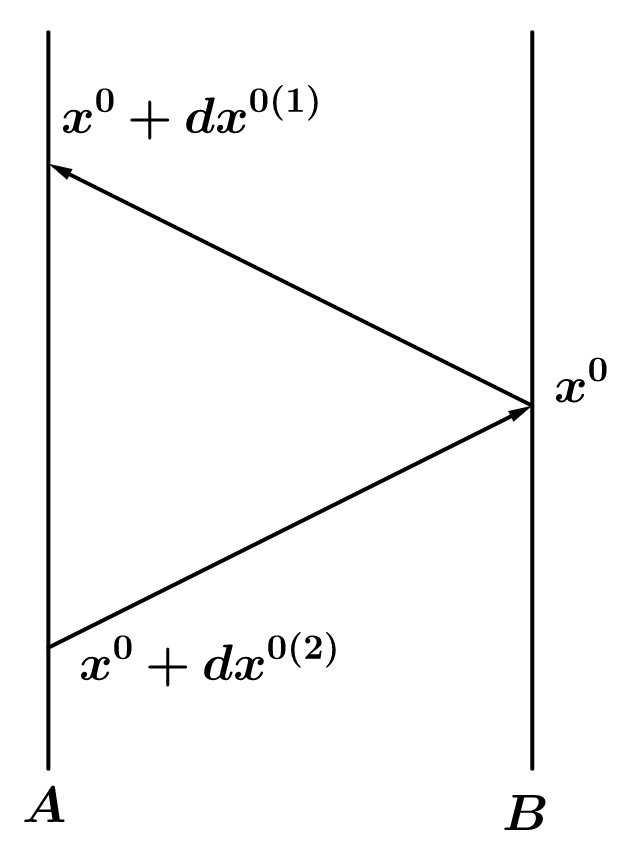
\includegraphics[width=5cm]{Imagenes/Fig17}
\caption[Medición de distancias en sistemas de coordenadas no inerciales.]{Representación esquemática del método de medición de distancias.}
\end{figure}
\begin{eqnarray}
\nonumber ds^{2}=&0&=g_{00}(dx^{0})^{2}+2g_{0i}dx^{0}dx^{i}+g_{ij}dx^{i}dx^{j}\\
\nonumber \Rightarrow dx^{o}&=&\left[-\frac{g_{oi}}{g_{00}}\pm\frac{\sqrt{g_{0i}g_{ok}+g_{00}g_{ik}}dx^{i}dx^{k}}{g_{00}}\right]\\
\Rightarrow dx^{0(2)}&=&\left[-\frac{g_{oi}}{g_{00}}+\frac{\sqrt{g_{0i}g_{ok}+g_{00}g_{ik}}dx^{i}dx^{k}}{g_{00}}\right]\\
\Rightarrow dx^{0(1)}&=&\left[-\frac{g_{oi}}{g_{00}}-\frac{\sqrt{g_{0i}g_{ok}+g_{00}g_{ik}}dx^{i}dx^{k}}{g_{00}}\right],
\end{eqnarray} 
ahora como $\triangle x^0=x^0+dx^{0(1)}-x^0-dx^{0(2)}$ tenemos:
\begin{equation}
\triangle x^0= -2\frac{\sqrt{g_{0i}g_{ok}+g_{00}g_{ik}}dx^{i}dx^{k}}{g_{00}}.
\end{equation}
Por otro lado:
\begin{equation}
dl=\frac{c}{2}\triangle\tau\ \text{y}\ \triangle\tau=\sqrt{-g_{00}}\triangle x^{0}\Rightarrow dl^{2}=\frac{c^{2}}{4}(-g_{00})(\triangle x^{0})^{2}=c^{2}\left(g_{ik}-\frac{g_{oi}g_{ok}}{g_{oo}}\right)dx^{i}dx^{k},
\end{equation}
con este resultado es posible analizar la estructura geométrica del espacio, para un disco que \textbf{no rota} tenemos que $\oint dl=2\pi r$, sin embargo en el caso que estamos estudiando la ecuación (3.158) nos lleva a:
\begin{eqnarray}
\nonumber dl^{2}&=&c^{2}\left(g_{22}-\frac{g_{o2}g_{o2}}{g_{oo}}\right)d\phi^{2},\ \text{para}\ \omega\ll 1\\
\nonumber &=& \left(r^{2}\frac{\frac{\omega^{2}r^{4}}{c^{2}}}{1-\frac{\omega^{2}r^{2}}{c^{2}}}\right)d\phi^{2}\approx \left(r^{2}+\frac{\omega^{2}r^{4}}{c^{2}}\left(1+\frac{\omega^{2}r^{2}}{c^{2}}\right)\right)d\phi^{2}\\
\nonumber &=& \approx r^{2}\left(1+\frac{\omega^{2}r^{2}}{c^{2}}\right)d\phi^{2}\\
\nonumber \Rightarrow dl &\approx &r \left(1+\frac{\omega^{2}r^{2}}{2c^{2}}\right)\\
\Rightarrow\oint dl&=& 2\pi r\left(1+\frac{\omega^{2}r^{2}}{2c^{2}}\right)>2\pi r,
\end{eqnarray}
el espacio es curvo!
\\
\\
Por último estudiemos el problema de la sincronización de relojes,observando la figura 3.1, un evento que es simultáneo en tiempo $x^0$ para $A$ sucede en $B$ justo en la mitad de los enventos de enviar y recibir la luz, es decir en $x^{0}+\frac{dx^{0(1)}+dx^{0(2)}}{2}=x^{0}-\frac{g_{oi}}{g_{00}}dx^{i}\equiv x^{0}+\triangle x^{0}$. En un sistema de referencia \textbf{sin rotación} $g_{oi}=0$ por tanto la sincronización es posible, sin embargo en nuestro caso $g_{0i}\neq 0\Rightarrow \triangle x^0\neq 0$, es por esto que al intentar sincronizar un reloj en una trayectoria cerrada vamos a fracasar debido a que al retornar al punto de partida el reloj 	va a haber acumulado un retraso $\triangle x^{0}=-\oint\frac{g_{oi}}{g_{oo}}dx^{i}$. Las consecuencias experimentales de este fenómeno fueron medidas por primera vez por Georges Sagnac, razón por la cual se conoce a este fenómeno como    \textbf{efecto Sagnac}.
\begin{figure}[h!]
\centering
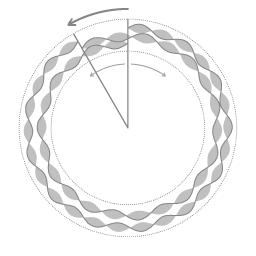
\includegraphics[width=7cm]{Imagenes/Fig18}
\caption[Representación esquemática del efecto Sagnac.]{Representación esquemática del efecto Sagnac, la interferencia se produce debido a la diferencia de camino óptico entre los haz.}
\end{figure}
\\
\\
El efecto Sagnac consiste en el corrimiento de las líneas del patrón de interferencia de dos haz de luz que viajan en direcciones opuestas en un interferómetro rotante, en la figura 3.2 se muestra un esquema del efecto. Calculemos el corrimiento, sabemos que:
\begin{equation}
\triangle t=\frac{1}{c}\triangle x^{0}=\frac{1}{c}\oint\frac{\frac{\omega r^{2}}{c}}{1-\frac{\omega^{2}r^{2}}{c^{2}}}d\phi\approx\frac{\omega}{c^{2}}\oint r^{2}d\phi=\frac{\omega2\pi r^{2}}{c^{2}},
\end{equation}
la discrepancia en tiempo propio para $\omega \ll 1$ es $\triangle \tau =\sqrt{-g_{00}}\triangle t\approx \triangle t$, con esto podemos calcular la longitud de camino óptico:
\begin{equation}
l+\triangle l=2\pi r+c\triangle \tau =L+\frac{2\omega \pi r^2}{c},
\end{equation}  
para el rayo que va en la dirección opuesta:
\begin{equation}
l-\triangle l=L-\frac{2\omega \pi r^2}{c}.
\end{equation}
Por tanto la diferencia de camino óptico es $\frac{4\omega \pi r^2}{c}$, lo que corresponde a un corrimiento:
\begin{equation}
\triangle N= \frac{4\pi r^2\omega}{c\lambda}.
\end{equation}
En el experimento realizado por Sagnac $\omega=14\text{rad/s},\ \pi r^2=0.0863 m^2\ \text{y}\ \lambda=0.436\times10^{-6}m$, al insertar estos datos en (3.163) obtenemos:
\begin{equation}
\triangle N=0.036\ ,
\end{equation}
valor que concuerda con el experimento.
\subsection{El propagador.}
En esta última sección vamos a derivar el propagador para una partícula que se mueve en una trayectoria circular en un espacio-tiempo rotante, como ya hemos visto, en este tipo de sistemas de coordenadas aparecen efectos nuevos, como el efecto Sagnac. Esto último debido a que son sistemas de coordenadas no inerciales, es por esta razón que resulta interesante estudiar este problema desde un punto de vista cuántico.
\\
\\
Para un espacio-tiempo (1+2) dimensional, rotante (con velocidad angular $\omega$), la métrica esta dada por:
\begin{equation}
g_{\mu\nu}=\left(\begin{array}{ccc}
(1-r^{2}\omega^{2}) & 0 & -r^{2}\omega\\
0 & -1 & 0\\
-r^{2}\omega & 0 & -r^{2}
\end{array}\right),
\end{equation}
notemos que hemos cambiado la signatura de la mética a $(-,+,+)$ y de ahora en adelante usaremos unidades naturales $(\hbar=c=G=1)$. Si calculamos el determinante de la ecuación (3.165) obtenemos:
\begin{equation}
\det g_{\mu\nu}=r^{2}\Rightarrow g=\sqrt{\det g_{\mu\nu}}=r,
\end{equation}
este es el mismo resultado que obtendriamos para el caso del espacio de Minkowski en coordenadas polares, por tanto, el espacio-tiempo sigue siendo plano. Una partícula relativista de masa $\mu$, espín cero y que se mueve en un espacio-tiempo curvo obedece la ecuación de Klein-Gordon en espacio curvo:
\begin{equation}
\left(\square-\frac{\mathcal{R}}{8}-\mu^{2}\right)\psi=0\ ;\ \square=g^{\mu\nu}\nabla_{\mu}\nabla_{\nu},
\end{equation} 
donde $\mathcal{R}$ es el escalar de Ricci. El propagador para esta partícula es:
\begin{equation}
K(t^{'},t^{''},r^{'},r^{''},\theta^{'}.\theta^{''})=\int\exp(iS)\mathcal{D}[x],
\end{equation}
donde
\begin{equation}
S=\int_{0}^{\Lambda}\left[\frac{1}{2}g_{\mu\nu}\dot{x}^{\mu}\dot{x}^{\nu}-k^{2}\right]d\lambda\ ;\ k^{2}=\frac{1}{2}\left[-\frac{1}{24}\mathcal{R}+\mu^{2}\right].	
\end{equation}
Sabemos de las secciones anteriores que el término proporcional al escalar de Ricci en la ecuación (3.169) viene del hecho de llevar a cabo el cálculo de la integral de trayectoria en espacio-tiempo curvo, sin embargo, como consecuencia directa de la ecuación (3.166) (el espacio-tiempo es plano), entonces $\mathcal{R}=0$. Tomando en cuenta todo lo anterior:
\begin{equation}
S=\int_{0}^{\Lambda}\left[-\frac{1}{2}\dot{t}^{2}(1-\omega^{2}r^{2})+\frac{\dot{r}^{2}}{2}+\frac{r^{2}\dot{\theta}^{2}}{2}+r^{2}\omega\dot{\theta}\dot{t}-\frac{\mu^{2}}{2}\right]d\lambda.
\end{equation} 
En la expresión anterior hemos usado la notación $\dot{x}\equiv\frac{dx}{d\lambda}$, si escribimos el propagador (3.168) en forma discretizada:
\begin{equation}
K(t^{'},t^{''},r^{'},r^{''},\theta^{'}.\theta^{''})=\lim_{N\to\infty}\int\prod_{j=1}^{N}\exp(iS_{j})\mathcal{D}[x],
\end{equation}
donde:
\begin{equation}
\mathcal{D}[x]=\lim_{N\to\infty}\prod_{j=1}^{N}\left(\frac{1}{2\pi i\epsilon_{j}}\right)^{\frac{3}{2}}\prod_{j=1}^{N-1}g_{j}^{\frac{1}{2}}dt_{j}dr_{j}d\theta_{j}=\lim_{N\to\infty}\prod_{j=1}^{N}\left(\frac{1}{2\pi i\epsilon_{j}}\right)^{\frac{3}{2}}\prod_{j=1}^{N-1}r_{j}dt_{j}dr_{j}d\theta_{j},
\end{equation}
y
\begin{equation}
S_{j}=-\frac{1}{2}(1-\omega^{2}r_{j}^{2})\frac{(\triangle t_{j})^{2}}{\epsilon_{j}}+\frac{(\triangle r_{j})^{2}}{2\epsilon_{j}}+r_{j}^{2}\frac{(\triangle\theta_{j})^{2}}{2\epsilon_{j}}+r_{j}^{2}\omega\frac{\triangle\theta_{j}\triangle t_{j}}{\epsilon_{j}}-\frac{\mu^{2}\epsilon_{j}}{2}.
\end{equation}
Podemos fijar la variable radial a un valor $r=R$, mediante la siguiente relación:
\begin{equation}
\left(\frac{1}{2\pi i\epsilon_{j}}\right)^{\frac{1}{2}}\exp\left(\frac{i(\triangle r_{j})^{2}}{2\epsilon_{j}}\right)=\delta(r_{j}-r_{j-1}),
\end{equation}
por tanto el propagador queda:
\begin{equation}
K(t^{'},t^{''},\theta^{'}.\theta^{''})=\exp\left(-\frac{i\mu^{2}\Lambda}{2}\right)\lim_{N\to\infty}\int\prod_{j=1}^{N}\exp(iS_{j}(t,\theta))\prod_{j=1}^{N}\left(\frac{1}{2\pi i\epsilon_{j}}\right)\prod_{j=1}^{N-1}Rdt_{j}d\theta_{j},
\end{equation}
con
\begin{equation}
S_{j}(t,\theta)=-\frac{1}{2}(1-\omega^{2}R^{2})\frac{(\triangle t_{j})^{2}}{\epsilon_{j}}+R^{2}\frac{(\triangle\theta_{j})^{2}}{2\epsilon_{j}}+R^{2}\omega\frac{\triangle\theta_{j}\triangle t_{j}}{\epsilon_{j}}.
\end{equation}
Si introducimos la variable temporal adimensional $\triangle t_j\omega =\triangle \tau_j$, obtenemos:
\begin{equation}
S_{j}(\tau,\theta)=-\frac{1}{2\epsilon_{j}}\left(\frac{1}{\omega^{2}}-R^{2}\right)(\triangle\tau_{j})^{2}+R^{2}\frac{(\triangle\theta_{j})^{2}}{2\epsilon_{j}}+R^{2}\frac{\triangle\theta_{j}\triangle\tau_{j}}{\epsilon_{j}},
\end{equation}
y el propagador queda escrito como:
\begin{equation}
K(\tau^{'},\tau^{''},\theta^{'},\theta^{''})=\exp\left(-\frac{i\mu^{2}\Lambda}{2}\right)\lim_{N\to\infty}\int\prod_{j=1}^{N}\exp(iS_{j}(\tau,\theta))\prod_{j=1}^{N}\left(\frac{1}{2\pi i\epsilon_{j}}\right)\prod_{j=1}^{N-1}\frac{R}{\omega}d\tau_{j}d\theta_{j}.
\end{equation}
Ahora con el fin de eliminar el término proporcional a $\triangle \theta_j\triangle \tau_j$, es decir separar de nuevo las coordenadas, hagamos una rotación de las mismas. Si se tiene una forma cuadrática $F=Ax^2+Bxy+Cy^2$, podemos hacer una rotación de tal manera que es posible escribir $F=A^{'}x^{'2}+C^{'}y^{'2}$, para que esto se cumpla debemos tener que $\cot (2\phi)=\frac{A-C}{B}$, en este caso el término $xy$ se anula y tenemos que:
\begin{align}
\nonumber A^{'}&=A\cos^{2}\phi+B\sin\phi\cos\phi+C\sin^{2}\phi\\
B^{'}&=A\sin^{2}\phi-B\sin\phi\cos\phi+C\cos^{2}\phi.
\end{align}
Observando la ecuación (3.177), en nuestro caso:
\begin{equation}
A=-\frac{1}{2\epsilon_{j}}\left(\frac{1}{\omega^{2}}-R^{2}\right),\ B=\frac{R^{2}}{\epsilon_{j}},\ C=\frac{R^{2}}{2\epsilon_{j}},
\end{equation}
así:
\begin{equation}
\cot(2\phi)=-\frac{1}{2R^{2}\omega^{2}}.
\end{equation}
Acudiendo a la Figura 3.3, escribimos las siguientes relaciones:
\begin{figure}[h!]
\centering
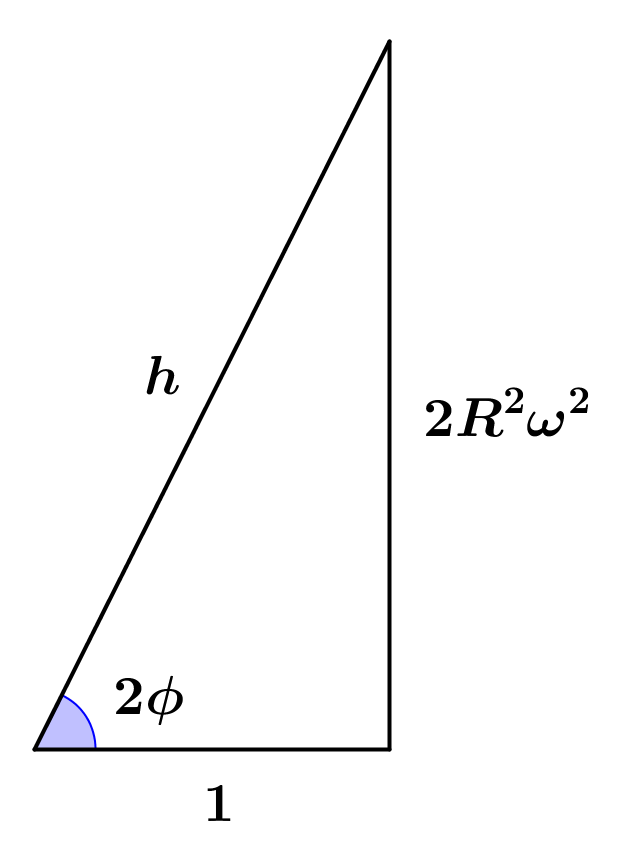
\includegraphics[width=3.8cm]{Imagenes/Fig19}
\caption[Triángulo de funciones trigonométricas.]{Triángulo para la construcción de funciones trigonométricas.}
\end{figure}
\begin{align}
\nonumber h&=\sqrt{1+4R^4\omega^4}\\
\nonumber \cos(2\phi)&=-\frac{1}{h}\\
\nonumber \sin\phi&=\sqrt{\frac{1-\cos2\phi}{2}}=\sqrt{\frac{h+1}{2h}}\\
\nonumber \cos\phi&=\sqrt{\frac{1+\cos2\phi}{2}}=\sqrt{\frac{h-1}{2h}}\\
\sin\phi\cos\phi&=\frac{R^{2}\omega^{2}}{h}.
\end{align}
Combinando las ecuaciones (3.179) y (3.182), obtenemos:
\begin{align}
\nonumber A^{'}&=\frac{1}{2\epsilon_{j}}\left[R^{2}+\frac{1}{2h\omega^{2}}-\frac{1}{2\omega^{2}}+\frac{2R^{4}\omega^{2}}{h}\right]\\
C^{'}&=\frac{1}{2\epsilon_{j}}\left[R^{2}-\frac{1}{2h\omega^{2}}-\frac{1}{2\omega^{2}}-\frac{2R^{4}\omega^{2}}{h}\right],
\end{align}
por tanto:
\begin{equation}
K(\bar{\tau}^{'},\bar{\tau}^{''},\bar{\theta}^{'},\bar{\theta}^{''})=\exp\left(-\frac{i\mu^{2}\Lambda}{2}\right)\lim_{N\to\infty}\int\prod_{j=1}^{N}\exp(iS_{j}(\bar{\tau},\bar{\theta}))\prod_{j=1}^{N}\left(\frac{1}{2\pi i\epsilon_{j}}\right)\prod_{j=1}^{N-1}\frac{R}{\omega}d\bar{\tau}_{j}d\bar{\theta}_{j},
\end{equation}
donde
\begin{equation}
S_{j}(\bar{\tau},\bar{\theta})=A^{'}(\triangle\bar{\tau}_{j})^{2}+C^{'}(\triangle\bar{\theta}_{j})^{2}.
\end{equation}
En estas últimas dos expresiones hemos denotado las coordenadas rotadas como $\bar{\tau},\bar{\theta}$ y debido a que la transformación es una rotación, los diferenciales no se premultiplican por ningún factor debido a que $\det J=1$. Si escribimos:
\begin{equation}
S_{j}(\bar{\tau},\bar{\theta})=\left(\frac{1}{2\epsilon_{j}}\right)\alpha(\triangle\bar{\tau}_{j})^{2}+\left(\frac{1}{2\epsilon_{j}}\right)\beta(\triangle\bar{\theta}_{j})^{2},
\end{equation}
con
\begin{equation}
\alpha=\left[R^{2}+\frac{1}{2h\omega^{2}}-\frac{1}{2\omega^{2}}+\frac{2R^{4}\omega^{2}}{h}\right],\ \beta=\left[R^{2}-\frac{1}{2h\omega^{2}}-\frac{1}{2\omega^{2}}-\frac{2R^{4}\omega^{2}}{h}\right].
\end{equation}
Si ahora $T_j=\frac{1}{\omega}\bar{\tau}_j$ y $R\bar{\theta}_j=\Theta_j$, tenemos que la ecuación (3.184) se transforma en:
\begin{equation}
K(T^{'},T^{''},\Theta^{'},\Theta^{''})=\exp\left(-\frac{i\mu^{2}\Lambda}{2}\right)\lim_{N\to\infty}\int\prod_{j=1}^{N}\exp(iS_{j}(T,\Theta))\prod_{j=1}^{N}\left(\frac{1}{2\pi i\epsilon_{j}}\right)\prod_{j=1}^{N-1}dT_{j}d\Theta_{j},
\end{equation}
donde:
\begin{eqnarray}
\nonumber &S_{j}(T,\Theta)=\left(\frac{1}{2\epsilon_{j}}\right)\alpha^{'}(\triangle T_{j})^{2}+\left(\frac{1}{2\epsilon_{j}}\right)\beta^{'}(\triangle\Theta_{j})^{2}&\\
&\alpha^{'}=\left[R^{2}\omega^{2}+\frac{1}{2h}-\frac{1}{2}+\frac{2R^{4}\omega^{4}}{h}\right],\ \beta^{'}=\left[1-\frac{1}{2hR^{2}\omega^{2}}-\frac{1}{2R^{2}\omega^{2}}-\frac{2R^{2}\omega^{2}}{h}\right]&.
\end{eqnarray}
Después de toda la manipulación que hemos hecho a la expresión (3.175), hasta llevarla a (3.188), por fin hemos logrado obtener una forma funcional como la que ya hemos integrado en la sección $\mathsection$2.1.1, en general el resultado que descubrimos en esa sección se puede escribir como:
\begin{equation}
\lim_{N\to\infty}\int\prod_{j=1}^{N}\exp\left(\frac{ia(\triangle x_{j})^{2}}{2\epsilon_{j}}\right)\prod_{j=1}^{N}\left(\frac{1}{2\pi i\epsilon_{j}}\right)^{\frac{1}{2}}\prod_{j=1}^{N-1}dx_{j}=\left(\frac{A}{2\pi i\Lambda}\right)^{\frac{1}{2}}\exp\left(\frac{iA}{2\Lambda}(x_{N}-x_{0})^{2}\right),
\end{equation}
usando este resultado en (3.188) obtenemos:
\begin{equation}
K(T^{'},T^{''},\Theta^{'},\Theta^{''})=\exp\left(-\frac{i\mu^{2}\Lambda}{2}\right)\left(\frac{\alpha^{'}\beta^{'}}{(2\pi i\Lambda)^{2}}\right)^{\frac{1}{2}}\exp\left(\frac{i\alpha^{'}}{2\Lambda}(T_{N}-T_{0})^{2}\right)\exp\left(\frac{i\beta^{'}}{2\Lambda}(\Theta{}_{N}-\Theta_{0})^{2}\right).
\end{equation}
Para finalizar debemos devolver todas las transformaciones que hemos realizado, primero $T\to\frac{1}{\omega}\bar{\tau}$ y $\Theta\to R\bar{\theta}$, por tanto:
\begin{equation}
K(\bar{\tau}^{'},\bar{\tau}^{''},\bar{\theta}^{'},\bar{\theta}^{''})=\exp\left(-\frac{i\mu^{2}\Lambda}{2}\right)\left(\frac{\alpha\beta\omega^2}{(2\pi i\Lambda)^{2}R^2}\right)^{\frac{1}{2}}\exp\left(\frac{i\alpha}{2\Lambda}(\bar{\tau}^{''}-\bar{\tau}^{'})^{2}\right)\exp\left(\frac{i\beta}{2\Lambda}(\bar{\theta}^{''}-\bar{\theta}^{'})^{2}\right),
\end{equation}
notemos que en la expresión (3.192) ya no usamos $\alpha^{'},\beta^{'}$, sino $\alpha,\beta$. La rotación que realizamos se puede escribir como:
\begin{eqnarray}
\nonumber \bar{\tau}&=\tau\cos\phi+\theta\sin\phi\Rightarrow\bar{\tau}^{2}=\tau^{2}\cos^{2}\phi+\tau\theta2\sin\phi\cos\phi+\theta^{2}\sin^{2}\phi\\
\bar{\theta}&=-\tau\sin\phi+\theta\cos\phi\Rightarrow\bar{\theta}^{2}=\tau^{2}\sin^{2}\phi-\tau\theta2\sin\phi\cos\phi+\theta^{2}\cos^{2}\phi ,
\end{eqnarray} 
así podemos escribir:
\begin{eqnarray}
\nonumber K(\tau^{'},\tau^{''},\theta^{'},\theta^{''})&\propto &\exp\left(\frac{i}{2\Lambda}\left[(\tau^{''}-\tau^{'})^{2}(\alpha\cos^{2}\phi+\beta\sin^{2}\phi)+(\theta^{''}-\theta^{''})^{2}(\alpha\sin^{2}\phi+\beta\cos^{2}\phi)\right]\right)\\
\nonumber &\times & \exp\left(\frac{i}{2\Lambda}\left[(\tau^{''}-\tau^{'})(\theta^{''}-\theta^{''})2\sin\phi\cos\phi(\alpha-\beta)\right]\right)\\
\nonumber &\propto & \exp\left(\frac{i}{2\Lambda}\frac{(\tau^{''}-\tau^{'})^{2}}{2}\left[R^{2}-\frac{1}{2\omega^{2}}-\frac{1}{2\omega^{2}h^{2}}-\frac{2R^{4}\omega^{2}}{h^{2}}\right]\right)\\
\nonumber &\times & \exp\left(\frac{i}{2\Lambda}\frac{(\theta^{''}-\theta^{''})^{2}}{2}\left[R^{2}-\frac{1}{2\omega^{2}}+\frac{1}{2\omega^{2}h^{2}}+\frac{2R^{4}\omega^{2}}{h^{2}}\right]\right)\\
&\times & \exp\left(\frac{i}{2\Lambda}(\tau^{''}-\tau^{'})(\theta^{''}-\theta^{''})\frac{2R^{2}\omega^{2}}{h^{2}}\left[\frac{1}{\omega^{2}}+4R^{4}\omega^{2}\right]\right).
\end{eqnarray}
Finalmente si hacemos la última sustitución, $\tau \to \omega t$:
\begin{eqnarray}
\nonumber K(t^{'},t^{''},\theta^{'},\theta^{''})&=&\exp\left(-\frac{i\mu^{2}\Lambda}{2}\right)\left(\frac{\alpha\beta\omega^2}{(2\pi i\Lambda)^{2}R^2}\right)^{\frac{1}{2}}\exp\left(\frac{i}{2\Lambda}\frac{(t^{''}-t^{'})^{2}}{2}\left[R^{2}\omega^{2}-\frac{1}{2}-\frac{1}{2h^{2}}-\frac{2R^{4}\omega^{4}}{h^{2}}\right]\right)\\
\nonumber &\times & \exp\left(\frac{i}{2\Lambda}\frac{(\theta^{''}-\theta^{'})^{2}}{2}\left[R^{2}-\frac{1}{2\omega^{2}}+\frac{1}{2\omega^{2}h^{2}}+\frac{2R^{4}\omega^{2}}{h^{2}}\right]\right)\\
&\times &\exp\left(\frac{i}{2\Lambda}(t^{''}-t^{'})(\theta^{''}-\theta^{'})\left[\frac{2R^{2}\omega}{h^{2}}+\frac{8R^{6}\omega^{5}}{h^{2}}\right]\right),
\end{eqnarray} 
una forma de realizar una prueba de consistencia al resultado (3.195) es explorar el límite $\omega \to 0$, si tomamos este límite en (3.195) vemos que:
\begin{equation}
K(t^{'},t^{''},\theta^{'},\theta^{''})_{\omega\to0}=\exp\left(-\frac{i\mu^{2}\Lambda}{2}\right)\left(\frac{1}{2\pi\Lambda}\right)\exp\left(\frac{i}{2\Lambda}\left[-\frac{(t^{''}-t^{'})^{2}}{2}+\frac{(\theta^{''}-\theta^{''})^{2}}{2}R^{2}\right]\right).
\end{equation} 
Esto debido a que $\lim_{\omega\to 0}\left(\alpha\beta\frac{\omega^2}{R^2}\right)^{\frac{1}{2}}=i$, vemos que la expresión (3.196) tiene las coordenadas desacopladas y no depende de $\omega$, esto era lo esperado.

\subsection{Patrón de interferencia.}
Como vimos en la $\mathsection$ 2, ecuación (2.3), la amplitud cuántica de probabilidad se puede calcular como el módulo cuadrado del propagador:
\begin{equation}
P(x)=|K(x)|^{2},
\end{equation}
en nuestra versión del efecto Sagnac consideramos dos partículas que viajan en direcciones opuestas y siguen trayectorias circulares. El propagador para este sistema se puede escribir como:
\begin{equation}
K_{T}(t,\theta)=K(t,\theta)+K(t,-\theta),
\end{equation}
esto se puede ver debido a que su suponemos que las partículas dejan la fuente emisora al mismo tiempo y con la misma velocidad, cuando una de ellas tenga una posición angular $\theta$, la otra tendrá una posición angular opuesta correspondiente a $-\theta$. Esto se ilustra en la figura 3.4.
\begin{figure}[h!]
\centering
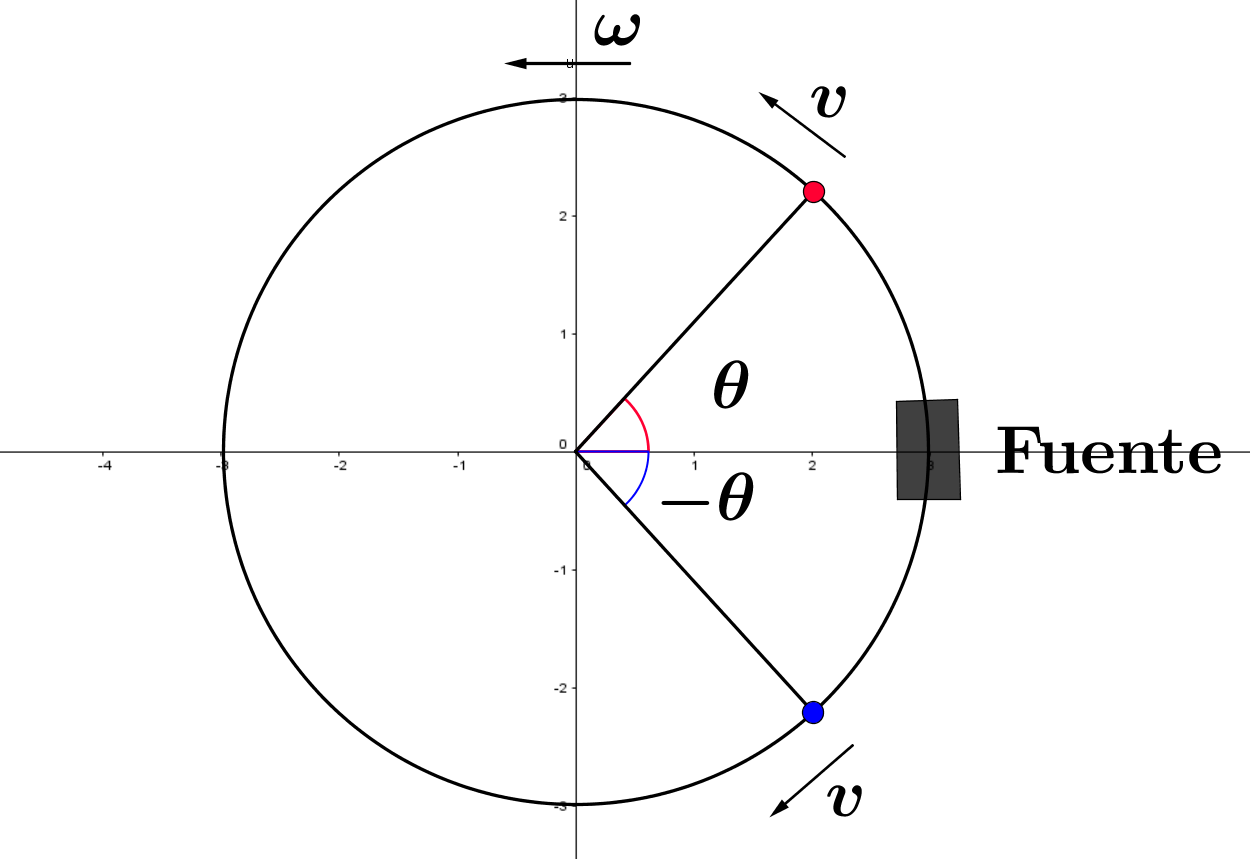
\includegraphics[width=10cm]{Imagenes/Fig20}
\caption[Justificación esquemática del propagador.]{En esta figura se aprecia el hecho de que las partículas que viajan en direcciones contrarias, tienen posiciones angulares opuestas.}
\end{figure}
Ya sabemos de la sección anterior que el propagador para una de las partículas esta dado por la ecuación (3.195), si consideramos un viajero no masivo ($\mu=0$), entonces:
\begin{equation}
K(t^{'},t^{''},\theta^{'},\theta^{''})=A\exp\left[\frac{i}{2\Lambda}\frac{t^{2}}{2}a\right]\exp\left[\frac{i}{2\Lambda}\frac{\theta^{2}}{2}b\right]\exp\left[\frac{i}{2\Lambda}\theta tc\right],
\end{equation}
con
\begin{eqnarray}
\nonumber &A=\frac{(\alpha\beta)^{\frac{1}{2}}\omega}{2\pi i\Lambda R}\ ,\ t=t^{''}-t^{'}\ ,\ \theta=\theta^{''}-\theta^{'},&\\
\nonumber & a=\left[R^{2}\omega^{2}-\frac{1}{2}-\frac{1}{2h^{2}}-\frac{2R^{4}\omega^{4}}{h^{2}}\right]\ ,\ b=\left[R^{2}-\frac{1}{2\omega^{2}}+\frac{1}{2\omega^{2}h^{2}}+\frac{2R^{4}\omega^{2}}{h^{2}}\right],&\\
&c=\left[\frac{2R^{2}\omega}{h^{2}}+\frac{8R^{6}\omega^{5}}{h^{2}}\right].&
\end{eqnarray}
Por tanto,
\begin{eqnarray}
\nonumber K_T(t,\theta)&=&A\exp\left[\frac{i}{2\Lambda}\frac{t^{2}}{2}a\right]\exp\left[\frac{i}{2\Lambda}\frac{\theta^{2}}{2}b\right]\exp\left[\frac{i}{2\Lambda}\theta tc\right]\\
\nonumber &+&A\exp\left[\frac{i}{2\Lambda}\frac{t^{2}}{2}a\right]\exp\left[\frac{i}{2\Lambda}\frac{(-\theta)^{2}}{2}b\right]\exp\left[\frac{i}{2\Lambda}(-\theta)tc\right]\\
&=&A\exp\left[\frac{i}{2\Lambda}\frac{t^{2}}{2}a\right]\exp\left[\frac{i}{2\Lambda}\frac{\theta^{2}}{2}b\right]\left[\exp\left[\frac{i}{2\Lambda}\theta tc\right]+\exp\left[-\frac{i}{2\Lambda}\theta tc\right]\right],
\end{eqnarray}
así, si calculamos $|K_T(t,\theta)|^2$:
\begin{equation}
|K_{T}(t,\theta)|^{2}=AA^{*}\left[\exp\left[\frac{i}{2\Lambda}\theta tc\right]+\exp\left[-\frac{i}{2\Lambda}\theta tc\right]\right]\left[\exp\left[-\frac{i}{2\Lambda}\theta tc\right]+\exp\left[\frac{i}{2\Lambda}\theta tc\right]\right],
\end{equation}
usando el hecho de que $2\cos\theta=e^{i\theta}+e^{-i\theta}$, tenemos que:
\begin{equation}
|K_{T}(t,\theta)|^{2}=4AA^{*}\cos^{2}\left(\frac{\theta tc}{2\Lambda}\right).
\end{equation}
Ahora para $\omega\ll 1$ tenemos que el tiempo propio y el tiempo coordenado son muy parecidos, así $\frac{t}{\Lambda}\approx 1$, entonces:
\begin{equation}
|K_{T}(t,\theta)|^{2}=4AA^{*}\cos^{2}\left(\frac{\theta c}{2}\right),
\end{equation}
por último:
\begin{eqnarray}
\nonumber c&=&\left[\frac{2R^{2}\omega}{h^{2}}+\frac{8R^{6}\omega^{5}}{h^{2}}\right]\\
\nonumber c&\approx &  2R^{2}\omega(1-4R^{4}\omega^{4})\approx2R^{2}\omega .
\end{eqnarray}
Así 
\begin{equation}
P(\theta)=|K_{T}(\theta)|^{2}=4AA^{*}\cos^{2}(R^{2}\omega\theta),
\end{equation}
si analizamos la interferencia luego de que las partículas hayan dado una vuelta completa $\theta=\theta^{''}-\theta^{'}=2\pi$, entonces:
\begin{equation}
P(2\pi)=|K_{T}(2\pi)|^{2}=4AA^{*}\cos^{2}(2\pi R^{2}\omega).
\end{equation}
Si restauramos las unidades del sistema internacional:
\begin{equation}
P(2\pi)=4AA^{*}\cos^{2}\left(\frac{2\pi R^{2}\omega}{\hbar c^{2}}\right),
\end{equation}
y usando las relaciones (en el caso de partículas no masivas), $E=pc,\ p=\frac{h}{\lambda},\ \hbar=\frac{h}{2\pi},\ c=\lambda \nu$, obtenemos:
\begin{equation}
P(2\pi)\propto\cos^{2}\left(\frac{4\pi^{2}R^{2}\omega}{\lambda c}\right).
\end{equation}
Por otro lado de la óptica ondulatoria, sabemos que dos ondas monocromáticas de longitud de onda $\lambda$ 	y que poseen una diferencia de camino óptico $\triangle l$, forman un patrón de interferencia con una intesidad proporcional a [22]:
\begin{equation}
P(\triangle l)\propto\cos^{2}\left(\frac{\pi\triangle l}{\lambda}\right),
\end{equation} 
retomando el resultado que derivamos en la $\mathsection$ 3.5.1, ecuación (3.162):
\begin{equation}
\triangle l=\frac{4\pi R^{2}\omega}{c}\Rightarrow P(2\pi)\propto\cos^{2}\left(\frac{4\pi^{2}R^{2}\omega}{\lambda c}\right).
\end{equation}
Por tanto comparando la ecuación (3.208) y (3.210) vemos que hay consistencia en los dos tipos de aproximaciones, por lo menos a primer orden en $\omega$. Una de estas aproxiciones es puramente clásica en contraste con el método de integrales de trayectoria, que considera los aspectos cuánticos del problema. Finalmente otra ventaja de la aproximación por integrales de trayectoria es que si de entrada permitimos que entren términos de mayor orden en la expansión, tendrémos "correciones" cuánticas al resultado clásico que hemos esbozado en la $\mathsection$ 3.5.1 . 
 




 % Experimental Setup

\chapter{Bibliografía.}
\begin{itemize}
\item[[1]] C. Cohen-Tannudji, B. Diu ;\textit{Quantum Mechanics, Volume One}; Wiley, New-York, (1991).
\item[[2]] Mathieu Beau; \textit{Feynman Integral and one/two slits electrons diffraction : an analytic study}; \texttt{arXiv:1110.2346v3}.
\item[[3]]  L.D. Faddeev,  V.N. Popov ;\textit{Feynman diagrams for the Yang-Mills field}; Physics Letters B Volume 25, Issue 1, 24 July 1967, Pages 29-30.
\item[[4]] Lewis H. Ryder;\textit{Quantum Field Theory};Second Edition (1996) 
\item[[5]] M Nakahara;\textit{Geometry, Topology and Physics};Second Edition (2003) 
\item[[6]]  C.N Yang,  R.L Mills ;\textit{Conservation of Isotopic Spin and Isotopic Gauge Invariance}; Phys. Rev. 96, 191 – Published 1 October 1954.
\item[[7]]  Hermann Weyl;\textit{Elektron und Gravitation. I}; Zeitschrift für Physik, May 1929, Volume 56, Issue 5, pp 330-352.
\item[[8]] R.M. Wald.;\textit{General Relativity.};University of Chicago Press, (1984). 
\item[[9]]  Bryce DeWitt;\textit{Dynamical Theory in Curved Spaces. I. A Review of the Classical and Quantum Action Principles.}; Reviews of Modern Physics, July 1957 .
\item[[9]]  Bryce DeWitt;\textit{Dynamical Theory in Curved Spaces. I. A Review of the Classical and Quantum Action Principles.}; Reviews of Modern Physics, July 1957 .
\item[[10]]  Christian Grosche;\textit{AN INTRODUCTION INTO
THE FEYNMAN PATH INTEGRAL.}; arXiv:hep-th/9302097v1 20 Feb 1993 .
\item[[11]]  . Duru and H. Kleinert;\textit{Solution of the Path Integral for the H-Atom.}; Phys. Letters B 84, 185 (1979).
\item[[12]]  . Duru and H. Kleinert;\textit{Quantum Mechanics of H-Atom from Path Integrals.};  Fortschr. d. Phys. 30, 401 (1982).
\item[[13]]  Hagen Kleinert;\textit{Path Integrals in Quantum Mechanics, Statistics, Polymer Physics, and Financial Markets.};  World Scientific, Singapore 2009.
\item[[14]]  M Chaichian and A Demichev;\textit{Path Integrals in Physics, Volume I
Stochastic Processes and Quantum Mechanics.};  IOP Publishing Ltd 2001.
\item[[15]] Dennis V. Perepelitsa;\textit{Path Integrals in Quantum Mechanics.};\texttt{http://goo.gl/y29SeM}.

\end{itemize}
 % Experiment 1

%\chapter*{Bibliografía.}
\begin{itemize}
\item[[1]] Lewis Ryder ;\textit{Introduction to General Relativity.};Cambridge University Press (2009).
\item[[2]] Steven Weinberg ;\textit{The Quantum Theory of Fields, Volume I-II.};Cambridge University Press (1995).
\item[[3]] Daniel Baumann;\textit{TASI Lectures on Inflation.};\texttt{https://arxiv.org/pdf/0907.5424v2.pdf}.
\item[[4]] C. Cohen-Tannudji, B. Diu ;\textit{Quantum Mechanics, Volume One}; Wiley, New-York, (1991).
\item[[5]] Mathieu Beau; \textit{Feynman Integral and one/two slits electrons diffraction : an analytic study}; \texttt{arXiv:1110.2346v3}.
\item[[6]]  L.D. Faddeev,  V.N. Popov ;\textit{Feynman diagrams for the Yang-Mills field}; Physics Letters B Volume 25, Issue 1, 24 July 1967, Pages 29-30.
\item[[7]] Lewis H. Ryder;\textit{Quantum Field Theory};Second Edition (1996) 
\item[[8]] M Nakahara;\textit{Geometry, Topology and Physics};Second Edition (2003) 
\item[[9]]  C.N Yang,  R.L Mills ;\textit{Conservation of Isotopic Spin and Isotopic Gauge Invariance}; Phys. Rev. 96, 191 – Published 1 October 1954.
\item[[10]]  Hermann Weyl;\textit{Elektron und Gravitation. I}; Zeitschrift für Physik, May 1929, Volume 56, Issue 5, pp 330-352.
\item[[11]] R.M. Wald.;\textit{General Relativity.};University of Chicago Press, (1984). 
\item[[12]]  Bryce DeWitt;\textit{Dynamical Theory in Curved Spaces. I. A Review of the Classical and Quantum Action Principles.}; Reviews of Modern Physics, July 1957 .
\item[[13]]  Christian Grosche;\textit{AN INTRODUCTION INTO
THE FEYNMAN PATH INTEGRAL.}; arXiv:hep-th/9302097v1 20 Feb 1993 .
\item[[14]]  . Duru and H. Kleinert;\textit{Solution of the Path Integral for the H-Atom.}; Phys. Letters B 84, 185 (1979).
\item[[15]]  . Duru and H. Kleinert;\textit{Quantum Mechanics of H-Atom from Path Integrals.};  Fortschr. d. Phys. 30, 401 (1982).
\item[[16]]  Hagen Kleinert;\textit{Path Integrals in Quantum Mechanics, Statistics, Polymer Physics, and Financial Markets.};  World Scientific, Singapore 2009.
\item[[17]]  M Chaichian and A Demichev;\textit{Path Integrals in Physics, Volume I
Stochastic Processes and Quantum Mechanics.};  IOP Publishing Ltd 2001.
\item[[18]] Dennis V. Perepelitsa;\textit{Path Integrals in Quantum Mechanics.};\texttt{http://goo.gl/y29SeM}.
\item[[19]] Sagnac, Georges;\textit{L'éther lumineux démontré par l'effet du vent relatif d'éther dans un interféromètre en rotation uniforme.}; Comptes Rendus 157: 708–710.
\item[[20]] Sagnac, Georges;\textit{Sur la preuve de la réalité de l'éther lumineux par l'expérience de l'interférographe tournant.};  Comptes Rendus 157: 1410–1413.
\item[[21]] Guido Rizzi, Matteo Luca Ruggiero ;\textit{Path Integrals in Quantum Mechanics.};Springer Science+Business Media Dordrecht (2004).
\item[[22]] Hector Alzate ;\textit{Física de las ondas.}; Univerisad de Antioquia (2007).
\end{itemize}
 % Experiment 2

%\input{Chapters/Chapter6} % Results and Discussion

%\input{Chapters/Chapter7} % Conclusion

%% ----------------------------------------------------------------
% Now begin the Appendices, including them as separate files

\addtocontents{toc}{\vspace{2em}} % Add a gap in the Contents, for aesthetics

\appendix % Cue to tell LaTeX that the following 'chapters' are Appendices

%\chapter{An Appendix}

Lorem ipsum dolor sit amet, consectetur adipiscing elit. Vivamus at pulvinar nisi. Phasellus hendrerit, diam placerat interdum iaculis, mauris justo cursus risus, in viverra purus eros at ligula. Ut metus justo, consequat a tristique posuere, laoreet nec nibh. Etiam et scelerisque mauris. Phasellus vel massa magna. Ut non neque id tortor pharetra bibendum vitae sit amet nisi. Duis nec quam quam, sed euismod justo. Pellentesque eu tellus vitae ante tempus malesuada. Nunc accumsan, quam in congue consequat, lectus lectus dapibus erat, id aliquet urna neque at massa. Nulla facilisi. Morbi ullamcorper eleifend posuere. Donec libero leo, faucibus nec bibendum at, mattis et urna. Proin consectetur, nunc ut imperdiet lobortis, magna neque tincidunt lectus, id iaculis nisi justo id nibh. Pellentesque vel sem in erat vulputate faucibus molestie ut lorem.

Quisque tristique urna in lorem laoreet at laoreet quam congue. Donec dolor turpis, blandit non imperdiet aliquet, blandit et felis. In lorem nisi, pretium sit amet vestibulum sed, tempus et sem. Proin non ante turpis. Nulla imperdiet fringilla convallis. Vivamus vel bibendum nisl. Pellentesque justo lectus, molestie vel luctus sed, lobortis in libero. Nulla facilisi. Aliquam erat volutpat. Suspendisse vitae nunc nunc. Sed aliquet est suscipit sapien rhoncus non adipiscing nibh consequat. Aliquam metus urna, faucibus eu vulputate non, luctus eu justo.

Donec urna leo, vulputate vitae porta eu, vehicula blandit libero. Phasellus eget massa et leo condimentum mollis. Nullam molestie, justo at pellentesque vulputate, sapien velit ornare diam, nec gravida lacus augue non diam. Integer mattis lacus id libero ultrices sit amet mollis neque molestie. Integer ut leo eget mi volutpat congue. Vivamus sodales, turpis id venenatis placerat, tellus purus adipiscing magna, eu aliquam nibh dolor id nibh. Pellentesque habitant morbi tristique senectus et netus et malesuada fames ac turpis egestas. Sed cursus convallis quam nec vehicula. Sed vulputate neque eget odio fringilla ac sodales urna feugiat.

Phasellus nisi quam, volutpat non ullamcorper eget, congue fringilla leo. Cras et erat et nibh placerat commodo id ornare est. Nulla facilisi. Aenean pulvinar scelerisque eros eget interdum. Nunc pulvinar magna ut felis varius in hendrerit dolor accumsan. Nunc pellentesque magna quis magna bibendum non laoreet erat tincidunt. Nulla facilisi.

Duis eget massa sem, gravida interdum ipsum. Nulla nunc nisl, hendrerit sit amet commodo vel, varius id tellus. Lorem ipsum dolor sit amet, consectetur adipiscing elit. Nunc ac dolor est. Suspendisse ultrices tincidunt metus eget accumsan. Nullam facilisis, justo vitae convallis sollicitudin, eros augue malesuada metus, nec sagittis diam nibh ut sapien. Duis blandit lectus vitae lorem aliquam nec euismod nisi volutpat. Vestibulum ornare dictum tortor, at faucibus justo tempor non. Nulla facilisi. Cras non massa nunc, eget euismod purus. Nunc metus ipsum, euismod a consectetur vel, hendrerit nec nunc.	% Appendix Title

%\input{Appendices/AppendixB} % Appendix Title

%\input{Appendices/AppendixC} % Appendix Title

\addtocontents{toc}{\vspace{2em}}  % Add a gap in the Contents, for aesthetics
\backmatter

%% ----------------------------------------------------------------
\label{Bibliography}
\lhead{\emph{Bibliography}}  % Change the left side page header to "Bibliography"
\bibliographystyle{unsrtnat}  % Use the "unsrtnat" BibTeX style for formatting the Bibliography
\bibliography{Bibliography}  % The references (bibliography) information are stored in the file named "Bibliography.bib"

\end{document}  % The End
%% ----------------------------------------------------------------